% Requires texlive-latex-recommended and texlive-fonts-recommended packages (Debian, Ubuntu).
\documentclass[a4paper,oneside,openany,12pt]{memoir}
\usepackage[T1]{fontenc} % To get different font encoding, thus allow \guillemotright.
% Undo bad "side effects" of T1 font encoding (ugly font && chapters in small caps).
% Note that it's now not shown in small caps simply because the selected font does not support it.
\usepackage{lmodern}
\usepackage{graphicx} % For images
\graphicspath{{../gfx/}}
%\usepackage[english]{babel} % For correct word hyphenating.
\usepackage{color}    % For colored links and boxes.
\definecolor{LOVDdark}{RGB}{34, 68, 136} %224488 % Why does the "HTML" color model not work?
\definecolor{LOVDlight}{RGB}{240, 243, 255} %F0F3FF % Why does the "HTML" color model not work?
% For using html color in stead of rgb, use:
	%\usepackage[dvipsnames]{xcolor}
	%\definecolor{LOVDdark}{HTML}{224488}
	%\definecolor{LOVDlight}{HTML}{F0F3FF}
\usepackage{float}    % For custom floats (the info boxes).
\usepackage{wrapfig}  % For floating boxes meant for small notes.
% When loaded before float, doesn't work.
% For figures, maybe not do an frame but a box without border and with background color?
\usepackage[format=hang,font=footnotesize,labelfont=bf,skip=5pt]{caption} % To format captions.
\usepackage{hyperref} % For URLs.

%%%%%%%%%%%%%%%%%%%%%%%%%%%%%%%%%%%%%%%%%% NEW MAXIMUM LINE LENGTH (120 char) %%%%%%%%%%%%%%%%%%%%%%%%%%%%%%%%%%%%%%%%%%
% Include all of this in a separate file!
\newcommand{\HRule}{\rule{\linewidth}{1mm}} % Doet height (zie style) hetzelfde?
\newcommand{\institute}[1]{\gdef\inst{#1}}  % Beamer supplies \institute. We want that, too.
\newcommand{\inst}{}                        % Beamer supplies \institute. We want that, too.
\newcommand{\funding}[1]{\gdef\fund{#1}}    % Provide funding line.
\newcommand{\fund}{}                        % Provide funding line.
\newcommand{\setLOVDversion}[1]{\gdef\LOVDversion{#1}} % Provide the current LOVD version.
\newcommand{\LOVDversion}{}                            % Provide the current LOVD version.

\setlrmarginsandblock{2cm}{2cm}{*} % LEFT-RIGHT
\setulmarginsandblock{2cm}{2cm}{*} % TOP-BOTTOM
\checkandfixthelayout % Without this, nothing works. Took me ages before I found out.
\fixpdflayout % Not sure if we need this, but it was recommended someplace.



%%%%% PAGE HEADERS AND FOOTERS %%%%%
\makepagestyle{LOVD}

% Because we don't have odd or even pages, we only need to define odd pages.
\makeoddhead{LOVD}{\normalfont\leftmark}{}{\normalfont\rightmark}
\makeheadrule{LOVD}{\textwidth}{\normalrulethickness}
\makeoddfoot{LOVD}{}{\normalfont\thepage}{}
\makefootrule{LOVD}{\textwidth}{\normalrulethickness}{\footruleskip}

% Style "plain" is called from chapters. We want chapters to have a footer as well.
\makeoddfoot{plain}{}{\normalfont\thepage}{}
\makefootrule{plain}{\textwidth}{\normalrulethickness}{\footruleskip}

% Additional changes:
\makepsmarks{LOVD}{%
  \nouppercaseheads

  \createmark{chapter}{left}{shownumber}{}{.\space} % (\leftmark) number, followed by a . and a space.
  \createmark{section}{right}{nonumber}{}{.\space} % (\rightmark) no number, (useless: followed by a . and a space).
  % Change "shownumber" to "nonumber" if you don't want the chapter/section number displayed at the header.

%  \createplainmark{toc}{both}{\contentsname}
%  \createplainmark{lof}{both}{\listfigurename}
%  \createplainmark{lot}{both}{\listtablename}
%  \createplainmark{bib}{both}{\bibname}
%  \createplainmark{index}{both}{\indexname}
%  \createplainmark{glossary}{both}{\glossaryname}
  % Might want to keep those, see the manual for further information.
}
% Activate your new pagestyle
\pagestyle{LOVD}



%\newcommand{\maketitle}{%
%  \vspace*{\droptitle}
%  \maketitlehooka
%  {\pretitle \title \posttitle}
%  \maketitlehookb
%  {\preauthor \author \postauthor}
%  \maketitlehookc
%  {\predate \date \postdate}
%  \maketitlehookd
%  \thispagestyle{title}
%}



%%%%% TITLE PAGE FORMAT %%%%%
\setlength{\droptitle}{-3cm} % Moves the title (logo, title, authors etc) 3cm up.
\pretitle{
  \begin{center}
    
\includegraphics[width=17cm]{logo.jpg}
    \vskip 4cm
    \HRule\par\HUGE\bfseries\sffamily} %% Need proper font!
\posttitle{\par\HRule\end{center}\vskip 3cm}
\preauthor{\flushright}
\postauthor{\par\inst\par\vskip 1cm}
\predate{\hfill Last updated } % \hfill aligns the rest of the line to the right. \flushright would have done the same.
\postdate{\par\vskip 2cm \noindent \small \fund}



%%%%% CHAPTER STYLE (CHAPTER HEADS) %%%%%
\makechapterstyle{LOVD}{%
  \setlength\beforechapskip{10pt} % A small distance just above the new Chapter title.
  \setlength\afterchapskip{20pt} % A small distance between the Chapter title and the text.
  \renewcommand{\chapterheadstart}{\vspace*{\beforechapskip}\hrule height 2pt \medskip} % Nice ruler above the Capter title.
  \renewcommand{\chapnamefont}{\normalfont\large\scshape} % CHAPTER
  \renewcommand{\chapnumfont}{\normalfont\huge\bfseries\scshape} % 1
  \renewcommand{\chaptitlefont}{\normalfont\huge\bfseries\scshape} % e.g. "Introduction"
  \renewcommand{\printchaptername}{} % Empty text instead of "Chapter".
                  \renewcommand{\chapternamenum}{ } % Weet niet wat dit anders doet.
                  \renewcommand{\printchapternum}{\chapnumfont \thechapter} % Weet niet wat dit anders doet.
  \renewcommand{\afterchapternum}{. } % Just a dot after the Chapter number, no new line.
  \renewcommand{\afterchaptertitle}{\par\nobreak\medskip\hrule\vskip\afterchapskip} % Nice ruler below the Capter title.
}
\chapterstyle{LOVD}



%%%%% LINK CONFIGURATION %%%%%
\definecolor{linkblue}{rgb}{0.1, 0, 1}
\hypersetup{
  colorlinks,
  citecolor=linkblue,
  filecolor=linkblue,
  linkcolor=linkblue,
  urlcolor=linkblue
}



% The custom floats.
%\floatstyle{ruled}
%\newfloat{infobox}{h!}{floats}
%\floatname{infobox}{}

%\floatstyle{boxed}
%\newfloat{notebox}{h!}{floats}
%\floatname{notebox}{Note:}

% Give all figures a boxed float.
%\floatstyle{boxed}
%\restylefloat{figure}



%%%%% INFOTABLE AND WARNTABLE DEFINITIONS %%%%%
\newsavebox{\infobox}
\newlength{\infoboxlength}
\newlength{\infoboxinnerlength}
\setlength{\infoboxlength}{\textwidth}
\addtolength{\infoboxlength}{-2\fboxsep}
\addtolength{\infoboxlength}{-2\fboxrule}
\addtolength{\infoboxlength}{-1.7cm} % Manually configured value making sure the whole box doesn't exceed the line width.
\setlength{\infoboxinnerlength}{\infoboxlength}
\addtolength{\infoboxinnerlength}{-5pt} % Manually configured value making sure the text doesn't get too near the right border.

\newenvironment{infotable}
  {\begin{lrbox}{\infobox}%
    \begin{minipage}[t]{1.5cm}
      \centering
      \vspace{0pt}
      
\includegraphics[width=1cm,height=1cm]{lovd_information.png}
    \end{minipage}
   \begin{minipage}[t]{\infoboxlength}\vspace{5pt}\begin{minipage}{\infoboxinnerlength}}
  {\vspace{6pt}\end{minipage}\end{minipage}\end{lrbox}%
   \begin{center}
   \fcolorbox{black}{LOVDlight}{\usebox{\infobox}}
   \end{center}}

\newenvironment{warntable}
  {\begin{lrbox}{\infobox}%
    \begin{minipage}[t]{1.5cm}
      \centering
      \vspace{0pt}
      
\includegraphics[width=1cm,height=1cm]{lovd_warning.png}
    \end{minipage}
   \begin{minipage}[t]{\infoboxlength}\vspace{5pt}\begin{minipage}{\infoboxinnerlength}}
  {\vspace{6pt}\end{minipage}\end{minipage}\end{lrbox}%
   \begin{center}
   \fcolorbox{black}{LOVDlight}{\usebox{\infobox}}
   \end{center}}



%%%%% CONFIGURE LEFTBAR (FRAMED PACKAGE) %%%%%
% Taken and adapted from http://tex.stackexchange.com/questions/22526/regarding-the-leftbar-environment
% (thanks, xport & Martin Scharrer)
% I still don't like the space between the bar and the colorbox (can be removed by taking out the \hspace), but
% I want that space *inside* the colorbox.
\renewenvironment{leftbar}[1][\hsize]
{%
    \def\FrameCommand
    {%
        {\color{LOVDdark}\vrule width 3pt \hspace{5pt}}%
        \colorbox{LOVDlight}%
    }%
    \MakeFramed{\hsize#1\advance\hsize-\width\FrameRestore}%
}
{\endMakeFramed}



%%%%% CONFIGURE IMAGES %%%%%
\definecolor{shadecolor}{RGB}{240, 243, 255} %F0F3FF
%\newlength{\imagewidth}
%\setlength{\imagewidth}{\textwidth}
%\addtolength{\imagewidth}{-2\FrameSep}
%\addtolength{\imagewidth}{-2\FrameRule}





%%%%% SETTINGS FOR THE TITLE PAGE %%%%%
\setLOVDversion{3.0-13}
\title{LOVD 3.0 user manual \\\vskip 1cm Build \LOVDversion}
\author{Ivo F.A.C. Fokkema \\ Daan Asscheman}
\institute{Leiden University Medical Center}
\date{2015-05-05} % I guess it's easier to use this as a "Last modified" column. %%%%%%%%%%%%%%%%%%%%%%%%%%%%%%%%%%%%%%%
\funding{LOVD has received funding from the European Community's Seventh Framework Programme\\
  (FP7/2007-2013) under grant agreement no 200754 - the GEN2PHEN project.}





\begin{document}

\begin{titlingpage} % We don't want the front to count as page 1.
\maketitle
\end{titlingpage}





\hypertarget{toc}{}
\tableofcontents










\chapter{Introduction}

This is the manual for the Leiden Open (source) Variation Database (LOVD) version 3.0.
LOVD 3.0 is a partial rewrite of LOVD 2.0, which first stable release was completed in 2007.
Also, LOVD 3.0 has a greatly improved database model, and includes lots of new features aimed at making LOVD useful for more research environments.

LOVD is designed to provide a flexible, freely available tool for gene-centered collection and display of DNA variations.
LOVD 3.0 extends this idea to also provide patient-centered data storage and storage of NGS data, even of variants outside of genes.
\vskip \baselineskip

LOVD was developed approaching the ``LSDB-in-a-Box'' idea for the easy creation and maintenance of a fully web-based gene sequence variation database,
that is platform-in\-de\-pen\-dent and uses PHP and MySQL open source software only.
The design of the database follows the recommendations of the \href{http://www.hgvs.org/}{Human Genome Variation Society} (HGVS)
and focuses on the collection and display of DNA sequence variations, but it has fully implemented methods for storing complete clinical data as well.
The open LOVD setup also facilitates functional extensions with scripts written by the community.
\vskip \baselineskip

The development of (then nameless) LOVD started in late 2002, while it was first officially released in January, 2004.
Before that LOVD was only in use by the \href{http://www.DMD.nl/}{Leiden Muscular Dystrophy pages},
as a not-so-modular system with lots of characteristics specific for that website only.
With the official release of LOVD in 2004 the system had become much more dynamic and customizing LOVD was made easy mostly by editing text-files.

In 2004, LOVD became available under the open source license GPL and with the 1.1.0 release most of the text-files had been replaced by online forms
so customizations can be performed through the web interface.
Early in 2005 the \href{http://www.ncbi.nlm.nih.gov/pubmed/15977173}{first LOVD article} was published,
and in 2005 the development of LOVD was more targeted at improving the ease of use of the system.
\vskip \baselineskip

In 2006 the development of LOVD 2.0 started after the decision was made to rewrite all of LOVD from scratch
to be able to include a long list of upgrade suggestions that were hard to implement in LOVD 1.1.0.
Aimed at modularity and data redundancy, LOVD 2.0 was meant to be a more flexible and more powerful successor of the popular 1.1.0 version
and soon it received the interest of LOVD users eager to try out the all-new version.

With more features being added and bugs fixed rapidly, LOVD 2.0 reached beta stage in April 2007,
after which more and more users started to upgrade their 1.1.0 databases to 2.0.
Finally, in October 2007 LOVD 2.0 reached the stable stage, after which LOVD 2.0 was continuously improved with monthly releases for two years,
after which the releases became less frequent.
LOVD 2.0 is described in the \href{http://www.ncbi.nlm.nih.gov/pubmed/21520333}{second LOVD paper}.
\vskip \baselineskip

By 2009 it had became clear that although LOVD 2.0 was a great step forward, there were still key improvements to be made.
Since the complexity of necessary changes had become to great to gradually upgrade LOVD 2.0 systems to include these options,
it was again decided to start from scratch writing LOVD 3.0.
This allowed us to redesign the complete data model in full freedom,
although it should still be possible for existing LOVD 2.0 databases to have all data transferred to LOVD 3.0.

LOVD 3.0 adds even more flexibility, allowing users to focus exclusively on sequence variants,
whilst also allowing an exclusive focus on individuals and clinical data, and anything in between.
It will be possible for different submitters to work together cooperatively on the same data.
Searching through the data is improved extensively,
and webservices of many different sources are used to automatically retrieve gene and transcript information.
Also new in 3.0 is full Next Generation Sequencing (NGS) support,
with the ability to import VCF or SeattleSeq formats.
For VCF file imports, LOVD allows for automatic annotation of the variants.
Both formats support the automatic creation of genes and transcripts in the system,
greatly reducing the amount of work required by curators to get LOVD set up for their research data.

LOVD 3.0 reached beta stage in January 2012.
Currently, the latest release is \LOVDversion.
Keep an eye on our \href{http://www.lovd.nl/3.0/news}{news page} for the latest information on LOVD 3.0 development.
\vskip \baselineskip

Wherever you see ``he'' or ``his'' written in this manual, it should read ``he or she'' and ``his or her'' respectively.

\begin{infotable}
Please note that this manual is work in progress.
Since LOVD 3.0 is still under development and the development is the focus of our efforts, many features in LOVD 3.0 are not yet described in this manual.
Also, features described in this manual may become inaccurate or even incorrect in later versions of LOVD 3.0.
Please bear with us while we finish this manual.
\end{infotable}










\chapter{Installing LOVD}

\begin{infotable}
Please note that if you're just going to \emph{use an LOVD installation that already exists}, you do not need to install anything on your computer.
Any web browser that you already have installed, such as Mozilla Firefox, Google Chrome or Microsoft Internet Explorer, will do.
This chapter describes how to install a new LOVD.
\end{infotable}

Installing LOVD is a ``piece of cake''.
%If you just want to try out LOVD to play around with it a bit, we recommend using the (link) LOVD local install CD, which we currently have available for Windows.
%This LOVD local install CD will install LOVD and all necessary software on your computer in just a few minutes with virtually no effort.
%This CD requires roughly 200MB free space on your hard drive.
%For production environments (you intend to publish LOVD on your institution's server) we recommend a manual install, for which you may require help from your system administrator.
However, you might require help from your system administrator, since there are a few dependencies that need to be taken care of first.





\section{Before you install}
LOVD is a web-based software project.
Therefore, installation requires a correctly set-up webserver.
A suitable server with the necessary software installed is available at virtually all academic institutions and countless commercial hosting providers.
If you don't want to run LOVD on a server but rather want to have it running on your computer, we can recommend the
 \href{http://www.apachefriends.org/en/xampp.html}{XAMPP} package, which installs all needed software on your computer regardless of whether it's Linux, Windows or Mac.
Also, at the time of this writing, we are offering free server space if you need to set up an LOVD.
\href{http://www.LOVD.nl/3.0/faq/server_space}{See our website} for more information.
In that case you don't need to install anything and you can skip this chapter.
\vskip \baselineskip

If you're experienced with web servers and you want to set it up yourself: LOVD has been extensively tested
 with the Apache webserver, but any webserver able to run PHP scripts should suffice.
You'll need PHP 5.3.0 or higher and MySQL 4.1.2 or higher.
LOVD will force the use of the UTF-8 character set, but we recommend setting this as the default value for your software nonetheless.
Also, you'll need to install a properly configured Mail Transfer Agent for sending emails (such as registration information).\\
LOVD may work with other database platforms, but we are not developing for other database backends.
You are welcome to try other database backends and report the results to us, but we can't provide any support for it.
For more information, see the \href{http://lovd.nl/3.0/faq/software}{FAQ about software needed}.
\vskip \baselineskip

Before installing LOVD, be sure you have the required credentials for connecting to the MySQL database.
You need a \emph{hostname}, \emph{username}, \emph{password} and a \emph{database name} to be able to install LOVD.
If you are installing LOVD on a remote server, be sure to have the FTP username and password to be able to copy the necessary files to the server.



\subsection{Download \& Extract}
To download LOVD, go to the \href{http://www.LOVD.nl/3.0/}{LOVD website} and click on the ``Download'' tab.
You can download LOVD in two formats; GZIPped TARball and ZIP archive.
The first format is common for Unix and Linux systems while the ZIP archive is popular on the Windows platform.
Usually you will be able to open both formats.
\vskip \baselineskip

Download the file of your choice and save it to your hard drive.
Now extract the file using GZIP/TAR or ZIP to the desired location.
On a server, common directories may be /var/www on Unix or Linux servers, or C:\textbackslash{}htdocs on a Windows server.
When using XAMPP, the directory is C:\textbackslash{}xampp\textbackslash{}htdocs for Windows, /opt/lampp/htdocs for Linux, or /Applications/XAMPP/htdocs for Mac.
To be sure, consult the documentation of the webserver software you are using.



\subsection{Pre-install Setup}
You will need to rename the standard config file config.ini.php-lovd to config.ini.php and edit it in, for example, a basic text editor.
This is absolutely mandatory, because you will need to enter the MySQL hostname, username, password and database name here.
In case you're using XAMPP, the needed values are ``localhost'', ``root'', ``'' (empty) and ``test'', respectively. No quotes around the values needed.
Please note that these are not the recommended settings for production environments, but it will help you quickly set up LOVD on your computer.

Please go through the entire config.ini.php file to determine if you need to change any of the other settings.

\begin{warntable}
A .htaccess file is put in the root directory of your LOVD installation protecting the config.ini.php file.
This will prevent the config file from being accessed by others on Apache HTTP servers (if configured properly), the most commonly used webserver.
If you use Apache, please check that your version and configuration support this feature.
Make sure you have the .htaccess file into your LOVD directory, on Unix and Linux systems it's a hidden file so it can be missed easily.
For the .htaccess file to work, you need to have ``Limit'' and ``Options'' enabled in Apache's ``AllowOverride'' setting.

Also, make sure you have MultiViews or mod\_rewrite enabled.
This allows a PHP file like ``/setup.php'' to be accessed as ``/setup''.
The mod\_rewrite rules in the .htaccess file require ``FileInfo'' enabled in Apache's ``AllowOverride'' setting.
\vspace{1em} % vspace doesn't introduce new \par, therefore no \noindent is needed

More information about .htaccess files:\\
\url{http://httpd.apache.org/docs/2.0/howto/htaccess.html}
\vspace{1em} % vspace doesn't introduce new \par, therefore no \noindent is needed

More information about AllowOverride:\\
\url{http://httpd.apache.org/docs/2.0/mod/core.html\#allowoverride}
\vskip \baselineskip

\textbf{If you use a different webserver}, make sure to configure it to deny access to the config.ini.php file.
LOVD will access the file through the filesystem.
Also, the .htaccess file sets a couple of PHP options and enables mod\_rewrite.
If you use a different webserver, please disable the following PHP options: \emph{register\_globals}, \emph{magic\_quotes\_gpc}, \emph{mysql.trace\_mode}.
Also make sure there is ``MultiViews'' functionality, which allows a PHP file like ``/setup.php'' to be accessed as ``/setup''.%
\end{warntable}





\section{Install process}
To install LOVD on a remote webserver, upload the LOVD directory with all the files to the webserver by, for instance, FTP.
If you install LOVD on your own computer, you do not need to follow this step.
\vskip \baselineskip

Next, point your web browser to the directory where you've uploaded the LOVD files.
This could, for instance, be \emph{http://localhost/LOVDv.3.0/} or \emph{http://www.your-domain.org/LOVD/}.
LOVD will tell you it's not installed yet, and include a link to the install directory.

\begin{figure}[ht]
  \begin{shaded}
  \frame{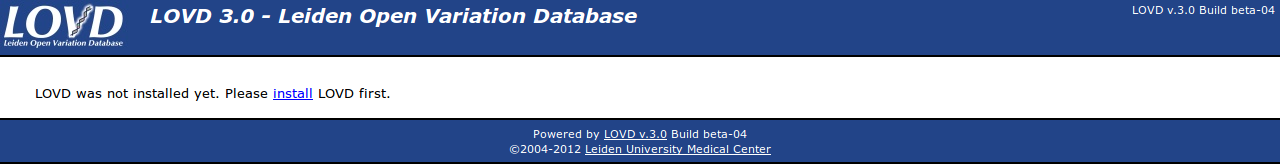
\includegraphics[width=\linewidth]{c02s02_screenshot_not_installed.png}}%
  \caption{%
    When pointing your browser to the LOVD location, it will tell you it's not installed yet.
    Click the link to start the install process.}
  \end{shaded}
\end{figure}

LOVD will first check a few requirements.
Both the PHP and MySQL versions will be checked, to make sure your LOVD will function properly on your webserver environment.
Also some settings of the web server, PHP and MySQL will be checked.
Finally, LOVD will check if your config file has been hidden.
If all looks well, LOVD will tell you all requirements are OK and you're ready to start installing LOVD.
\vskip \baselineskip

Installing LOVD consists of only 4 simple steps and will take only a couple of minutes, or less.

\begin{figure}[ht]
  \begin{shaded}
  \frame{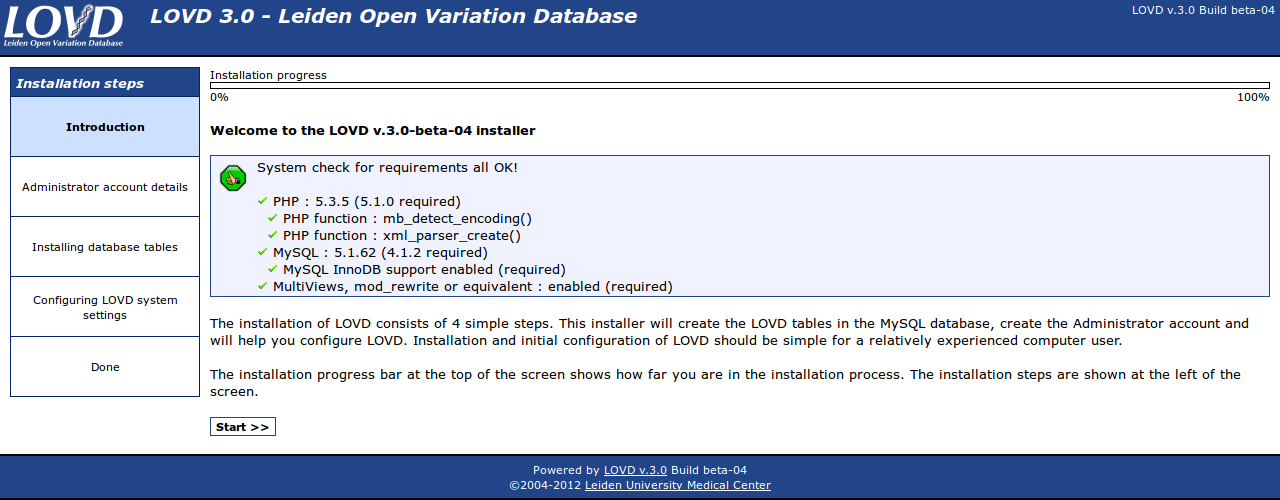
\includegraphics[width=\linewidth]{c02s02_screenshot_installer_01.png}}%
  \caption{If all requirements are OK, you're ready to start installing LOVD.}
  \end{shaded}
\end{figure}



\subsection{Administrator account details}
Fill in the database administrator data to install LOVD.
The database administrator will be the first user registered with LOVD and has full access to all of LOVD's functionalities.
The database administrator is the only user capable of creating manager accounts.
Managers can only create curator and submitter accounts.

\begin{figure}[ht]
  \begin{shaded}
  \frame{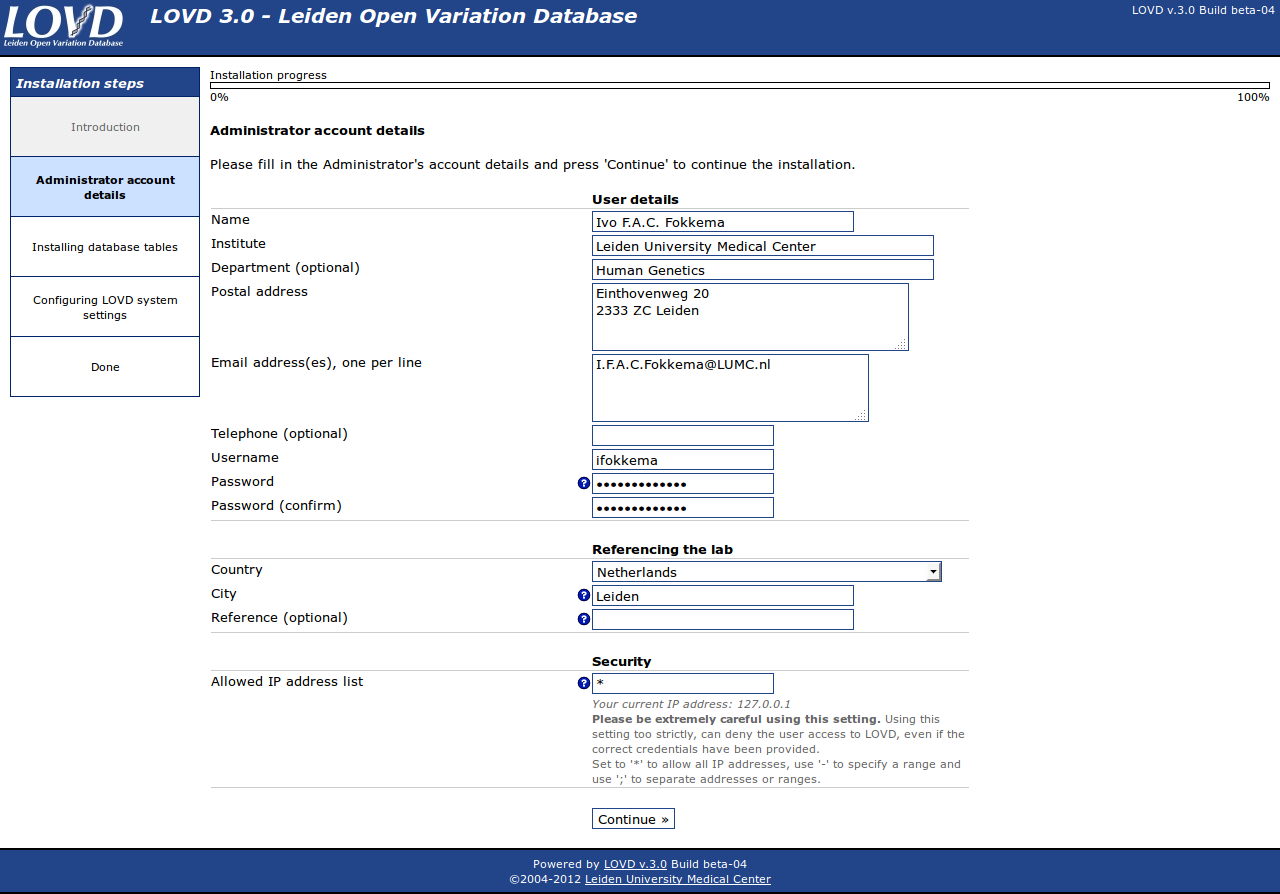
\includegraphics[width=\linewidth]{c02s02_screenshot_installer_02.png}}%
  \caption{The database administrator registration form, with example data filled in.}
  \end{shaded}
\end{figure}

Most of the form is pretty straight forward, but I will highlight one field - ``Allowed IP address list''.
An IP address is an address a computer is known by on the network.
To help prevent others to try and guess the username/password combination,
you can restrict access to the database administrator account to a number of IP addresses or ranges.
This also means you need to be very careful with this setting, as being too restrictive may lock you out of your account.
The default, unrestricted, value is *.

\begin{infotable}
The database administrator is the absolute owner of the LOVD installation.
Not only is he the only one that can uninstall LOVD from the database using the uninstaller,
he will also be able to create, edit or delete all user accounts in the system and
(depending on the settings) receive submission and registration notifications.
\end{infotable}

After completing the database administrator account details, click the ``Continue \guillemotright'' button at the bottom.
LOVD will apply a simple username and password quality check.
If LOVD tells you that the provided details are OK, click the ``Next \guillemotright'' button.



\subsection{Installing database tables}
The next step is to create and fill all necessary LOVD database tables.
LOVD will do this automatically, and you can watch the progress bar complete while the tables are created,
the country list filled, the database administrator account created, the custom columns preconfigured,
the standard columns enabled, and the custom links generated.
This may take a while on non-optimal conditions, so please be patient.
When everything is done, a ``Next \guillemotright'' button appears - click it to continue.

\begin{figure}[ht]
  \begin{shaded}
  \frame{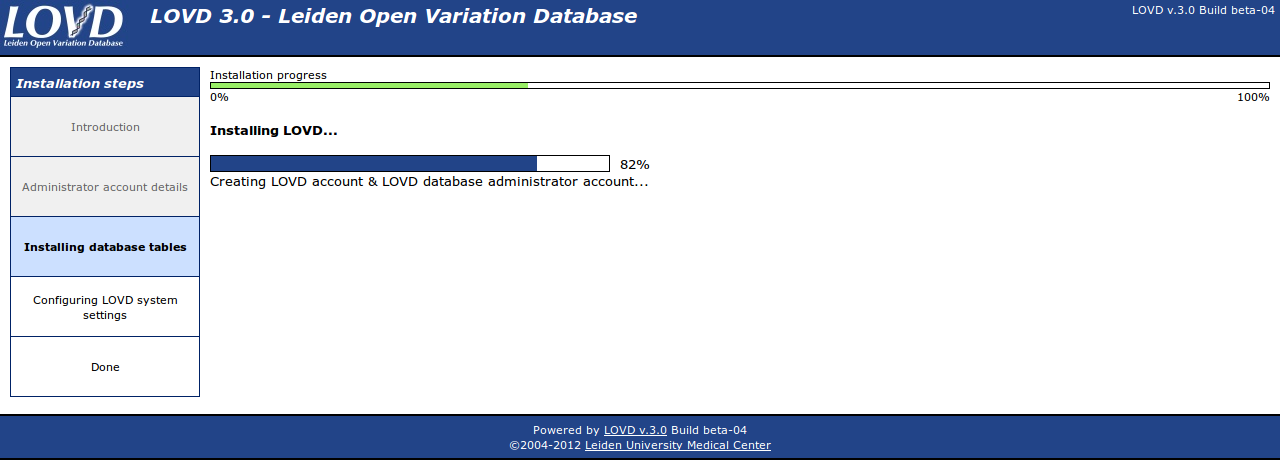
\includegraphics[width=\linewidth]{c02s02_screenshot_installer_03.png}}%
  \caption{Watch the progress bar complete while LOVD informs you which part of the database table installation is currently in progress.}
  \end{shaded}
\end{figure}



\subsection{Configuring LOVD system settings}
The final form in the installation process is completing the initial configuration of the LOVD system settings.
These settings can be changed after installation at any time through the LOVD setup.

The only setting that cannot be changed at a later time, is the install lock, which is checked by default.
Setting the uninstall lock will prevent uninstallation of LOVD by the database administrator.
The only way to remove this lock is directly through the MySQL database backend.

\begin{figure}[ht]
  \begin{shaded}
  \frame{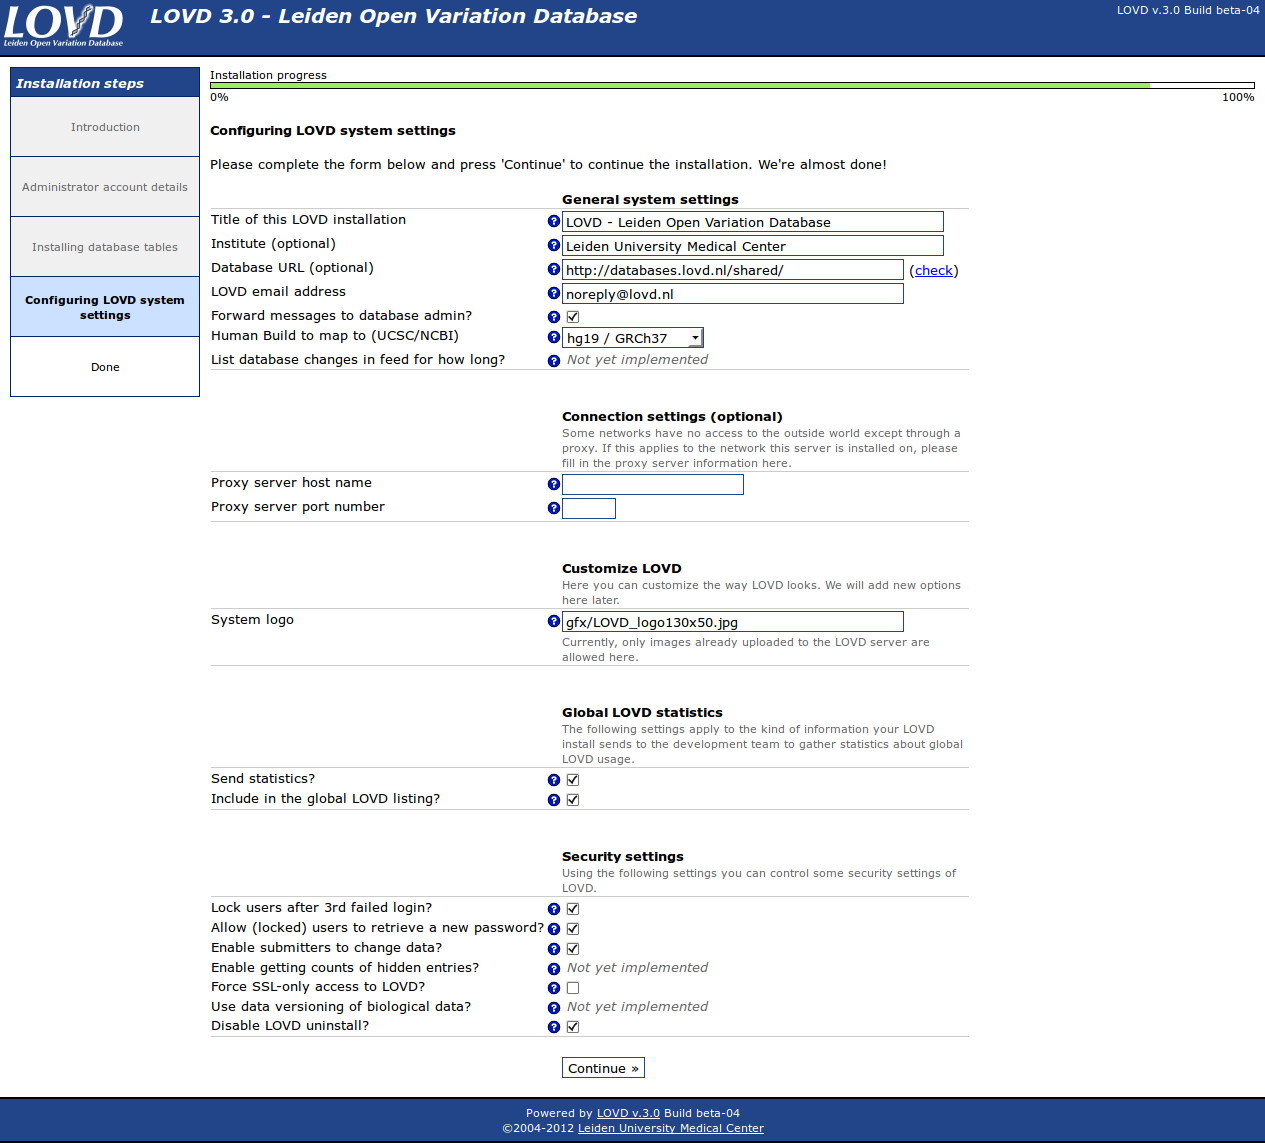
\includegraphics[width=\linewidth]{c02s02_screenshot_installer_04.png}}%
  \caption{The system settings form, with example data filled in.}
  \end{shaded}
\end{figure}

For more information on the options of the LOVD system settings, see the \hyperlink{sec:system_settings}{LOVD system settings} section of the manual.
\vskip \baselineskip

After filling in the form, click ``Continue \guillemotright''.
If everything was filled in correctly, LOVD will register the LOVD system settings.
Click ``Next \guillemotright'' to continue to the last step.
Almost done!



\pagebreak[4] % Break the page here (up to 4; 4 is very persistent)
\subsection{Done}
% FIXME; to be honest nothing is done in this step... so... kill it?
When everything has been filled in and stored correctly, the installation is complete.
Now that you're done installing LOVD, click the ``Continue to Setup area \guillemotright'' button to be forwarded to the \hyperlink{chap:setup}{LOVD setup area}.
From there, you can perform the most important actions for managers in LOVD,
 such as creating new gene databases or disease information entries,
 registering new user accounts or authorizing curators, or manage the custom columns and links.
The button to create a new gene will be highlighted, as a suggestion of your next step!
\clearpage % Makes the hyper target actually point to the right place.










\hypertarget{chap:setup}{}
\chapter{LOVD Setup}

To change system-wide settings, but also to perform actions with system-wide effects, start at the LOVD setup area.
The setup area is only available for managers and the database administrator and can be accessed by clicking on the ``Setup'' tab in the menu.
If you do not see a ``Setup'' tab, you first need to log into the system with a manager or administrator account.
\vskip \baselineskip

The LOVD setup shows some statistics on the left of the screen, like date of installation, number of registered users and variant counts, separated by status.
Furthermore, there are two columns of options.
The left column has options for the system settings, authorized users, the custom columns, custom links, full data download and the LOVD system logs.
The right column has options for genes, transcripts, diseases, individuals and variants.
Some of the general options from the LOVD setup are also available through the Setup tab's dropdown menu,
 allowing you to quickly navigate to other setup options without having to go through the setup main page.
The other options shown in the setup area are available through their own tab's dropdown menus.
\vskip \baselineskip

In this chapter, we will describe changing the LOVD system settings, how to check, search and clean up the LOVD system logs, and how to uninstall LOVD.
The other actions available from the LOVD setup are described in their respective chapters (\hyperlink{toc}{see the table of contents}).





% FIXME: I've been trying multiple things to prevent these lists from breaking over one page.
% The most successful was an attempt in creating a new command "\mynobreakpar" that supposedly creates a par that doesn't break.
% The effect was that the text was more compressed (ugly!!!) to try and prevent a broken item, but it still breaks and anyway I just want it to leave space at the bottom of the page instead of compressing everything.
% Writing \nopagebreak in every freaking line is too much, so I checked out "needspace": http://texblog.net/latex-archive/layout/prevent-page-breaks/
% However, \needspace just dumps space there, so if it's not breaking there because of a change of text in front of it, it now shows a big empty part. Ugly, too.
% Now settled for \pagebreak[] commands.
\hypertarget{sec:system_settings}{}
\section{LOVD system settings}
\begin{wrapfigure}[3]{r}{8cm} % Only wrap for 3 lines
  \vspace{-25pt}
  \begin{leftbar}
    Required level: Manager\\
    Available from: LOVD 3.0 Build 01
  \end{leftbar}
\end{wrapfigure}
The LOVD system settings allow you to adapt your LOVD installation to your preferences.
For instance by changing the installation's displayed name or email address (general settings),
 proxy server settings (connection settings), settings on statistics, or the security settings.

To view or edit the LOVD system settings, click on the ``Setup'' tab, then on ``View and change LOVD System settings (...)'',
or move your mouse over the ``Setup'' tab and click the ``LOVD system settings'' menu option from the dropdown list.



\subsection{General system settings}
\begin{description}
  \item[Title of this LOVD installation] \hfill \\
  This title will be shown on the top of every page, above the menu tabs.
  The default value is ``LOVD - Leiden Open Variation Database''.
  \item[Institute] \hfill \\
  The institute which runs this database is displayed in the public area and in emails sent by LOVD.
  It's commonly set to a laboratory name or a website name.
  If it's not specified, LOVD will use the (autodetected) website name LOVD has been installed on.
  \pagebreak[4] % Break the page here (up to 4; 4 is very persistent)
  \item[Database URL] \hfill \\
  This is the URL with which the database can be accessed by the outside world, including ``http://'' or ``https://'',
   and is not necessarily the URL you are using right now to access the database.
  It will also be used in emails sent by LOVD.
  This field is mandatory if you select the ``Include in the global LOVD listing'' option.
  \\
  If you click the ``check'' link, LOVD will verify or try to predict the value.
  \item[LOVD email address] \hfill \\
  This email address will be used to send emails from LOVD to users.
  LOVD needs this address to prevent problems with spam filters, to make sure that emails from LOVD arrive.
  Please note that although strictly speaking this email address does not need to exist,
   we recommend that you use a valid address to make sure that bounces of emails sent from LOVD
   (to submitters or curators) are still caught by someone, so that they can be handled.
  \item[Forward messages to database admin] \hfill \\
  With this setting enabled, LOVD will forward messages to the database administrator about submitter registrations, submissions, and such.
  \item[Human Build to map to (UCSC/NCBI)] \hfill \\
  This value can only be set during installation, and cannot be changed later.
  It defines on which version of the Human Build (hg18/Build 36.1 or hg19/GRCh37) genomic variants are described.
  Links to the UCSC and Ensembl genome browsers and the NCBI sequence viewer also depend on this setting.
  \\
  From LOVD 3.0-beta-07, the hg18 setting is no longer available for new LOVD installations, although it will remain to be supported.
  When hg20 will come out, LOVD will start supporting multiple genome builds per installation.
  \item[List database changes in feed for how long?] \hfill \\
  \emph{Note: Not yet implemented!}
  \\
  LOVD includes a ``newsfeed'' that allows users to get a list of changes recently made in the database.
  Select here how many months back you want changes to appear on this list.
  Set to ``Not available'' to disable the newsfeed.
\end{description}



\subsection{Connection settings (optional)}
Some networks have no access to the outside world except through a so-called proxy server
 (\href{http://en.wikipedia.org/wiki/Proxy_server#Forward_proxies}{more info on WikiPedia}).
If this applies to the network this server is installed on, please fill in the proxy server information here.
\begin{description}
  \item[Proxy server host name] \hfill \\
  The host name of the proxy server, such as ``www-cache.institution.edu''.
  \item[Proxy server port number] \hfill \\
  The port number of the proxy server, such as 3128.
  \item[Proxy server username] \hfill \\
  In case the proxy server requires authentication, please enter the required username here.
  \item[Proxy server password] \hfill \\
  In case the proxy server requires authentication, please enter the required password here.
\end{description}



\pagebreak[4] % Break the page here (up to 4; 4 is very persistent)
\subsection{Customize LOVD}
Here you can customize the way LOVD looks.
Right now, there is only one option included, we will add more later.
\begin{description}
  \item[System logo] \hfill \\
  If you wish to have your custom logo on the top left of every page instead of the default LOVD logo,
   enter the path to the image here, relative to the LOVD installation path.
  If left empty, it will be set to the default value, which is ``gfx/LOVD\_logo130x50.jpg''.
  Currently, only images already uploaded to the LOVD server are allowed here.
\end{description}



\pagebreak[0] % ``Please'' break the page here (up to 4; 4 is very persistent)
\subsection{Global LOVD statistics}
Your LOVD installation can send some general information on your installation back to us.
We use this information to see how many LOVDs there are worldwide, which versions of LOVD are currently in use,
 how LOVD is being used (amount of data), to see what type of software is used to run LOVD and to construct the public list of LOVD installs.
\begin{description}
  \item[Send statistics] \hfill \\
  When this setting is enabled, LOVD will collect general usage statistics and send this to us.
  The following information is sent: the number of submitters, genes, individuals, variants and unique variants in your system.
  No specific information is sent, just the numbers.
  \hypertarget{item:include_in_listing}{}
  \item[Include in the global LOVD listing] \hfill \\ %% FIXME; When LOVD 3.0 site has such a list, use that URL here.
  On our website, we keep a \href{http://www.lovd.nl/2.0/index_list.php}{list of public LOVD installations}.
  This list is also feeding our \href{http://www.lovd.nl/LSDBs}{worldwide LSDB list},
   through which submitters can locate databases for a specific gene to submit data to.
  If you enable the ``Include in the global LOVD listing'' setting, your LOVD installation will send us all the information we need to build these lists:
   the LOVD installation's name, the URL, the available gene databases, the date of last update of the gene databases,
   the disease abbreviations and names of the diseases related to these genes and finally the names,
   institutes and email addresses of the curators of these gene databases.
  If you change this setting, please allow one day for the setting to take effect.
\end{description}



\hypertarget{ssec:security_settings}{}
\subsection{Security settings}
In this section you can control some security settings of LOVD.
\begin{description}
  \item[Lock users after 3rd failed login?] \hfill \\
  With this setting enabled, submitters, curators and managers will be locked out of the system after they have provided the wrong password three times.
  A manager or, in the case of a locked manager, the database administrator needs to unlock the user's account once it's locked.
  \\
  This does \emph{not} affect the database administrator account.
  \item[Allow (locked) users to retrieve a new password?] \hfill \\
  If a submitter, curator, or manager has lost his password, enabling this ``I forgot my password''
   feature allows them to receive a unlocking code in their email with which they can unlock their account and choose a new password.
  \item[Enable submitters to change data?] \hfill \\
  This setting allows submitters to make changes to data previously submitted by them or assigned to them.
  % FIXME: implement!
  % Changes made by submitters will be reported to the curators by email.
  \item[Enable getting counts of hidden entries?] \hfill \par
  \emph{Note: Not yet implemented!}
  \\
  Enabling this feature allows the public to find the number of entries in the database
   (including hidden entries) matching one or more search terms on a specified set of columns.
  This feature will only mention the number of variant entries matched, without showing them.
  % FIXME: Implement!
  % The columns which can be used for this type of searching, can be configured ....
  \item[Force SSL-only access to LOVD?] \hfill \\
  SSL is a secure protocol allowing for encryption of data sent between you and LOVD.
  When you record sensitive individual information in LOVD, you \emph{\textbf{should}} enable this setting,
   as the individual information can otherwise be ``sniffed'' off the network.
  If you do not record sensitive information, enabling SSL is \emph{recommended}.
  \item[Use data versioning of biological data?] \hfill \\
  \emph{Note: Not yet implemented!}
  \\
  Versioning allows you to see all previous versions of a certain data entry (individuals, variants,
   phenotype information, etc) and allows you to return the entry to a previous state.
  Please note that this feature requires quite a lot of space in the database.
  Disabling this feature later will not free any space, just prevent more space from being used.
\end{description}





\section{System logs}
\begin{wrapfigure}[3]{r}{8cm} % Only wrap for 3 lines
  \vspace{-25pt}
  \begin{leftbar}
    Required level: Manager\\
    Available from: LOVD 3.0 Build 01
  \end{leftbar}
\end{wrapfigure}
System logs were introduced in LOVD 2.0 to allow authorized users to keep track of events in LOVD.
This can be for security purposes, to follow each other's progress when working together,
or to track down errors in case something went wrong.
The logs are initiated when LOVD is installed.



\subsection{What is logged by LOVD}
LOVD logs four types of events: authorization events and errors, general events, general errors, and installation and upgrade events.
In case the event or error was triggered by an authorized user, the username of this user is also logged.

\subsubsection{Authorization events and errors (``Auth'')}
This list stores all successful and unsuccessful login attempts and password reset attempts.
In all cases, the IP address from where the login or password reset attempts have been made, is also logged.
For successful and unsuccessful login attempts the given username and the length of the given password is stored,
 so you can easily uncover brute force attempts where in general the attacker will try many random passwords.
If a user can't log in because of the IP restriction on the account, the current IP restriction is also stored in the log entry.
Please note that it is recommended to have LOVD lock user accounts after three failed login attempts.
See subsection \hyperlink{ssec:security_settings}{Security settings} for more information.

% TODO: Insert list of possible log options, or at least a link to an appendix where they are mentioned.

\subsubsection{General events (``Event'')}
General events are logged to show a user's activity, to allow collaborating users to track each other's
 activities or to check what happened to a certain data entry over time.

% TODO: Insert list of possible log options, or at least a link to an appendix where they are mentioned.

\subsubsection{General errors (``Error'')}
Whenever an unrecoverable error occurs, LOVD logs the error and stops processing.
Also some non-fatal errors are logged, such as when only part of the requested action could be completed.
In principle, during any database event, an error can occur.
This is then logged under the name of the event, so any of the event names used in the general event log can also be found in the error log.
% TODO: In the below table you can find the event names that appear exclusively in the error log. If you find any other event name in the error log, see the above table.

\subsubsection{Installation and upgrade events (``Install'')}
LOVD creates a log entry on completion of the LOVD installation procedure.
Also, after each upgrade, LOVD will add an entry stating from which version to which version it has been upgraded,
 and how many database queries have been used for the upgrade.
Also errors during an LOVD upgrade, might they occur, will be logged here.



\subsection{Viewing and searching through the logs}
To browse the system logs, click the ``View system logs'' option of the ``Setup'' tab dropdown menu,
 or the ``View, search and delete system logs'' link in the setup area.
The system log overview is fully searchable and sortable, allowing you to find log entries quickly.

The ``Log'' column shows the type of log every - \emph{Auth}, \emph{Event}, \emph{Error} or \emph{Install}.
The ``Date'' column shows the date the log entry was created.
The ``User'' column shows, if available, which user caused the log entry to be created.
The ``Event'' column lists the type of event that occurred.
Finally, the ``Entry'' column provides more information about the event that has occurred.
For login attempts, it will contain the IP address of the user attempting to log in.
For most event types, it will include the ID of the entry that was created, edited or deleted.
%TODO:
% A full list of event names is listed in the Appendix.
%\\
%\par
%TODO
% Information on how to sort and search in the LOVD overviews, please see section ...



\subsection{Removing log entries}
\begin{wrapfigure}[4]{r}{5cm} % Only wrap for 4 lines
  \vspace{-25pt}
  \begin{framed}
    \raisebox{-0.5mm}{
\includegraphics[width=4mm]{cross.png}} Delete log entry\\
    \raisebox{-0.5mm}{
\includegraphics[width=4mm]{options.png}} Options menu button
  \end{framed}
\end{wrapfigure}
To remove a single log entry, click on the red cross in the 6th column.
To remove multiple log entries at once, first apply as many search terms on the log entries as needed to restrict the view to the entries you want to delete.
Either manually select the checkboxes next to the entries you want deleted,
 or click the option button on the top left of the log overview, and select the ``Select all ... entries'' option,
 after which you can deselect log entries you do not want deleted.
Then, open the option menu again and click the ``Delete selected entries'' option.
Please note that deleting log entries can not be undone.





\pagebreak[4] % Break the page here (up to 4; 4 is very persistent)
\section{Uninstalling LOVD}
\begin{wrapfigure}[3]{r}{8cm} % Only wrap for 3 lines
  \vspace{-25pt}
  \begin{leftbar}
    Required level: Database administrator\\
    Available from: LOVD 3.0 Build 01
  \end{leftbar}
\end{wrapfigure}
Only the database administrator can uninstall LOVD, provided the uninstall lock has not been set during installation of LOVD.
The uninstall lock is set within the MySQL database and can only be removed by directly accessing MySQL.
If you know how to handle MySQL, you can also uninstall LOVD through MySQL directly, by removing all LOVD tables, but this is not recommended.
\vskip \baselineskip

To uninstall LOVD and remove all data stored in LOVD, click on the ``Uninstall LOVD'' link in the setup area.
This link is only available if the uninstall lock is disabled.
You will need to fill in the database administrator's password twice to complete the uninstallation process.

\begin{warntable}
Once you have uninstalled LOVD, you have lost all variant and individual information.
If you wish to store these data elsewhere, make sure you download all data first!
\end{warntable}

\begin{infotable}
Please note that the LOVD uninstaller will not remove the LOVD files itself, just the database tables that it has created during install.
Thus, to completely remove LOVD from the system, also remove the files from the server.
\end{infotable}










\chapter{Authorized users}
In LOVD 3.0, \emph{authorized users} are everyone who registered for an account at the LOVD installation,
 including the database administrator who created his account during the installation process.
The authorized users come in five levels; the database administrator of which there is only one, managers, curators, collaborators and submitters.
The different levels of users are described in more detail below.

Registering for an account is necessary to be able to submit data or to become a gene curator.
Directly after registering, you are allowed to submit individual, phenotype and variant data to the database,
 but the data needs to be checked and published by a \emph{curator} or a \emph{manager}.
Curators and managers can submit and publish data in one step.



\hypertarget{ssec:user_levels}{}
\subsection{User levels}
\subsubsection{Database administrator}
The database administrator is the first user within LOVD; this account is created during the installation of LOVD.
After installation, the database administrator can create other users (managers, curators and submitters) in the system, if desired.
These users can also register themselves, after which the database administrator can upgrade them.

The administrator has full access to all areas and settings of LOVD.
The administrator is also the only user who can uninstall LOVD, provided the uninstall lock has not been set during LOVD installation.
\vskip \baselineskip

When the ``Forward messages to database admin'' setting in the \hyperlink{sec:system_settings}{LOVD system settings} is enabled,
 the database administrator will receive copies of submitter registrations and data submissions or edits.

\subsubsection{Manager}
A manager has access to almost everything the database administrator has access to.
However, the manager is not able to create new managers or to edit existing managers.
Also, a manager cannot uninstall LOVD even if the uninstall lock is not in place.
\vskip \baselineskip

A manager can only be created by the administrator and often assists the administrator or takes over the customisation of LOVD for the curators.

\subsubsection{Curator}
The curator level user is actually a submitter, which has been given curatorship of one or more genes.
Therefore, a curator only has access to the gene databases he is appointed to, and not to the system-wide setup area.
However, also the database administrator or a manager can act as a curator by being appointed to certain genes,
 but in this case there is of course no restriction in access.
\vskip \baselineskip

To assign a user to become curator, follow the steps explained in section
 ``\hyperlink{sec:gene_assign_curators}{assigning curators and collaborators}'' (available for managers and up).

\subsubsection{Collaborator}
The collaborator level user is a new type of user, introduced in LOVD 3.0.
Collaborators are submitters with read access to non-public data on a certain given gene.
Just like curators, these users must be appointed to genes by managers or the database administrator.
See section ``\hyperlink{sec:gene_assign_curators}{assigning curators and collaborators}'' for more information.

\subsubsection{Submitter}
Submitters have no special rights except to submit data to the database, which then needs to be checked and published by curators or managers.
Depending on the LOVD system settings, submitters are also able to edit the data they have submitted previously.

Submitter accounts can also be created, edited or deleted by managers or the database administrator, although usually this should not be necessary.
Curators do not require a separate submitter account; they can use their curator account to submit new data.





% FIXME: Create section on how to deal with the user viewlist.

%From the setup area, click the "Manage authorized users" link. This shows a list of the authorized users, sorted by default by the user's level and name.

%The Status column provides a quick view of the user's status:
% The user is locked.
% The user is currently logged in.
% The user is currently logged off.
%Deleted users show at the bottom of the list and are greyed out.

%Editing submitters
%From the setup area, click the "Manage submitters" link. This shows a list of the authorized users, sorted by default by the submitter's country and name.

%The Status column provides a quick view of the submitter's status:
% The submitter is locked.
% The submitter is currently logged in.
% The submitter is currently logged off.
%Deleted submitters show at the bottom of the list and are greyed out.





\hypertarget{sec:submitter_register}{}
\section{Registering a new account}
\begin{wrapfigure}[3]{r}{8cm} % Only wrap for 3 lines
  \vspace{-25pt}
  \begin{leftbar}
    Required level: None (public)\\
    Available from: LOVD 3.0 Build 01
  \end{leftbar}
\end{wrapfigure}
\begin{warntable}
Please note that you do \textbf{NOT} need to register to view the data available in the database.
You only need an account for submitting new variant data.
\end{warntable}
Anyone can create a new submitter account.
For collaborators, curators or managers, registering as a submitter is often the first step;
 their account can then be upgraded by a manager or the database administrator, respectively.
The major difference between registration and direct creation of a new account by a manager or the database administrator,
 is that the registration can be performed by the public, and therefore it requires you to be logged out of LOVD.
The registration form is protected using a \emph{reCAPTCHA} module, which makes sure the form can only be used by humans, and not by spam bots.
\vskip \baselineskip

To register a new submitter account, click the ``Register as submitter'' link on the top right corner of the screen, next to the ``Log in'' link.
First, you are asked to provide an ORCID ID, if you have one.
\href{http://about.orcid.org/}{ORCID} provides a persistent digital identifier that distinguishes you from every other researcher and,
 through integration in key research workflows such as manuscript and grant submission,
 supports automated linkages between you and your professional activities ensuring that your work is recognized.
If you don't have an ORCID ID yet, you can get one created by using the \href{https://orcid.org/register}{register} link also given on the page.
If you don't want to register at ORCID at this time, click the ``I don't have an ORCID ID \guillemotright'' button to continue to the registration page.
If you do have an ORCID ID, fill it in and click the ``Continue \guillemotright'' button.
Your ORCID ID will be verified, and the associated data is shown on the screen.
If this data is correct, click ``Yes, this is correct \guillemotright'' to continue to the registration page.
As much information as possibly will be pre-filled for you.
If the information shown is not correct, click ``\guillemotleft{} No, this is not correct''
 so you can try and enter a correct ORCID ID or register without using one.



\pagebreak[4] % Break the page here (up to 4; 4 is very persistent)
\subsection{User details}
This part of the registration form contains the basic fields with which the user identifies himself.
\begin{description}
  \item[Name] \hfill \\
  Please enter your name in the way you want to be referenced to; usually in the format ``<First name> <Last name>''.
  \item[Institute] \hfill \\
  The institute for which you work.
  \item[Deparment] \hfill \\
  If your institute consists of department, please enter the department for which you work.
  \item[Postal address] \hfill \\
  Please provide the full postal address of your institute.
  \item[Email address(es), one per line] \hfill \\
  Your account can hold multiple email addresses, which will all receive notifications sent by LOVD.
  This is useful if you're sharing an account with a colleague, or when you would like to also get emails on a different account.
  You can enter as many email addresses as you like, one email address per line, no spaces, quotes or other special characters allowed.
  \item[Telephone] \hfill \\
  Optionally, provide your phone number where you can be reached.
  \item[Username] \hfill \\
  LOVD requires the username to be 4 to 20 characters long, and starting with a letter followed by letters, numbers, dots, underscores and dashes only.
  \item[Password] \hfill \\
  LOVD requires the password to be at least 4 characters long, containing at least one number or special character.
  Please choose your password wisely; don't use the same password as your username and better not use words that are in a dictionary.
  \item[Password (confirm)] \hfill \\
  To make sure you din't make a typo while entering your password, please repeat it so we can check if the two fields are equal.
\end{description}



\subsection{Referencing the lab}
This part describes the reference that LOVD makes to your institute.
\begin{description}
  \item[Country] \hfill \\
  Please select the country from the given list.
  \item[City] \hfill \\
  Even though you entered the city also in the address field above, please enter it here as well.
  It's used for sorting purposes when creating a list of the institutes registered to the installation.
  \item[Reference] \hfill \\
  Your submissions will contain a reference to you in the format "Country:City" by default.
  You may change this to your preferred reference here.
\end{description}



\subsection{Security}
To prevent unauthorized use of your account, we implemented a security feature that you can configure here.
\begin{description}
  \item[Allowed IP address list] \hfill \\
  \emph{
    Note: Please be extremely careful using this setting.
    Using this setting too strictly, can deny you access to LOVD, even if the correct credentials have been provided.
  }
  \\
  An IP address is an address a computer is known by on the network.
  To help prevent others to try and guess your username/password combination, you can restrict access to your account to a number of IP addresses or ranges.
  For instance, to make sure your account can only be used when accessed from your institute or from your home.
  \\
  Set to ``*'' to allow all IP addresses, use ``-'' to specify a range (like ``192.168.0.1-20'') and use ``;''
   to separate addresses or ranges (like ``192.168.0.1;192.168.1.34'').
\end{description}



\subsection{Registration authentication}
To prevent automatic submission of the registration form, we implemented a \href{http://www.google.com/recaptcha}{reCAPTCHA} module.
In the provided text field, type the two words you see in the image.
This will proof that you are a human and not a computer.
\vskip \baselineskip

After completing the form, press the ``Register'' button.
LOVD sends you a confirmation of your registered information through email.
If the ``Forward messages to database admin'' setting in the \hyperlink{sec:system_settings}{LOVD system settings} is enabled,
 the database administrator also receives a copy of your data.





\section{Creating new user accounts}
\begin{wrapfigure}[3]{r}{8cm} % Only wrap for 3 lines
  \vspace{-25pt}
  \begin{leftbar}
    Required level: Manager\\
    Available from: LOVD 3.0 Build 01
  \end{leftbar}
\end{wrapfigure}
Besides the public registration form, managers can also create new users.
This offers the advantage that the new user's level can be set to the required level in the same step, and the manager does not need to log out first.
You can create a new user by clicking on the ``Create a new user account'' option from the ``Users'' tab dropdown menu,
 or the ``Create a new authorized user or submitter'' link in the setup area.
The process is largely equal to the submitter registration process, except that there is no reCAPTCHA test but
 instead you must enter your password for authorization, and the form has some additional fields, explained below.



\subsection{User details}
This section contains one additional field, compared to the registration page.
\begin{description}
  \item[Must change password at next logon] \hfill \\
  If you want to force the user to pick a new password after logging in for the first time, select this checkbox.
  The user will not be able to work with LOVD until he has changed his password.
\end{description}



\pagebreak[4] % Break the page here (up to 4; 4 is very persistent)
\subsection{Security}
This section contains more options when creating a new user account for a new user, compared with when registering your own account.
\begin{description}
  \item[Level] \hfill \\
  Managers only see the option ``Submitter'' here.
  The database administrator may also select ``Manager'' here.
  Please note that to create a Curator account, you need to create a Submitter and then grant this user rights on the necessary genes.
  See section ``\hyperlink{sec:gene_assign_curators}{Assigning curators and collaborators}'' for more information.
  For a complete description on all user levels, see the subsection ``\hyperlink{ssec:user_levels}{User levels}''.
  \item[Locked] \hfill \\
  Users can be locked, which blocks access to LOVD even if they provide the correct username and password.
  This locking happens when too many times an invalid password was given while logging in with this username
   (depending on the \hyperlink{sec:system_settings}{LOVD system settings}), or it can be done manually.
\end{description}



\subsection{Other fields}
This option is only available while creating a new user, it's not shown on the submitter registration form.
\begin{description}
  \item[Send email with account details to user] \hfill \\
  When enabled, the user's details will be emailed to the email address(es) given, informing the user immediately about his account details.
  The submitter registration form does not have this checkbox, but this feature is \emph{always} active for submitter registrations.
\end{description}





\section{Editing user accounts}
\begin{wrapfigure}[3]{r}{8cm} % Only wrap for 3 lines
  \vspace{-25pt}
  \begin{leftbar}
    Required level: Submitter\\
    Available from: LOVD 3.0 Build 01
  \end{leftbar}
\end{wrapfigure}
Every user in LOVD can edit their own account.
Editing other user's accounts requires you to have a level higher than the user you are trying to edit.
Managers can edit submitter accounts (including collaborators and curators).
The database administrator can also edit manager accounts.
\vskip \baselineskip

To edit your own account, click the ``Your account'' link on the top right-hand side of the screen, which leads directly to your account overview.
Then, click the ``Options'' button and click ``Update your registration''.
\\
To edit someone else's account, click the ``Users'' tab.
Locate the user you wish to edit by searching or browsing through the given user listing.
Clicking the entry will direct you to the user's account details.
If you have permission to edit this account, you'll see an ``Options'' button.
Click it and click ``Edit user''.
\vskip \baselineskip

The fields on the form are explained in the section ``\hyperlink{sec:submitter_register}{Registering a new account}''.
Please note that the ``New password'' fields are optional when editing an existing user account.
You only fill them in when you want to change the password.
\\
After you submit the form, LOVD redirects you automatically back to the user's account details.





\section{Locking users out of the system}
\begin{wrapfigure}[3]{r}{8cm} % Only wrap for 3 lines
  \vspace{-25pt}
  \begin{leftbar}
    Required level: Manager\\
    Available from: LOVD 3.0 Build 01
  \end{leftbar}
\end{wrapfigure}
A user is automatically locked if a wrong password is used three times while logging in with this username,
 provided this security setting is enabled (see section ``\hyperlink{sec:system_settings}{LOVD system settings}''),
 but this lock may also be placed onto, or removed from an account manually.
Locking or unlocking a user account requires you to have a level higher than the user you are trying to lock or unlock.
Proceed to the user's account details page through the ``Users'' tab.
Open the ``Options'' menu, and click the ``Lock user'' option.
If the user is already locked, there will be an ``Unlock user'' option.
\\
The ``Lock user'' and ``Unlock user'' menu options are quick ways to deny or allow access to LOVD,
 although it can also be accomplished through the ``Edit user'' option.
\vskip \baselineskip

Users who are logged in, can also be booted out of the system.
If a user is logged in, the option ``Force user log out'' is added to the ``Options'' menu.
This will destroy the user's session, causing the user to log out.
Locking the user essentially also causes the user to be logged out of the system the next time the user performs an action,
 although in that case it's not possible for the user to log back in until the account is unlocked.





%\section{Deleting user accounts}
%\begin{wrapfigure}[3]{r}{8cm} % Only wrap for 3 lines
%  \vspace{-25pt}
%  \begin{leftbar}
%    Required level: Manager\\
%    Available from: LOVD 3.0 Build 01
%  \end{leftbar}
%\end{wrapfigure}
%Deleting a user account in LOVD 3.0 is a permanent action.
%
%
%
%Since the user may have created or edited variants, patients, custom columns, custom links etc, permanently deleting the user from the system may leave some references in the database broken. Therefore, deleting a user only disables the user's account and removes the user as a curator from the genes he or she was a curator for, but does not permanently remove the account. A deleted user can therefore be 'revived' by editing the user and unchecking the 'deleted' checkbox.
%If the user is the only curator for one or more genes, and you delete the user, you inherit the curator rights on these 'orphaned' genes. If you want to prevent this, make sure the gene has at least one other curator.
%
%From the user's detailed view, a link named "Delete user" is available if the user has not already been deleted and you have the correct rights on the user account. After clicking that link, you need to confirm deleting the user with your password. Also, if you will take over any genes, this is reported on this confirmation form.
%
%Since the submitter may have created or edited variants and patients, permanently deleting the submitter from the system may leave some references in the database broken and is therefore only possible with submitters not linked to any patients. Deleting a submitter disables the submitter's account, but leaves the account dormant. A deleted submitter can be 'revived' by editing the submitter and unchecking the 'deleted' checkbox.
%
%From the submitter's detailed view, a link named "Delete submitter" is available if the user has not already been deleted. After clicking that link, you need to confirm deleting the submitter with your password. If the submitter is already deleted and has no associated submissions, the account can be permanently deleted by clicking the "Permanently delete submitter" link.










\chapter{Gene databases}
Although in LOVD 3.0 you can enter data into the database without having genes in your installation, the genes still embody an important part of LOVD.
Configuring genes in LOVD allows you to see the effects of variants on transcript level, and draws submitters with variant data to your installation.

Gene databases can also be created automatically for you, when you are importing VCF or SeattleSeq annotated files in LOVD.
However, this chapter deals with manually creating gene databases.
%TODO
%For more information on how to import VCF or SeattleSeq annotated files, see ...
You can create new genes through the \hyperlink{chap:setup}{LOVD setup area}.
Editing and deleting genes is done through the ``Genes'' tab.
Curators assigned to genes can also edit these after they've been created, but can not delete genes.
Emptying genes (removing all associated variant and patient data) and managing its variants is done through the configuration area.
This chapter describes how to create, edit and delete gene databases in LOVD.





\hypertarget{sec:gene_create}{}
\section{Creating a new gene database}
\begin{wrapfigure}[3]{r}{8cm} % Only wrap for 3 lines
  \vspace{-25pt}
  \begin{leftbar}
    Required level: Manager\\
    Available from: LOVD 3.0 Build 01
  \end{leftbar}
\end{wrapfigure}
Creating a new gene database in LOVD is largely automated.
Click the ``Create a new gene entry'' option of the ``Genes'' tab dropdown menu, or the ``Create a new gene database'' link in the setup area.
Fill in the HGNC ID or the gene symbol of the gene you want to create, and click ``Continue \guillemotright''.
LOVD will check if the gene already exists in this LOVD installation, and if the gene symbol or HGNC ID is correct.
For this, it contacts the \href{http://www.genenames.org/}{HGNC website}.
If the gene symbol you used has been replaced by a new one, or if LOVD can find genes for which the given symbol is an alias,
 LOVD will report back the official symbol(s).

\begin{infotable}
Unfortunately, due to some problems on the side of the NCBI, we are unable to handle variants on the mitochondrial genome at this time.
NCBI does not handle the MT genes by their official names, and doesn't allow for automatic retrieval of reference sequences for the MT genes.
When the NCBI has fixed this problem, we will implement support for MT genes.
\end{infotable}

LOVD will show a progress bar while it contacts several webservices to retrieve gene information,
 reference sequence information and available transcript information.
Usually retrieving this information takes about 1-3 seconds, but this depends on the internet connection between
the server and the internet and the current load on the webservices which are contacted.
When LOVD has retrieved all the information, you are forwarded to the data entry form where
 you can review the retrieved information and complete this gene's settings.



\pagebreak[4] % Break the page here (up to 4; 4 is very persistent)
\subsection{General information}
This part describes the bare essentials of the gene information.
Therefore, most of the information in this section has been filled in for you, and some values are fixed to ensure the data is correct.
\begin{description}
  \item[Full gene name] \hfill \\
  This information has been filled in for you, and can't be changed.
  \item[Official gene symbol] \hfill \\
  This information has been filled in for you, and can't be changed.
  \item[Chromosome] \hfill \\
  This information has been filled in for you, and can't be changed.
  \item[Chromosomal band] \hfill \\
  The chromosomal band on which the gene lies, is retrieved from the HGNC.
  You may modify it, if you wish.
  \item[Imprinting] \hfill \\
  If known, please fill in if this gene is imprinted (maternal or paternal) or not.
  \item[Date of creation] \hfill \\
  \emph{Note: This field can only be filled in when creating a gene database and can never be edited afterwards!}
  \\
  The database's date of creation is mentioned on the \hyperlink{sec:gene_homepage}{gene homepage}.
  Today's date will automatically be stored if you leave this field empty, but in case you already
   had a gene database but you're moving it to this LOVD installation, you may want to fill in a different date.
\end{description}



\hypertarget{ssec:relation_to_disease}{}
\subsection{Relation to diseases}
\label{ssec:relation_to_disease}
\begin{description}
  \item[This gene has been linked to these diseases] \hfill \\
  By linking the gene to disease(s), LOVD can help predicting next steps in data submission,
   and the link to the disease information will be shown on the gene homepage.
  If a disease you need is not present in this list, you can click the
   ``configure more diseases'' link below the selection list to create a new disease now.
  Afterwards, reload the gene form so you can select the new disease.
  \\
  Alternatively, create the disease after the gene has been created.
\end{description}



\subsection{Reference sequences}
Collecting variants requires a proper reference sequence.
Without a genomic and a transcript reference sequence the variants in this LOVD database cannot be interpreted properly or mapped to the genome.
When properly configured, LOVD will add links to the Ensembl, NCBI and UCSC genome browsers from the gene homepage, generating a nice visual overview of the variants in the database.
\begin{description}
  \item[Genomic reference sequence] \hfill \\
  Select the genomic reference sequence (NG, NC or LRG accession number).
  Only the references that are available to LOVD are shown.
  Whether there is an LRG available, is determined by contacting the EBI.
  Checking for an available NG reference sequence is done at the NCBI.
  The NC reference sequence is always available, and depends on the chromosome on which the gene lies.
  \item[Transcript reference sequence(s)] \hfill \\
  LOVD retrieves a list of available transcripts from Mutalyzer.
  Mutalyzer currently only supports NCBI reference sequences.
  Please select which transcript you want to use to name the variants in this gene.
  If there are more transcripts, usually you would pick the transcript that encodes for the longest protein,
   or the transcript that is expressed in the tissue you focus your research on.
  If you want to add more transcripts later, or change which transcript(s) you want to use
   for this gene database, see the chapter \hyperlink{chap:transcripts}{Gene transcripts}.
\end{description}



\subsection{Links to information sources}
Here you can add links to other resources that will be displayed on the gene's LOVD gene homepage,
 such as Entrez Gene, OMIM, HGMD or GeneTests, but you can also add links to any website you want.
\begin{description}
  \item[Homepage URL] \hfill \\
  If you have a separate homepage about this gene, you can specify the URL here.
  For the format: use the complete URL, including ``http://'' or ``https://''.
  \item[External links] \hfill \\
  Here you can provide links to other resources on the internet that you would like to link to,
   such as other gene variant databases, or websites with more information about diagnostics.
  If you want to include more than one link, put every link on a new line in this field.
  If you do not want to include a title for this link, simply paste the full URL in this field, such as ``http://DMD.LOVD.nl/''.
  If you do want to include a title, use the format ``Description <URL>'', such as ``Other LOVDs on this gene <http://DMD.LOVD.nl/>''.
  \item[HGNC ID] \hfill \\
  This information has been filled in for you, and can't be changed.
  \item[Entrez Gene (Locuslink) ID] \hfill \\
  This information has been filled in for you, and can't be changed.
  \item[OMIM Gene ID] \hfill \\
  This information has been filled in for you, and can't be changed.
  \item[Provide link to HGMD] \hfill \\
  If you wish to include a link from the gene homepage to the gene's page on the HGMD site, enable this checkbox.
  \item[Provide link to GeneCards] \hfill \\
  If you wish to include a link from the gene homepage to the gene's page on the GeneCards site, enable this checkbox.
  \item[Provide link to GeneTests] \hfill \\
  If you wish to include a link from the gene homepage to the gene's page on the GeneTests site, enable this checkbox.
  \item[This gene has a human-readable reference sequence] \hfill \\
  Although GenBank files are the official reference sequence, they are not very readable for humans.
  If you have a human-readable format of your reference sequence online, please select the type here; ``Coding DNA'' or ``Genomic''.
  \pagebreak[4] % Break the page here (up to 4; 4 is very persistent)
  \item[Human-readable reference sequence location] \hfill \\
% TODO: add link to refseq parser section in manual.
  To create a human-readable reference sequence file, you can use our Reference Sequence Parser.
  It retrieves the reference sequence from Mutalyzer, and formats it into a human-readable
   format with good annotation of the upstream sequence, the exons, the introns, the downstream sequence,
   the predicted protein sequence and the alternative stop codons.
  Fill in the complete URL of the file, including ``http://'' or ``https://''.
\end{description}



\subsection{Customizations}
LOVD allows you to customize the gene homepage by adding citation references, headers, footers, notes and a disclaimer.
The header and footer will also be shown on the variant listings.
\begin{description}
  \item[Citation reference(s)] \hfill \\
% TODO: add link to custom links when in manual.
  Using our PubMed custom link, you can add links to PubMed articles to cite your database or that you want to point visitors to.
  % For more information on how to use custom links, see.....
  \item[Include disclaimer] \hfill \\
  If you want a disclaimer added to the gene's LOVD gene homepage, select your preferred option here.
  \item[Text for own disclaimer] (HTML enabled)\hfill \\
  Only in case you selected the ``Use own disclaimer'' in the field above, you can enter the text here.
  Text in this field will be ignored if you disabled the disclaimer or selected the standard LOVD disclaimer.
  \item[Page header] (HTML enabled) \hfill \\
  If you want a gene-specific header on all public gene-specific pages, please enter the text here.
  \item[Header aligned to] \hfill \\
  In case you defined a page header, here you can select how you want it aligned - left, center or right.
  \item[Page footer] (HTML enabled) \hfill \\
  If you want a gene-specific footer on all public gene-specific pages, please enter the text here.
  \item[Footer aligned to] \hfill \\
  In case you defined a page footer, here you can select how you want it aligned - left, center or right.
  \item[Notes for the LOVD gene homepage] (HTML enabled) \hfill \\
  Text entered here will appear in the General Information box on the gene's homepage.
  In general, curators put additional information about the database here,
   such as how the data in the database was collected, grants supporting this work, or news.
  \item[Notes for the variant listings] (HTML enabled) \hfill \\
  Text entered here will appear below the gene's variant listings.
\end{description}



\pagebreak[4] % Break the page here (up to 4; 4 is very persistent)
\subsection{Security settings}
Using the following settings you can control some security settings of LOVD.
\begin{description}
  \item[Allow public to download variant entries] \hfill \\
  This controls whether or not the public can also make downloads of your gene's variants.
  \item[Allow my public variant and individual data to be indexed by WikiProfessional] \hfill \\
  \emph{Note: Not yet implemented!}
  \\
  If you'll allow the \href{http://www.wikiprofessional.org/}{WikiProfessional} concept web to index your variant and individual data, enable this checkbox.
\end{description}





\hypertarget{sec:gene_homepage}{}
\section{The gene homepage}
\begin{wrapfigure}[3]{r}{8cm} % Only wrap for 3 lines
  \vspace{-25pt}
  \begin{leftbar}
    Required level: None (public)\\
    Available from: LOVD 3.0 Build 01
  \end{leftbar}
\end{wrapfigure}
LOVD automatically generates a gene homepage for every gene created within LOVD.
The gene homepage is the entry point for visitors of a locus-specific database.
In installations where LOVD is used for next-generation sequencing, the gene homepage serves more as a summary page of the gene-specific data in LOVD.
Besides showing the basic information known about the gene in question (symbol, name,
 chromosome band, variant statistics, etc), curators also have quite a few options to customize the gene's homepage.
\vskip \baselineskip

If the gene you wish to view is already selected (its name is on the top of the page), simply click the ``Genes'' tab to open the gene's homepage.
Otherwise, move your mouse over the ``Genes'' tab, and select the ``View all genes'' menu option.
Then, locate the gene you wish to edit by searching or browsing through the given genes listing.
Clicking the entry will direct you to the gene's homepage.

Once on the gene's homepage, the gene will be selected (its name will appear on the very top of the page),
 which allows faster navigation to information related to the gene of interest.
For instance, when a gene is selected and you click the ``Variants'' tab, you are directed to the gene-specific variant overview.
If no gene is selected, clicking on the same tab shows all genomic variants in the database.
If you do not like this behavior, simply move your mouse over a tab, and select a different option from the dropdown menu.
% TODO: STUB!
% Add info about certain fields? Add info about the graphs? Add info about the transcripts shown? Add info about the menu? Maybe in a different subsection?
%LOVD2 wrote (some parts already removed):
%This homepage shows general information on the gene, including links to a list of all PubMed references in the database and a RSS feed subscription link for updates of the gene, combined with links to graphical displays and utilities, the sequence variant tables, links to search forms and links to other external resources.
%\\
%\par
%The "Graphical displays and utilities" table provides links to summary tables, to the Reading Frame Checker, and to external/genome browsers (UCSC, NCBI).
%The summary tables show statistics on all sequence variants in the database, including graphs on the distribution of variants over the gene and the different variant types.
%The Reading Frame Checker generates a prediction of the effect of whole-exon changes.
%The UCSC Genome browser will show the variants in this database as a custom track, so you will have an overview of the variants in relation to their position in the gene.
%The normal view will show the variants labeled with the DNA change, the compact view without these labels.
%The NCBI Sequence Viewer will show a distribution histogram of variants from this database.
%This feature is only available if the gene's transcript reference sequence ID has been filled in in the gene database settings.
%
%Optionally, a download link is also added to the table, with which you can download all of the variant and patient information in the database.
%The unique sequence variants listing shows all unique sequence variants in the database, but no patient data.
%The complete sequence variant listing will show all variants in the database in combination with the patient data associated with them.
%The listing of variants with no known pathogenicity shows all variants that do not appear to have any pathogenic effect on the patient.
%
%The variant listing based on patient origin only works if origin fields have been enabled.
%If enabled, you can create an overview of all variants and patients from a certain geographical or ethnic origin.
%More information on this overview can be found in the Viewing and searching variant and patient data section.
%And finally, if enabled, an option is presented to search through all (including hidden) data to return the number of entries matching your search terms.
%This overview allows you for instance to quickly check if a certain variant is already included in the database (even if it's not yet public) or the amount of entries associated with a certain reference.
%
%The "Links to other resources" table can contain any number of links to external sources, as configured by the gene's curator(s).
%Examples of external sources that LOVD can link to easily are Entrez Gene, OMIM, UniProtKB, HGMD, GeneCards and GeneTests.





\section{Editing a gene database}
\begin{wrapfigure}[3]{r}{8cm} % Only wrap for 3 lines
  \vspace{-25pt}
  \begin{leftbar}
    Required level: Curator\\
    Available from: LOVD 3.0 Build 01
  \end{leftbar}
\end{wrapfigure}
Curators, appointed to a gene database, have the rights to edit its settings.
Managers and up can edit all gene databases in the LOVD installation.
To edit the gene's settings, first proceed to the \hyperlink{sec:gene_homepage}{gene's homepage}.

\begin{wrapfigure}[4]{r}{5cm} % Only wrap for 4 lines
  \vspace{-25pt}
  \begin{framed}
    \raisebox{-0.5mm}{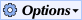
\includegraphics[width=2.1cm]{options_button.png}}\\Options menu button
  \end{framed}
\end{wrapfigure}
Click on the ``Options'' menu button to open up the gene entry's menu.
If you do not see the ``Options'' menu button, you are not logged in or you do not have rights to edit this gene's settings.
In the opened menu, click ``Edit gene information'' to open up the gene's edit form.
The fields on the form are explained in the section ``\hyperlink{sec:gene_create}{Creating a new gene database}''.
After you submit the form, LOVD redirects you automatically back to the gene's homepage.





\hypertarget{sec:gene_delete}{}
\section{Deleting a gene database}
\begin{wrapfigure}[3]{r}{8cm} % Only wrap for 3 lines
  \vspace{-25pt}
  \begin{leftbar}
    Required level: Manager\\
    Available from: LOVD 3.0 Build 01
  \end{leftbar}
\end{wrapfigure}
Only managers and up can delete gene databases from LOVD.
To delete the gene database in question, first proceed to the \hyperlink{sec:gene_homepage}{gene's homepage}.
Click on the ``Options'' menu button to open up the gene entry's menu, and select the ``Delete gene entry'' option.
To complete the removal, you need to fill in your password and submit the form.

\begin{warntable}
Removing a gene can not be undone, you will need to create the gene database again.
If in any doubt, first make a download of the database so that you can restore your data if needed.
Please note that deleting a gene removes also its transcripts in the database and therefore
 all variant annotation on the gene in question, but it \emph{does not remove the genomic variants from the database}.
To remove these as well, you should first empty the gene database, which deletes all its variants and also deletes
 all other connected data such as individuals and phenotypes, as long as these are not connected to other genes as well.
\end{warntable}





\hypertarget{sec:gene_assign_curators}{}
\section{Assigning curators and collaborators}
\begin{wrapfigure}[3]{r}{8cm} % Only wrap for 3 lines
  \vspace{-25pt}
  \begin{leftbar}
    Required level: Manager\\
    Available from: LOVD 3.0 Build 01
  \end{leftbar}
\end{wrapfigure}
Managers and up can assign curators and collaborators to gene databases, as well as revoke curator or collaborator rights.
Directly after creating a new gene database, you are forwarded to the page that allows you to make these changes,
 but you can access that page at any time by using the ``Add/remove curators/collaborators'' link in the
 ``Options'' menu on the \hyperlink{sec:gene_homepage}{gene's homepage}.

\begin{figure}[ht]
  \begin{shaded}
  \frame{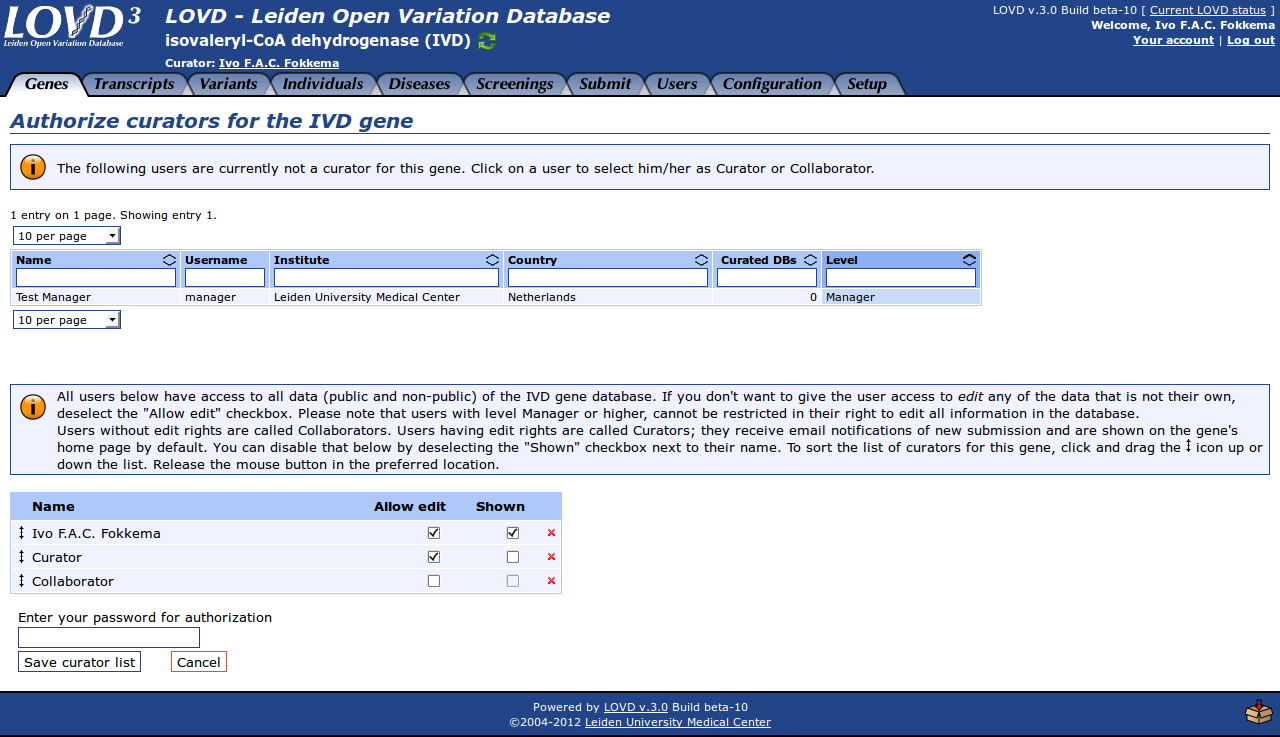
\includegraphics[width=\linewidth]{c05s05_screenshot_authorize_curators.png}}%
  \caption{%
    The ``Authorize curators'' form, with on the top the users who are available to be selected, and on the bottom the selected curators and collaborators.}
  \label{fig:c05s05_screenshot_authorize_curators}
  \end{shaded}
\end{figure}

On the top of the page, you see a listing of all available users in the system, whichever level they have.
Users that are already selected as curators or collaborators are shown in the bottom.
To add a user as a curator or collaborator, search for the user in the top user list, and click the user entry.
The user is then moved to the bottom.
\par
In the bottom table, you see two checkboxes for each user.
Also, you can sort the curators by dragging and dropping them in the list (see subsection \hyperlink{ssec:sorting_curators}{Sorting curators}).
The first checkbox indicates whether or not they are allowed to edit the data in this gene's database.
Users allowed to edit the data, are curators.
Unchecking this checkbox turns this user in a collaborator for this gene;
 he can still see all public and unpublic data in this gene database, but he can't edit it, like curators can.
If the user is to be a curator, he will receive notifications of variant data submissions and submission updates.
Collaborators do not receive such emails.

The second checkbox indicates whether or not the user's name and email address is
 shown on the gene homepage and on the top of every page while this gene is selected.
Curators can be hidden from the gene homepage and the page headers by unchecking this checkbox.
Collaborators are always hidden, it is therefore not possible to change the second checkbox while the first checkbox is unchecked.

To remove an user as a curator or collaborator, click the red cross at the far right side of the table.
You can only assign or remove curators if your user level is higher than that of the user you wish to assign/remove.
\vskip \baselineskip

Please note that managers and the database administrator can never be made collaborators, since disallowing them to edit data contradicts their user level.
They will always be allowed to edit all data in the system.
Selecting them as curators doesn't grant them additional access rights, but does enable the notification emails.

Also, please note that all genes in LOVD should have at least one visible curator.
To be able to successfully submit the ``Authorize curators'' form, there needs to be at least one user with the ``Allow edit'' and ``Shown'' checkboxes checked.



\hypertarget{ssec:sorting_curators}{}
\subsection{Sorting curators}

\begin{figure}[ht]
  \begin{shaded}
  \frame{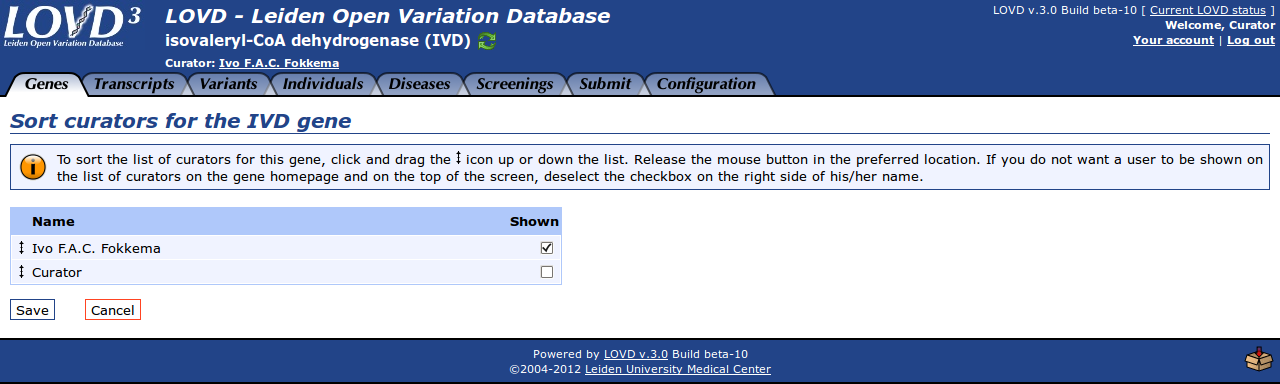
\includegraphics[width=\linewidth]{c05s05_screenshot_sort_curators.png}}%
  \caption{%
    The ``Sort curators'' form, allowing curators to resort the gene's list of curator names,
     and show or hide curators from the gene homepage and the page headers.}
  \label{fig:c05s05_screenshot_sort_curators}
  \end{shaded}
\end{figure}

\begin{wrapfigure}[3]{r}{8cm} % Only wrap for 3 lines
  \vspace{-25pt}
  \begin{leftbar}
    Required level: Curator\\
    Available from: LOVD 3.0 Build 01
  \end{leftbar}
\end{wrapfigure}
Since the curator names are shown on the gene homepage and on the page headers, it is sometimes necessary to sort the curator names in a specific order.
This can be done on the ``Authorize curators'' form (see figure \ref{fig:c05s05_screenshot_authorize_curators}
 on page \pageref{fig:c05s05_screenshot_authorize_curators}).
Curators, who don't have access to that form, use the ``Sort/hide curator names'' option from the ``Options'' dropdown menu on the gene homepage.
This form greatly resembles the bottom part of the ``Authorize curators'' form, allowing to sort and show or
 hide the curator names (see figure \ref{fig:c05s05_screenshot_sort_curators} on page \pageref{fig:c05s05_screenshot_sort_curators}).

\begin{wrapfigure}[3]{r}{5cm} % Only wrap for 3 lines
  \vspace{-25pt}
  \begin{framed}
    \raisebox{-0.5mm}{
\includegraphics[width=1.5mm]{drag_vertical.png}} Drag/sort handle
  \end{framed}
\end{wrapfigure}
To resort the list of curators, move your mouse over the drag handle (see figure) on the left
 of the curator name, and click and drag the name up or down the list.
Release the mouse button in the preferred location.
Don't forget to click the ``Save'' button to save the new sort order!
\clearpage % Makes the hyper target actually point to the right place.










\hypertarget{chap:transcripts}{}
\chapter{Gene transcripts}
LOVD3 handles transcripts very differently from LOVD2.
In LOVD3, configuring at least one transcript for a certain gene is necessary to be able to add variant data to the gene database.
Genomic variants can always be added, but to record the effect of a variant on a certain gene, that gene must have at least one transcript defined.
As a source for transcript information, LOVD relies on Mutalyzer, which gathers transcript information from different sources.
Therefore, it is possible that new transcripts recently included in the NCBI database, are not yet available in LOVD because
 either the NCBI hasn't rebuilt its mapping database yet, or Mutalyzer didn't pick up the new mapping information yet.
LOVD3 does not restrict you in the number of transcripts you can configure per gene, but note that for each transcript added,
 each variant gains more data fields that need to be filled in by the submitter, so make sure that the additional transcripts are actually needed.





\section{Which transcript(s) should I pick?}
In principle, we suggest using the predominant transcript, especially if only changes in this transcript cause a change in phenotype.
Otherwise we recommend using the longest transcript (i.e., the transcript resulting in the longest protein).
Using the predominant transcript makes confirmation of the variant effect on RNA level easier and
 usually the variant numbering on this transcript will be most familiar with other research groups.
Using the longest transcript has the advantage of being able to annotate all exonic variants with a (predicted) effect on protein level.
\vskip \baselineskip

As said, LOVD3 allows you to use more than one transcript per gene.
Good examples that justify using multiple transcripts in LOVD, is when different transcripts are expressed in different tissues,
 when changes in different transcripts cause different phenotypes, or when different research groups focus on different transcripts
 (for example, when no transcript is availabile that contains all exons).





\section{Creating new transcripts}
\begin{wrapfigure}[3]{r}{8cm} % Only wrap for 3 lines
  \vspace{-25pt}
  \begin{leftbar}
    Required level: Curator\\
    Available from: LOVD 3.0 Build 01
  \end{leftbar}
\end{wrapfigure}
The simplest way to create a gene transcript in LOVD, is to select it when \hyperlink{sec:gene_create}{creating a gene database}.
However, if you'd like to add more transcripts later, please proceed to the \hyperlink{sec:gene_homepage}{gene homepage}.
Click on the ``Options'' menu button to open up the gene entry's menu.
If you do not see the ``Options'' menu button, you are not logged in or you do not have rights to edit this gene's settings.
In the opened menu, click ``Add transcript(s) to gene'' to open up the gene's edit form.
Please wait while we contact Mutalyzer to provide a list of available transcripts.
If you get the error message ``No more transcripts available that have not been added yet!'',
 then all transcripts that are available to Mutalyzer have already been added to this gene.

Select the transcript(s) you would like to add, and click the button ``Add transcript(s) to gene''.
After the confirmation, you will be forwarded to the gene homepage.
Beneath the header ``Active transcripts'' you can see which transcripts are now active.





\section{Editing a transcript}
\begin{wrapfigure}[3]{r}{8cm} % Only wrap for 3 lines
  \vspace{-25pt}
  \begin{leftbar}
    Required level: Curator\\
    Available from: LOVD 3.0 Build 01
  \end{leftbar}
\end{wrapfigure}
Because LOVD standardizes the transcript information, there is very little information that is freely editable.
At this moment, you are only allowed to assign or change Ensembl identifyers to the transcript(s) you use.
To edit a certain transcript, proceed to the gene homepage, scroll down to ``Active transcripts'' and click the transcript in question.
Alternatively, click the ``Transcripts'' tab from anywhere in LOVD.
If you already had a gene database selected, you now see the transcripts active in this gene and you can click one to view its details.
If you did not have a gene database selected, you now see all transcripts in the database.
Use the filtering boxes to find the transcript you are looking for, and click it to view its details.
\vskip \baselineskip

Click on the ``Options'' menu button to open up the transcript entry's menu.
If you do not see the ``Options'' menu button, you are not logged in or you do not have rights to edit this transcript's settings.
In the opened menu, click ``Edit transcript information'' to open up the transcript's edit form.



\subsection{General information}
This part contains IDs to other sources, to aid in data exchange.
\begin{description}
  \item[Transcript Ensembl ID] \hfill \\
  If this transcript is also known in Ensembl, enter its Ensembl ENST ID here.
  \item[Protein Ensembl ID] \hfill \\
  If this transcript's protein product is also known in Ensembl, enter its Ensembl ENSP ID here.
  \item[Protein Uniprot ID] \hfill \\
  If this transcript's protein product has an Uniprot ID, enter it here.
\end{description}





\section{Deleting a transcript}
\begin{wrapfigure}[3]{r}{8cm} % Only wrap for 3 lines
  \vspace{-25pt}
  \begin{leftbar}
    Required level: Curator\\
    Available from: LOVD 3.0 Build 01
  \end{leftbar}
\end{wrapfigure}
Deleting a transcript removes all information related to the transcript in question from all variants in the database.
Just like when \hyperlink{sec:gene_delete}{deleting a gene}, this \emph{does not remove the genomic variants from the database!}
From the transcript's detailed view, click on the ``Options'' menu button to open up the transcript's menu, and select the ``Delete transcript entry'' option.
On the next page, confirm by typing your password in the input box and submit the form to complete the removal.










\chapter{Custom columns}
To make sure LOVD can be used by a great variety of users who all focus on storing different data,
 LOVD allows great flexibility in the form of \emph{custom columns}; data fields that can be personalized by the curators,
 or even completely newly defined.
All standard LOVD columns can be edited and removed, except for the HGVS recommended columns,
 which can only be edited but not removed.
Besides this default set of selected columns which are added by default,
 LOVD also comes with a set of columns that have not been added to the data tables yet,
 but can be added with a click of a button.
Additional columns can be created to suit your every need.





\hypertarget{sec:custom_column_categories}{}
\section{Custom column categories}
\label{sec:custom_column_categories}
In LOVD3, custom columns come in five different categories.
\begin{description}
  \item[Individual] \hfill \\
  Information on the individual, not related to disease, not changing over time, such as date of birth, geographic or ethnic origin.
  \item[Phenotype] \hfill \\
  Information on the phenotype, related to disease, possibly changing over time, such as blood pressure, body length or date seen by specialist.
  \item[Screening] \hfill \\
  Information on the detection of new variants, such as detection technique, laboratory conditions or type of sample taken from the individual.
  \item[Variant On Genome] \hfill \\
  Information on the variant(s) found, in general or on the genomic level, such as restriction site change, DNA change on genomic level, or reference describing the variant.
  \item[Variant On Transcript] \hfill \\
  Information on the variant(s) found, specific for the transcript level, such as predicted effect on protein level, DNA change on mRNA level, or exon number.
\end{description}

Of these five different categories, two are \emph{shared}: they can be turned on or off by curators for specific diseases or genes, their so-called \emph{parent objects}.
Some of these columns' settings can also be changed per parent object they are enabled in.
The two shared custom column types are ``Phenotype'', configurable per disease, and ``Variant On Transcript'', configurable per gene.
\vskip \baselineskip

The other three categories are system-wide; meaning they are either \emph{always} on (enabled), or \emph{always} off (disabled).
These column are referred to as \emph{non-shared} columns, and can only be enabled, disabled and managed by Manager level users, or the Database administrator.
The three non-shared custom column types are ``Individual'', ``Screening'' and ``Variant On Genome''.





\pagebreak[4] % Break the page here (up to 4; 4 is very persistent)
\hypertarget{sec:custom_column_create}{}
\section{Creating a new custom column}
\label{sec:custom_column_create}
\begin{wrapfigure}[3]{r}{8cm} % Only wrap for 3 lines
  \vspace{-25pt}
  \begin{leftbar}
    Required level: Manager\\
    Available from: LOVD 3.0 Build 01
  \end{leftbar}
\end{wrapfigure}
By creating a new custom column, you can define what kind of information you want to store in the database.
Please note that \emph{defining} this type of information, does not automatically make LOVD \emph{store} this information.
You will need to enable the column after defining it, so it actually gets added to the data entry form and show up in the data tables.
\vskip \baselineskip

To create a new custom column, click on the ``Create new custom data column'' option from the ``Setup'' tab dropdown menu,
 or the ``Create new custom data column'' link in the setup area.
Firstly, you will need to choose which type of column you would like to create.
For more information on the different column types, see the \hyperlink{sec:custom_column_categories}{previous section}.
Please note that you can never change the type of a column once it has been chosen.
Select the type of column you would like to create, by clicking its description.
You are then forwarded to the entry form specific for this type of custom column.



\subsection{Column name and descriptions}
Here the description of the new column is defined; its displayed name and the explanation of its contents to the users.
\begin{description}
  \item[Column ID] \hfill \\
  Choose a simple unique name for your column, consisting of only letters, numbers and underscores.
  Subcategories must be divided by a slash (/), such as ``Geographic\_origin\slash Country'',
   ``Blood\_pressure/Systolic'', ``Protocol/Date\_updated'', ``Frequency/dbSNP'' or ``Protein/Codon''.
  \item[Column heading] \hfill \\
  This will appear above the column in data tables and on the legend.
  In principle, this is free text, but try to keep it short, because a long name will increase the width of the column.
  \item[Description on short legend] (HTML enabled)\hfill \\
  \emph{For shared columns, this value can be changed separately for each parent object this column has been added to.}
  \\
  Describe the meaning of the column in short.
  This will appear when a user moves his mouse over the column header in the data tables.
  \item[Description on full legend] (HTML enabled)\hfill \\
  \emph{For shared columns, this value can be changed separately for each parent object this column has been added to.}
  \\
  Describe the meaning of the column.
  You can be very elaborate here.
  This text will be shown on the full legend of the data table.
\end{description}



\subsection{Data and form settings}
Here you define what the column looks like on the data entry form, and what kind of data it will store.
There are two ways to define the data type of your custom column.
The recommended way is to use the data type wizard, which will fill in the MySQL and the form type values.
Only if you really know what you're doing, you can edit the MySQL data type and the form type directly.
Its formats are out of the scope of this manual, and therefore not explained here.

\subsubsection{Using the data type wizard}
To start the data type wizard, click the ``Start data type wizard'' button.
The wizard will open in a new window.

Firstly, you need to select what type of data entry field you want to create for your custom column.
In the ``Basic form style'' field, choose from one of these options:
\begin{description}
  \item[Text/numeric input field] \hfill \\
  A standard input field allowing textual or numerical free text input.
  \item[Integer input field] \hfill \\
  A standard input field, visually similar to the text/numeric input field, but allowing only whole numbers to be filled in.
  \item[Decimal input field] \hfill \\
  A standard input field, visually similar to the text/numeric input field, but allowing only numbers with a configurable number of decimals.
  \item[Large multi-row textual input field] \hfill \\
  A large text field with multiple rows, allowing large amounts of text to be filled in.
  \item[Drop down list (one option selected)] \hfill \\
  A drop down list with a set of options of which the user must choose one value.
  \item[Selection list (multiple options selected)] \hfill \\
  A selection list where the user can select one or more options or ranges.
  \item[Date input field] \hfill \\
  A standard input field, visually similar to the text/numeric input field, but allowing only dates (year, month, day), optionally also storing time (hours, minutes, seconds).
  The input format is YYYY-MM-DD or YYYY-MM-DD HH:MM:SS.
  \item[On/off checkbox] \hfill \\
  A simple checkbox allowing only a yes/no answer.
\end{description}

\noindent
Select the wanted data entry type and click ``Next \guillemotright''.

\vskip 1cm

\noindent
The next page shows you some additional options that depend on the type of field you've chosen.
\begin{description}
  \item[Column name on form] (all field types)\hfill \\
  The name the column will have on the data entry form.
  This is usually the same as the ``Column heading'' field.
  \item[Help text] (all field types)\hfill \\
  If you think the data field needs clarification for users, especially those who don't know this field well, add such clarification here.
  By filling in this field, LOVD will add a question mark icon next to the field on the data entry form.
  When the user moves his mouse over the question mark icon, the text entered here is shown.
  Since the text is shown as a highlight, it does not disrupt the structure of the data entry form, so feel free to type lengthy texts.
  \item[Notes on form] (all field types, HTML enabled)\hfill \\
  \emph{For shared columns, this value can be changed separately for each parent object this column has been added to.}
  \\
  If you think the data field needs clarification for all users, add such clarification here.
  The text given here will be shown directly underneath the data entry field.
  Therefore, keep it short, since long texts will make the data entry form very long.
  \item[Width on form (characters)] (all input fields and text area)\hfill \\
  The input field width on the form, in number of characters.
  \item[Height on form (lines)] (text area and multiple selection list)\hfill \\
  The height of your field on the data entry form, in lines.
  For multiple selection lists, this implies the number of options visible at the same time.
  \item[Maximum input length (characters)] (text and integer input field types)\hfill \\
  The maximum number of characters allowed the be filled in.
  If a user tries to enter more characters in your field, an error is issued.
  For the integer input type, this implies the maximum value that can be filled in.
  \item[Number of digits before the decimal point] (decimal field only)\hfill \\
  The maximum number of digits allowed before the decimal point.
  This practically limits the maximum value of the field.
  \item[Number of digits following the decimal point] (decimal field only)\hfill \\
  The maximum number of digits allowed at the right of the decimal point.
  This limits the maximum precision of values in the field.
  \item[Regular expression pattern] (text input only)\hfill \\
  For advanced users only.
  You can enter a full regular expression pattern (PHP's Perl-compatible regular expression syntax), including `/' delimiters and possible modifiers.
  Using this, you can force a certain format for the input.
  Make sure it's valid, otherwise you risk getting all this column's data input rejected.
  \item[Allow only positive values] (integer and decimal fields)\hfill \\
  Select this to allow only positive numbers to be entered.
  \item[Provide ``-- select --'' option] (drop down list only)\hfill \\
  This will add an option named ``-- select --'' to the list of options, that will be selected by default and will be regarded as an empty value.
  If this option is not set, the first option of the list will be the default selected option.
  \item[Provide ``select all'' link] (multiple selection list only)\hfill \\
  This will add a link next to the selection list that allows the user to instantly select all available options.
  \item[List of possible options] (both list types)\hfill \\
  \emph{For shared columns, this value can be changed separately for each parent object this column has been added to.}
  \\
  Enter the options available for this field, one options per line.
  If you want to use abbreviations, use: Abbreviation = Long name, like ``DMD = Duchenne Muscular Dystrophy''.
  In that case the user will see the long name in the selection list, but the abbreviation will be stored in the database.
  \item[Also store time?] (date field only)\hfill \\
  Select this to also store time (hours, minutes, seconds) in this date field.
  \item[Default value] (all input fields except text area)\hfill \\
  A default value that will appear in the field when creating a new data entry.
\end{description}

\noindent
Click the ``Finish'' button to have the data type wizard fill in the ``MySQL data type'' and ``Form type'' fields for you,
 based on the information you provided.



\subsection{Column settings}
Here you can change some of the column's settings.
For shared columns (see section ``\hyperlink{sec:custom_column_categories}{\nameref{sec:custom_column_categories}}''),
 most of these settings can also be changed per parent object where this column has been added to.
\begin{description}
  \item[Include this column for newly configured genes/diseases] (shared columns only)\hfill \\
  When this is selected, new genes (for VariantOnTranscript columns) or diseases (for Phenotype columns) will have this custom column enabled by default.
  When you leave this off, the curators of new genes or diseases will have to enable the column themselves, should they want to use it.
  \item[Column display width in pixels] \hfill \\
  \emph{For shared columns, this value can be changed separately for each parent object this column has been added to.}
  \\
  Here you can define how wide the column should be in data listings.
  This is measured in pixels.
  Since the width depends on the screen's resolution, a hint is provided how wide the currently selected width is on the current screen.
  \item[Mandatory field] \hfill \\
  \emph{For shared columns, this value can be changed separately for each parent object this column has been added to.}
  \\
  With this option selected, users can't leave this column empty.
  \item[Show contents to public] \hfill \\
  \emph{For shared columns, this value can be changed separately for each parent object this column has been added to.}
  \\
  This controls whether or not users with no specific authorization on the data entry can see the contents of this column.
  \item[Show field on submission form] \hfill \\
  \emph{For shared columns, this value can be changed separately for each parent object this column has been added to.}
  \\
  If you don't want submitters to fill in this column, but reserve the use for curators, disable this checkbox.
  Please note that unsetting this will not hide the contents of the column from the public, it merely stops them from entering data in it.
% IMPLEMENT
%Include in search form: This option controls whether or not this column shows on the special search overview that allows the public to find the number of entries in the database (including hidden entries) matching one or more search terms on a specified set of columns.
\end{description}



\subsection{Link settings}
Here you can select which custom links will be active in this custom column.
% For more information on custom links, see.....
\begin{description}
  \item[Active custom links] \hfill \\
  Select any number of custom links, or leave all unselected if you do not wish to use custom links in this field.
  Note that the use of custom links only makes sense for fields that accept text input.
\end{description}

\noindent
Enter your password at the bottom of the form and submit it.
Your custom column is now created, and you can choose to enable the column if you wish.
Also, you might want to check the \hyperlink{sec:columns_order}{column order}, since newly created custom columns are appended to be the last column.





\section{Enabling custom columns}
Directly after creating a new custom column, or at any later time, you can enable a custom column.
It must already exist in the database, otherwise you first need to \hyperlink{sec:custom_column_create}{create it}.
\emph{Non-shared} custom columns (Individual, Screening and Variant On Genome categories) are enabled system-wide, which requires manager access.
\emph{Shared} custom columns (Phenotype and Variant On Transcript categories) can be enabled by parent-object (disease or gene, respectively) and require curator access.



\subsection{Enabling non-shared custom columns}
\begin{wrapfigure}[3]{r}{8cm} % Only wrap for 3 lines
  \vspace{-25pt}
  \begin{leftbar}
    Required level: Manager\\
    Available from: LOVD 3.0 Build 01
  \end{leftbar}
\end{wrapfigure}
The non-shared, system-wide custom column types are Individual, Screening and Variant On Genome.
To enable a non-shared custom column, you should start from the list of currently available columns.
% This text is also used for disabling custom columns.
You can get there in two ways:
\begin{itemize}
  \item Depending on which type of column you wish to enable,
   click the ``Enable more custom columns'' link in the ``Individuals'' or ``Screenings'' menu tabs' dropdown menu,
   or the ``Enable more genomic custom columns'' link from the ``Variants'' menu tab dropdown menu.
  \item Click the ``Browse all custom data columns'' link of the setup menu tab dropdown menu, or from the setup area,
   click the ``Browse all custom data columns already available to enable or disable them, or view or edit their settings'' link listed under ``Custom data columns''.
  This is the list of all custom columns.
  To filter this list for category, click the options wheel icon on the top left hand side of the columns listing to open up the menu, and select the category you are interested in.
  You can also filter for category by typing (part of) the name in the ``Category'' column filter box, and press the ``Enter'' key.
% Until here.
  To further filter the list for columns not yet added to the data table, fill in a zero (`0') in the ``Active'' column filter box and press the ``Enter'' key.
\end{itemize}
From the column overview, click the column you wish to enable.
\vskip \baselineskip

In the detailed view of the custom column, you can review all the column's settings to verify that it suits your needs.
Click the ``Options'' menu button to open up the column's menu, and click on ``Enable column''.
Please note that when your database already contains a lot of information, enabling a new non-shared column may take some time.
If this is the case, LOVD will display a warning.
Type in your password in the ``Enter your password for authorization'' field for verification of your authorization, and submit the form.
The column is now enabled and visible in the data entry forms and the data listings and detailed views.
You may want to review or \hyperlink{ssec:columns_order_system-wide}{change the order of the custom columns} now.



\subsection{Enabling shared custom columns}
\begin{wrapfigure}[3]{r}{8cm} % Only wrap for 3 lines
  \vspace{-25pt}
  \begin{leftbar}
    Required level: Curator\\
    Available from: LOVD 3.0 Build 01
  \end{leftbar}
\end{wrapfigure}
The shared custom column types are Phenotype and Variant On Transcript.
Before enabling more shared columns, you might first want to check out the default order in which they will appear.
To change the default order for shared custom columns, see subsection ``\hyperlink{ssec:columns_order_system-wide}{Changing the system-wide custom column order}''.

To enable a shared custom column, you should start from the list of currently available columns.
You can get there in two ways:
\begin{itemize}
  \item From any disease or gene that you have authorization of, open the ``Options'' menu button and click the
   ``View all available phenotype columns'' or ``View all available variant columns'' link, depending on which type of column you wish to enable.
  % This text is copied below.
  \item If you're a manager or higher, click the ``Browse all custom data columns'' link of the setup menu tab dropdown menu, or from the setup area,
     click the ``Browse all custom data columns already available to enable or disable them, or view or edit their settings'' link listed under ``Custom data columns''.
    This is the list of all custom columns.
    To filter this list for category, click the options wheel icon on the top left hand side of the columns listing to open up the menu, and select the category you are interested in.
    You can also filter for category by typing (part of) the name in the ``Category'' column filter box, and press the ``Enter'' key.
\end{itemize}
Please note that in this custom column overview, the ``Active'' field simply states whether or not this column has been added to the data table, i.e. is active for \emph{any} parent object.
\\
From the column overview, click the column you wish to enable.
\vskip \baselineskip

In the detailed view of the custom column, you can review all the column's settings to verify that it suits your needs.
Click the ``Options'' menu button to open up the column's menu, and click on ``Enable column''.
Please note that if this shared custom column was not active yet and your database already contains a lot of information, enabling this column may take some time.
If this is the case, LOVD will display a warning.
From the ``Add this column to'' selection list, select the parent objects (diseases or genes) you wish to enable this column for.
For help on how to use this type of selection list, move your mouse over the blue help icon.
If the parent object you are looking for is not shown in this list, you have no authorization on the object to change its column's settings.

Finally, type in your password in the ``Enter your password for authorization'' field for verification of your authorization, and submit the form.
The column is now enabled and visible in the data entry forms and the data listings and detailed views.
To make sure the column ended up in the right order between the already enabled ones,
 you may want to review or \hyperlink{ssec:columns_order_shared}{change the object-specific order of shared custom columns}.





\section{Editing custom column settings}
Shared columns have some settings, mostly related to the display of the column, which can be set per parent object (a certain disease or gene).
We will refer to these settings as \emph{object-specific settings}.
All other settings are system-wide and can only be performed by a manager or higher.
Non-shared columns only have system-wide settings and can not be configured per disease or gene.



\subsection{Editing system-wide custom column settings}
\begin{wrapfigure}[3]{r}{8cm} % Only wrap for 3 lines
  \vspace{-25pt}
  \begin{leftbar}
    Required level: Manager\\
    Available from: LOVD 3.0 Build 01
  \end{leftbar}
\end{wrapfigure}
Both shared and non-shared columns have sys\-tem-wide settings that can be changed by a manager or higher.
However, the way these columns respond to changes to the system-wide settings are not the same.
For non-shared columns, each change to the system-wide settings will be effective immediately.
For shared columns, only the settings that are not \emph{object-specific} (see above) are effective immediately.
All changes to object-specific settings however, come to serve as new default values for when the custom column in question is activated for new genes or diseases.
Already enabled shared custom columns will not have their object-specific settings reset, unless they are explicitly reset to the (new) default settings (described in the paragraph below).
\vskip \baselineskip

To edit a custom column's system-wide settings, you should start from the list of currently available columns.
% This text is copied above.
Click the ``Browse all custom data columns'' link of the setup menu tab dropdown menu, or from the setup area,
 click the ``Browse all custom data columns already available to enable or disable them, or view or edit their settings'' link listed under ``Custom data columns''.
This is the list of all custom columns.
To filter this list for category, click the options wheel icon on the top left hand side of the columns listing to open up the menu, and select the category you are interested in.
You can also filter for category by typing (part of) the name in the ``Category'' column filter box, and press the ``Enter'' key.
% Until here.
Now, click the column which settings you wish to edit.
Click the ``Options'' menu button to open up the column's menu, and click on ``Edit custom data column settings''.

The form to edit the system-wide settings is equal to the form used to create a new custom column, with two exceptions.
The ``Column ID'' field is not present here, since you can not change a column's ID once you created it.
Also, for shared columns, at the bottom of the form a checkbox is present labeled ``Apply changes to all genes/diseases where this column is active''.
Checking this checkbox effectively resets all enabled instances of the column and applies all changes you make on this form to them, overwriting possible modifications of object-specific settings.
All other fields on this form are explained in the section ``\hyperlink{sec:custom_column_create}
 {\nameref{sec:custom_column_create}}''.



\subsection{Editing object-specific (shared) custom column settings}
\begin{wrapfigure}[3]{r}{8cm} % Only wrap for 3 lines
  \vspace{-25pt}
  \begin{leftbar}
    Required level: Curator\\
    Available from: LOVD 3.0 Build 01
  \end{leftbar}
\end{wrapfigure}
The object-specific settings, editable per gene or disease, are (also see section ``\hyperlink{sec:custom_column_create}
 {\nameref{sec:custom_column_create}}''):
\tightlists
\begin{itemize}
  \item Description on short legend
  \item Description on full legend
  \item Notes on form
  \item List of possible options (for selection list type columns)
  \item Column display width in pixels
  \item Mandatory field
  \item Show contents to public
  \item Show field on submission form
\end{itemize}
\defaultlists
\vspace{\baselineskip}
% Copied this text to below.
To change these settings, first you need to proceed to the detailed view of the disease or gene in question.
For Phenotype columns, move your mouse over the ``Diseases'' menu tab, and click the ``View all diseases'' link from the dropdown menu.
For Variant On Transcript columns, move your mouse over the ``Genes'' menu tab, and click the ``View all genes'' link from the dropdown menu.
Then, select the parent object you would like to change the object-specific settings for.

From the parent object's detailed view, open the ``Options'' menu and click the ``View enabled phenotype columns'' or ``View enabled variant columns'' link.
From the list of enabled columns, click the one you wish to edit the settings for.
Open up the ``Options'' menu and then click ``Edit settings for this disease only'' for Phenotype columns, or ``Edit settings for this gene only'' for Variant On Transcript columns.
For explaination of the available fields, please see the section ``\hyperlink{sec:custom_column_create}
 {\nameref{sec:custom_column_create}}''.
After submitting the form, the changes are effective immediately, but applied to the chosen parent object only.





\pagebreak
\hypertarget{sec:columns_order}{}
\section{Changing the order of custom columns}
Custom columns are shown in a predefined, but adaptable order.
This order determines how custom columns are shown in the data tables, in the download files, and on data entry forms.
It is therefore important that the columns are sorted in a sensible order.

Just like the custom column settings, shared columns can have an object-specific order, different from the default order.
Similarly, the order of non-shared columns is system-wide and needs to be configured by a manager or up.
\vskip \baselineskip

Please note that columns from different categories can not be mixed.
% FIXME: add link to info on the overview?
Some data listings show overviews of different types of data joined together, such as variants on genomic level joined with the variant's effect on transcript level.
In this case, the columns representing genomic data, such as chromosome, DNA description on genomic level and the allele field,
 can not be mixed with columns representing data related to the change on the transcript, such as exon number, DNA description on the transcript level or the effect on protein level.
Only the order in which each category's columns are shown, can be changed.



\hypertarget{ssec:columns_order_system-wide}{}
\subsection{Changing the system-wide custom column order}
\begin{wrapfigure}[3]{r}{8cm} % Only wrap for 3 lines
  \vspace{-25pt}
  \begin{leftbar}
    Required level: Manager\\
    Available from: LOVD 3.0 Build 01
  \end{leftbar}
\end{wrapfigure}
For non-shared columns, changing the system-wide custom column order will effectively change the current order in which they are shown in data listings and data entry forms.
For shared columns, changing the system-wide order will merely change the default order in which the columns appear when new parent objects (diseases, genes) are created.
It also influences where a newly enabled column will show up amidst the columns already active for the object it just got added to.
The order of already enabled shared custom columns will not be affected.
\vskip \baselineskip

To change the custom column's system-wide order, you should start from the list of currently available columns.
% This text is copied above.
Click the ``Browse all custom data columns'' link of the setup menu tab dropdown menu, or from the setup area,
 click the ``Browse all custom data columns already available to enable or disable them, or view or edit their settings'' link listed under ``Custom data columns''.
This is the list of all custom columns.
To filter this list for category, click the options wheel icon on the top left hand side of the columns listing to open up the menu, and select the category you are interested in.
% Until here.
Now, click the options wheel icon again, and click the ``Change order of columns'' link.
Alternatively, first select one of the columns from the selected category,
 and on the detailed view open the ``Options'' menu and click the ``Re-order all \guillemotleft\emph{category}\guillemotright\ columns'' link.
\vskip \baselineskip

\begin{wrapfigure}[3]{r}{5cm} % Only wrap for 3 lines
  \vspace{-25pt}
  \begin{framed}
    \raisebox{-0.5mm}{
\includegraphics[width=1.5mm]{drag_vertical.png}} Drag/sort handle
  \end{framed}
\end{wrapfigure}
You now see all custom columns in this category, both active and not active.
On the left of each column's header you see a handle (see figure) to drag the column up or down.
To change the order in which the columns are shown, move your mouse over the drag handle, and click and drag the name up or down the list.
Release the mouse button where you wish to drop the column.
Don't forget to click the ``Save'' button to save the new sort order!



\pagebreak
\hypertarget{ssec:columns_order_shared}{}
\subsection{Changing the object-specific order of shared custom columns}
\begin{wrapfigure}[3]{r}{8cm} % Only wrap for 3 lines
  \vspace{-25pt}
  \begin{leftbar}
    Required level: Curator\\
    Available from: LOVD 3.0 Build 01
  \end{leftbar}
\end{wrapfigure}
When a new gene or disease is created, the current system-wide order of Variant On Transcript or Phenotype columns respectively, is copied and becomes this object's order of columns.
Curators and up can change this order, for instance when a new column has been enabled, since newly enabled columns are very likely to end up as the last column which may not be desired.

% Copied this text from above.
To change the order, first you need to proceed to the detailed view of the disease or gene in question.
For Phenotype columns, move your mouse over the ``Diseases'' menu tab, and click the ``View all diseases'' link from the dropdown menu.
For Variant On Transcript columns, move your mouse over the ``Genes'' menu tab, and click the ``View all genes'' link from the dropdown menu.
Then, select the parent object you would like to change the order of the custom columns of.

From the parent object's detailed view, open the ``Options'' menu and click the ``Re-order enabled phenotype columns'' or ``Re-order enabled variant columns'' link.
Alternatively, click the ``View enabled phenotype columns'' or ``View enabled variant columns'' link from the menu,
 and on the page that follows open the ``Options'' menu to click the ``Change order of columns'' link.
\vskip \baselineskip

\begin{wrapfigure}[3]{r}{5cm} % Only wrap for 3 lines
  \vspace{-25pt}
  \begin{framed}
    \raisebox{-0.5mm}{
\includegraphics[width=1.5mm]{drag_vertical.png}} Drag/sort handle
  \end{framed}
\end{wrapfigure}
You now see the enabled columns for the selected parent object, with on the left of each column's header a handle (see figure) to drag the column up or down.
To change the order in which the columns are shown, move your mouse over the drag handle, and click and drag the name up or down the list.
Release the mouse button where you wish to drop the column.
Don't forget to click the ``Save'' button to save the new sort order!





\hypertarget{sec:columns_disable}{}
\section{Disabling custom columns}
Custom columns that you no longer wish to use, can in most circumstances be removed by disabling the column.
Exceptions in this case are \emph{HGVS standard} columns.
HGVS standard custom columns are columns that are part of the mandatory minimal data set as defined by the HGVS for Locus-Specific DataBases (LSDBs).
This is to preserve the minimal quality of the data within the database, and LOVD will not allow you to remove these columns.
Disabling non-shared custom columns is a system-wide change, which requires manager access.
Disabling shared custom columns can be done per parent-object and requires curator access.



\subsection{Disabling non-shared custom columns}
\begin{wrapfigure}[3]{r}{8cm} % Only wrap for 3 lines
  \vspace{-25pt}
  \begin{leftbar}
    Required level: Manager\\
    Available from: LOVD 3.0 Build 01
  \end{leftbar}
\end{wrapfigure}
To disable a non-shared custom column, you should start from the list of currently active columns.
% This text is also used for enabling custom columns.
You can get there in two ways:
\begin{itemize}
  \item Depending on which type of column you wish to disable,
   click the ``View active custom columns'' link in the ``Individuals'' or ``Screenings'' menu tabs' dropdown menu,
   or the ``View active genomic custom columns'' link from the ``Variants'' menu tab dropdown menu.
  \item Click the ``Browse all custom data columns'' link of the setup menu tab dropdown menu, or from the setup area,
   click the ``Browse all custom data columns already available to enable or disable them, or view or edit their settings'' link listed under ``Custom data columns''.
  This is the list of all custom columns.
  To filter this list for category, click the options wheel icon on the top left hand side of the columns listing to open up the menu, and select the category you are interested in.
  You can also filter for category by typing (part of) the name in the ``Category'' column filter box, and press the ``Enter'' key.
% Until here.
  To further filter the list for columns currently enabled, fill in a one (`1') in the ``Active'' column filter box and press the ``Enter'' key.
\end{itemize}
From the column overview, click the column you wish to disable.
\vskip \baselineskip

Click the ``Options'' menu button to open up the column's menu, and click on ``Disable column and remove values''.
Please note that when your database already contains a lot of information, disabling a non-shared column may take some time.
If this is the case, LOVD will display a warning.
Type in your password in the ``Enter your password for authorization'' field for verification of your authorization, and submit the form.
The column is now disabled and removed from the data entry forms and the data listings and detailed views.

If the ``Disable column and remove values'' link is not enabled, i.e.\ you see it, but you can't click it, the column is an HGVS standard column, and it can not be removed.



\subsection{Disabling shared custom columns}
\begin{wrapfigure}[3]{r}{8cm} % Only wrap for 3 lines
  \vspace{-25pt}
  \begin{leftbar}
    Required level: Curator\\
    Available from: LOVD 3.0 Build 01
  \end{leftbar}
\end{wrapfigure}
Shared custom columns can be disabled for one parent object only, or from multiple parent objects at the same time.
\vskip \baselineskip

To disable the given column \emph{for one parent object only}, proceed to the detailed view of this parent object (disease or gene).
Then, open the ``Options'' menu button and click the ``View enabled phenotype columns'' or ``View enabled variant columns'' link, depending on the type of column you wish to disable.
Click the column, then from its ``Options'' menu button, select ``Remove column from this disease'' or ``Remove column from this gene'', depending on the type of column.
Please note that if this shared custom column will no longer be active for any parent object and your database already contains a lot of information, disabling this column may take some time.
If this is the case, LOVD will display a warning.
Type in your password in the ``Enter your password for authorization'' field for verification of your authorization, and submit the form.

If the ``Remove column'' link is not enabled, i.e.\ you see it, but you can't click it, the column is an HGVS standard column, and it can not be removed.
\vskip \baselineskip

To disable the given column \emph{for multiple parent objects at the same time}, start with one of the following steps.
\begin{itemize}
  \item From any disease or gene that you have authorization of, open the ``Options'' menu button and click the
   ``View all available phenotype columns'' or ``View all available variant columns'' link, depending on which type of column you wish to disable.
  \item If you're a manager or higher, click the ``Browse all custom data columns'' link of the setup menu tab dropdown menu, or from the setup area,
     click the ``Browse all custom data columns already available to enable or disable them, or view or edit their settings'' link listed under ``Custom data columns''.
    This is the list of all custom columns.
    To filter this list for category, click the options wheel icon on the top left hand side of the columns listing to open up the menu, and select the category you are interested in.
    You can also filter for category by typing (part of) the name in the ``Category'' column filter box, and press the ``Enter'' key.
\end{itemize}
To further filter the list for columns currently enabled, fill in a one (`1') in the ``Active'' column filter box and press the ``Enter'' key.
Please note that in this custom column overview, the ``Active'' field simply states whether or not this column has been added to the data table, i.e. is active for \emph{any} parent object.
\\
From the column overview, click the column you wish to disable.
\vskip \baselineskip

In the detailed view of the custom column, open its ``Options'' menu button, then select ``Disable column''.
Please note that if this shared custom column will no longer be active for any parent object and your database already contains a lot of information, disabling this column may take some time.
If this is the case, LOVD will display a warning.
From the ``Remove this column from'' selection list, select the parent objects (diseases or genes) you wish to remove this column from.
For help on how to use this type of selection list, move your mouse over the blue help icon.
If the parent object you are looking for is not shown in this list, you have no authorization on the object to change its column's settings.
Finally, type in your password in the ``Enter your password for authorization'' field for verification of your authorization, and submit the form.
The column is now disabled and removed from the data entry forms and the data listings and detailed views.

If the ``Disable column'' link is not enabled, i.e.\ you see it, but you can't click it, the column is an HGVS standard column, and it can not be removed.





\section{Deleting custom columns}
\begin{wrapfigure}[3]{r}{8cm} % Only wrap for 3 lines
  \vspace{-25pt}
  \begin{leftbar}
    Required level: Manager\\
    Available from: LOVD 3.0 Build 01
  \end{leftbar}
\end{wrapfigure}
Custom columns, which are created by users (managers or the database administrator), can also be deleted permanently from the system,
 for instance if they were for testing purposes only or if they are no longer needed.
First, you need to make sure the column is no longer active.
See section ``\hyperlink{sec:columns_disable}{Disabling custom columns}'' on how to inactivate a column.
\vskip \baselineskip

First, proceed to the column's detailed view; access the custom data columns listing through the setup menu tab dropdown menu or setup area,
 find the column you wish to delete, and click on its entry.
Then, from its ``Options'' menu button, select ``Delete column''.
Type in your password in the ``Enter your password for authorization'' field for verification of your authorization, and submit the form.

If the ``Delete column'' link is not enabled, i.e.\ you see it, but you can't click it, the column is either still active (check the `Active in LOVD?' field),
 it's an HGVS standard column (check the `HGVS required column' field), or it is created by LOVD itself (check the `Created by' field).
In any of these cases, the column can not be removed.





\hypertarget{sec:columns_download}{}
\section{Downloading custom column data to text files}
\begin{wrapfigure}[3]{r}{8cm} % Only wrap for 3 lines
  \vspace{-25pt}
  \begin{leftbar}
    Required level: Manager\\
    Available from: LOVD 3.0 Build 04
  \end{leftbar}
\end{wrapfigure}
LOVD supports exporting the custom data col\-umns, including the columns' system-wide settings,
 to the \hyperlink{sec:download_import_format}{LOVD import format}.
This file can then be used as a backup or to share the custom columns specifications with other LOVD3 installations,
 by (re)\hyperlink{ssec:importing_data}{importing the file into LOVD} (from LOVD 3.0-05).
Please note that from LOVD 3.0-05, the custom column data is also included in the \hyperlink{ssec:download_full_data}{full LOVD download}, available from the setup area.

To download all custom column specifications, click the ``Download all LOVD custom columns'' link in the setup menu tab dropdow menu,
 or from the setup area, click the ``Download all LOVD custom columns in the LOVD import format'' link listed under ``Custom data columns''.
We do not recommend you to edit this file.
\vskip \baselineskip

For more information on the format, please see section ``\hyperlink{sec:download_import_format}
 {\nameref{sec:download_import_format}}''.





\hypertarget{sec:columns_import}{}
\section{Importing custom column data from text files}
\begin{wrapfigure}[3]{r}{8cm} % Only wrap for 3 lines
  \vspace{-25pt}
  \begin{leftbar}
    Required level: Manager\\
    Available from: LOVD 3.0 Build 05
  \end{leftbar}
\end{wrapfigure}
Custom columns downloaded in the \hyperlink{sec:download_import_format}{LOVD import format} can be reimported into LOVD.
LOVD will only import the custom columns from the file which are not already in the system.
LOVD does not compare the column's settings in the file versus what is in the database, LOVD just checks if the column IDs are present in the database or not.
\vskip \baselineskip

Please see section ``\hyperlink{ssec:importing_data}{Importing data into LOVD}'' on how to import data into LOVD.
\clearpage % Makes the hyper target actually point to the right place.










\hypertarget{chap:add_data}{}
\chapter{Adding data to LOVD}
All registered users can submit or add data to LOVD.
A complete submission contains information on an individual, disease and phenotype information (optional),
 variant screening(s), and at least one found variant.
You can add more information to your submission at any later time, like new variants,
 phenotype information or a new screening.
If you are a submitter level user, all new data submissions have to be published by a curator
 before the data is visible to the public.
When finishing a submission, the curator will receive an email notification, inviting him to publish the data.





\hypertarget{sec:start_submission_create_individual}{}
\section{Starting a submission by creating an individual}
\begin{wrapfigure}[3]{r}{8cm} % Only wrap for 3 lines
  \vspace{-25pt}
  \begin{leftbar}
    Required level: Submitter\\
    Available from: LOVD 3.0 Build 01
  \end{leftbar}
\end{wrapfigure}
You can submit new data by clicking the ``Submit'' tab, or by selecting the option ``Create a new data
 submission'' from the dropdown menu of the tabs ``Individuals'', ``Screenings'' or ``Variants''.
Depending on your authorisation level, you have different options for submitting data.
As an submitter level user, your submission always starts directly with creating an individual to whom you can link
 phenotype or variant screening information.
If you are registered as a curator or higher, choose ``I want to submit information on
 individuals'' to enter individual information.
As a curator or higher, you can also choose to submit only summary variant data, although we do not recommend this.
Please see section ``\hyperlink{sec:submit_summary_variant_data}{\nameref{submit_summary_variant_data}}'' for
 details.
\vskip \baselineskip

In the data entry form for data on the individual, most fields are optional in a standard LOVD installation.
You can check the help icon next to the form fields to see details
 about the fields and suggestions on how to use the fields.
After completing the form, click ``Create individual information entry''.
When successful, a message is displayed several seconds: ``Successfully created the individual information entry!''.
Hereafter, you are redirected to the menu as displayed in figure \ref{fig:submission_of_individual}, where you can
 choose how to proceed:
\begin{figure}[ht]
  \begin{shaded}
  \frame{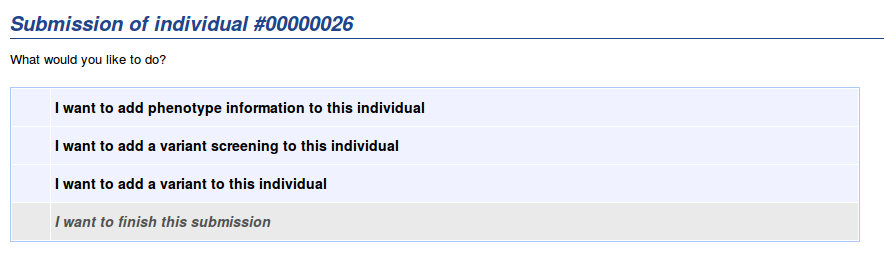
\includegraphics[width=\linewidth]{c08s01_screenshot_menu_add_information_to_individual.png}}%
  \caption{%
    After completing the data entry form, you can choose to add phenotype information
     (if a disease or ``healty/control'' has been selected) or a variant screening to this individual.
    A submission can only be finished after at least one screening with a variant is filled in.}
  \label{fig:submission_of_individual}
  \end{shaded}
\end{figure}



\clearpage
\hypertarget{ssec:add_phenotype_information_to_an_individual}{}
\subsection{Adding phenotype information to the individual}
\begin{wrapfigure}[3]{r}{8cm} % Only wrap for 3 lines
  \vspace{-25pt}
  \begin{leftbar}
    Required level: Submitter\\
    Available from: LOVD 3.0 Build 01
  \end{leftbar}
\end{wrapfigure}
When you created an individual, and this individual has been diagnosed with one or more diseases,
 or when this individual is marked as healthy/control, it is possible to add extra phenotype details to
 this individual.
Select ``I want to add phenotype information to this individual'' (figure
 \hyperlink{fig:submission_of_individual}{\ref{fig:submission_of_individual}}), fill all required fields and click
 ``Create phenotype information entry''.

The option ``I want to add phenotype information to this individual'' is disabled when no relation to
 diseases has been selected during the creation of this individual.
If you wish to add phenotype information while this option is disabled, you have to edit the individual, see
 section ``\hyperlink{ssec:add_phenotype}{\nameref{ssec:add_phenotype}}'' on how to proceed.



\hypertarget{ssec:add_variant_screening_to_an_individual}{}
\subsection{Adding a variant screening to the individual}
\label{ssec:add_variant_screening_to_an_individual}
\begin{wrapfigure}[3]{r}{8cm} % Only wrap for 3 lines
  \vspace{-25pt}
  \begin{leftbar}
    Required level: Submitter\\
    Available from: LOVD 3.0 Build 01
  \end{leftbar}
\end{wrapfigure}
By selecting ``I want to add a variant screening to this individual'' you can add a screening to the individual.
For ``Detection template'', ``Technique(s) used'' and ``Genes screened'', more than one item can be selected.
Complete the form, and when ready click ``Create screening information entry''.
When the entry is successful, a message is displayed for several seconds:
 ``Successfully created the screening entry!''.
Hereafter you are redirected to a menu where you can choose how to proceed:
\begin{figure}[ht]
  \begin{shaded}
  \frame{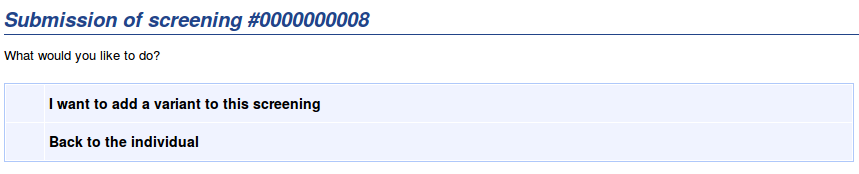
\includegraphics[width=\linewidth]{c08s01_screenshot_menu_add_variant_to_screening.png}}%
  \caption{%
    After adding a screening, you can add a variant to this screening.
    ``Back to the individual'' will leave this screening unfinished, and will return
     you to the choice to add phenotype information or another screening.}
  \end{shaded}
\end{figure}



\hypertarget{ssec:add_variant_to_a_screening}{}
\subsection{Adding a variant to a screening}
\label{ssec:add_variant_to_a_screening}
\begin{wrapfigure}[3]{r}{8cm} % Only wrap for 3 lines
  \vspace{-25pt}
  \begin{leftbar}
    Required level: Submitter\\
    Available from: LOVD 3.0 Build 01
  \end{leftbar}
\end{wrapfigure}
After adding a screening, you can add a variant to this screening.
It is possible to add more than one variant to a screening.
A submission can only be finished when at least one variant has been added to the submission.
\begin{figure}[ht]
  \begin{shaded}
  \frame{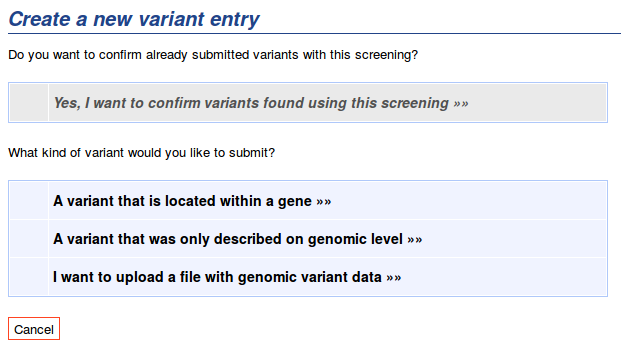
\includegraphics[width=\linewidth]{c08s01_screenshot_menu_create_new_variant_entry.png}}%
  \caption{%
    Creating a new variant entry.
    Note: Only managers and up have the option ``I want to upload a file with genomic variant data'' available.}
  \end{shaded}
\end{figure}

\subsubsection{Confirming variants using a screening}
When different variant screenings have been applied to the individual, for instance to confirm
 a variant found using a different method, the screenings can be stored separately in the database.
Multiple screenings can be linked to the same variant, or have their own sets of variants.
The option to confirm variants using a screening is only available when at least two
 screenings are added to the individual and variants have already been submitted.
After choosing this option, you are shown a list of variants already linked to other screenings
 of the individual, but not to the currently selected screening.
Click the checkmarks left of the variants that you would like to mark as confirmed, and click ``Save variant
 list''.
\begin{figure}[ht]
  \begin{shaded}
  \frame{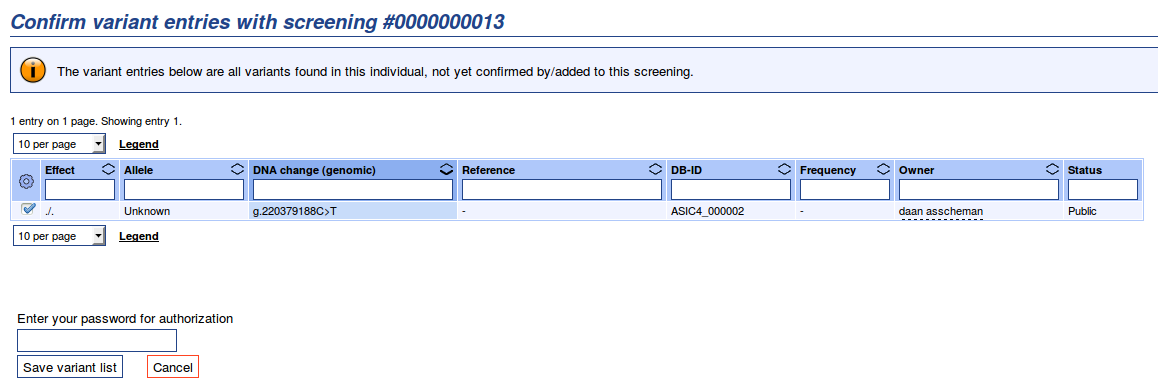
\includegraphics[width=\linewidth]{c08s01_screenshot_confirm_variant_using_screening.png}}%
  \caption{%
    Select a variant to confirm.
    Shown are the variants already linked to other screenings of the individual,
     but not to the currently selected screening.}
  \end{shaded}
\end{figure}

\subsubsection{Adding a variant located within a gene}
After choosing this option, you are shown a list of genes.
If certain genes have been selected while creating the screening, these are pre-selected.
You can remove or edit the pre-selection by removing or editing the configured filter in the ``Symbol'' column.
Then click the gene for which you want add a variant to proceed to the variant entry form.
You can check the help icon next to the form fields to see details
 about the fields and suggestions on how to use the fields.
Complete the form, and when ready, click the ``Create variant entry'' button.
If successful, you are redirected to the options to submit more variants, or return to the individual.
\begin{figure}[ht]
  \begin{shaded}
  \frame{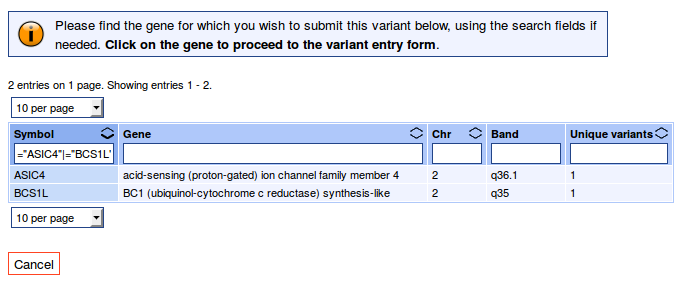
\includegraphics[width=\linewidth]{c08s01_screenshot_add_variant_located_within_gene.png}}%
  \caption{%
    Click the gene for which you want to submit a variant.}
  \end{shaded}
\end{figure}

\subsubsection{Adding a variant only described on genomic level}
You can create a variant which is only described on genomic level.
The data entry form is similar to the form for adding a variant within a gene, but lacks the transcript-specific fields.
Check the help icons next to the form fields to see details
 about the fields and suggestions on how to use the fields.
Complete the form, and when ready, click the ``Create variant entry'' button.
If successful, you are redirected to the options to submit more variants, or return to the individual.

\subsubsection{Uploading file with genomic variant data}
If you are a manager or higher, you can upload a file with genomic variant data.
This option is not displayed for users with levels lower than manager.
For uploading genomic variant data files two formats are supported:
 Variant Call Format (VCF) version 4.0 or higher and SeattleSeq Annotation files.
% STUB: Expand later, with screenhots and extensive explanation, perhaps not here but in a different place
% (own section in this chapter would seem good).



\hypertarget{ssec:add_variant_to_an_individual}{}
\subsection{Adding a variant to the individual}
\begin{wrapfigure}[3]{r}{8cm} % Only wrap for 3 lines
  \vspace{-25pt}
  \begin{leftbar}
    Required level: Submitter\\
    Available from: LOVD 3.0 Build 01
  \end{leftbar}
\end{wrapfigure}
The option ``Add a variant to this individual'' as displayed in figure \ref{fig:submission_of_individual} is only
 available when you already created a screening, and you selected ``Back to the individual'' after creating a
 screening.

When you want to add a variant to the individual, using a screening you previously created,
 you have to select the appropriate screening.
Click the ``Add a variant to this individual'' option, then click the screening you wish to add another variant to,
 and you will be redirected to the menu where you can submit a new variant.
See section ``\hyperlink{ssec:add_variant_to_a_screening}{\nameref{ssec:add_variant_to_a_screening}}''.
\clearpage



\hypertarget{ssec:finish_submission}{}
\subsection{Finishing the submission}
\begin{wrapfigure}[3]{r}{8cm} % Only wrap for 3 lines
  \vspace{-25pt}
  \begin{leftbar}
    Required level: Submitter\\
    Available from: LOVD 3.0 Build 01
  \end{leftbar}
\end{wrapfigure}
The option ``I want to finish this submission'' is enabled for submitters when they completed a submission,
 i.e., an individual, screening and at least one variant have been added.
Finishing a submission will send an email to the curator(s) of the gene(s) affected by the variant(s) submitted,
 or the manager(s), for variants described only on genomic level.
They are thereby requested to publish the newly submitted data.
You as submitter of the data, will receive a copy of this email.
As long as the data is not yet published, the data is invisible for other users.
You will however be able to see the data previously submitted by you, at all times.





\hypertarget{sec:interrupted_submission}{}
\section{Continuing an unfinished submission}
\begin{wrapfigure}[3]{r}{8cm} % Only wrap for 3 lines
  \vspace{-25pt}
  \begin{leftbar}
    Required level: Submitter\\
    Available from: LOVD 3.0 Build 01
  \end{leftbar}
\end{wrapfigure}
If, for whatever reason, a data submission has not been finished, it is stored in the list of unfinished submissions.
This also means that the curator(s) did not get an email with the request to publish the newly submitted data.
You can continue an unfinished submission at any time, adding any missing information,
 and finishing the submission to alert the curator(s) of the new data.
To proceed with an unfinished submission, select ``Unfinished submissions'' in the top right corner of the screen.
You will see an overview of data submissions which are not yet finished.
Select any submission to proceed.
The normal submission process will continue where it was left, for instructions
 see the appropriate section in this chapter.





\hypertarget{sec:submit_summary_variant_data}{}
\section{Submitting summary variant data}
\label{submit_summary_variant_data}
\begin{wrapfigure}[3]{r}{8cm} % Only wrap for 3 lines
  \vspace{-25pt}
  \begin{leftbar}
    Required level: Curator\\
    Available from: LOVD 3.0 Build 01
  \end{leftbar}
\end{wrapfigure}
If you are a curator or higher, you can choose to submit only summary variant data.
This means that no individual, phenotype or screening data is submitted, only variant data.
Although you can submit summary variant data, it is highly discouraged because individual and phenotype
 data make the variant data much more valuable.
An example of a valid reason to submit summary variant data is for storing variant frequency data of large populations.





\hypertarget{sec:add_data_finished_submissions}{}
\section{Adding data to already finished submissions}
\begin{wrapfigure}[3]{r}{8cm} % Only wrap for 3 lines
  \vspace{-25pt}
  \begin{leftbar}
    Required level: Submitter\\
    Available from: LOVD 3.0 Build 01
  \end{leftbar}
\end{wrapfigure}
It is still possible for the submitter to add data to an individual or a screening when a submitter finished
 the submission, regardless of whether the curator published the data or not.



\hypertarget{ssec:add_variant}{}
\subsection{Adding a variant to a screening}
\begin{wrapfigure}[4]{r}{5cm} % Only wrap for 4 lines
  \vspace{-25pt}
  \begin{framed}
    \raisebox{-0.5mm}{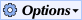
\includegraphics[width=2.1cm]{options_button.png}}\\Options menu button
  \end{framed}
\end{wrapfigure}
To add a variant to an existing screening, click on the ``Screenings'' tab and select
 a screening for which you are authorized.
Click on the ``Options'' menu button to open up the screening entry's menu.
If you do not see the ``Options'' menu button, you are not logged in or you do not have rights to edit this
 screening.
In the opened menu, click ``Add variant to screening''.
From here you can follow the steps described in the section
 ``\hyperlink{ssec:add_variant_to_a_screening}{\nameref{ssec:add_variant_to_a_screening}}''.
After you submitted the variant data, LOVD sends an email to the curator(s) and redirects you to the variant
 overview.



\hypertarget{ssec:add_screening}{}
\subsection{Adding screening to individual}
\begin{wrapfigure}[4]{r}{5cm} % Only wrap for 4 lines
  \vspace{-25pt}
  \begin{framed}
    \raisebox{-0.5mm}{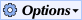
\includegraphics[width=2.1cm]{options_button.png}}\\Options menu button
  \end{framed}
\end{wrapfigure}
To add a screening to an existing individual, click on the ``Indivi\-duals'' tab and select an individual for
 which you are authorized.
Click on the ``Options'' menu button to open up the individual entry's menu.
If you do not see the ``Options'' menu button, you are not logged in or you do not have rights to edit this
 individual.
In the opened menu, click ``Add screening to individual'' to open up the screening data entry form.
You are now in the submission process described in section
 ``\hyperlink{ssec:add_variant_screening_to_an_individual}{\nameref{ssec:add_variant_screening_to_an_individual}}''.
The option ``Back to individual'' is not available when you submit a screening to an existing  individual.
You can only finish this submission, if you also add at least one new variant to this new screening,
 or select at least one previously submitted variant as confirmed by this new screening.
After finishing the submission, LOVD sends an email to the curator(s) requesting the publication of the submission.



\hypertarget{ssec:add_phenotype}{}
\subsection{Adding phenotype information to an individual}
\label{ssec:add_phenotype}
\begin{wrapfigure}[4]{r}{5cm} % Only wrap for 4 lines
  \vspace{-25pt}
  \begin{framed}
    \raisebox{-0.5mm}{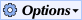
\includegraphics[width=2.1cm]{options_button.png}}\\Options menu button
  \end{framed}
\end{wrapfigure}
To add phenotype information to an existing individual, click on the ``Individuals'' tab and select an individual for
 which you are authorized.
Click on the ``Options'' menu button to open up the individual entry's menu.
If you do not see the ``Options'' menu button, you are not logged in or you do not have rights to edit this
 individual.
In the opened menu, click ``Add phenotype information to individual'' to open up the phenotype data entry form,
 or, in the case this individual has been diagnosed with multiple diseases,
 to select which disease you wish to add phenotype data for.
If you do not see the ``Add phenotype information to individual'' option,
 then the individual does not have any diseases linked yet.
In that case, edit the individual and select at least one disease from the list.

After you submitted the phenotype data, LOVD sends an email
 to the curator(s) and redirects you to the phenotype data overview.










\hypertarget{chap:download_n_import}{}
\chapter{Downloading \& importing data}
\hypertarget{sec:download_import_format}{}
\section{The LOVD3 import format}
\label{sec:download_import_format}
The LOVD3 import format is based on the LOVD2 tab-delimited import format,
 but all data is split into separate sections, preventing data duplication.
Examples of sections are Genes, Transcripts, and Diseases.
Each section has its own set of fields.
Sections refer to each other using IDs.
For instance, the Transcripts section has a \emph{geneid} field that refers
 to an entry in the Genes section with the same value in its \emph{id} field.
This way, transcripts are connected to genes.

\begin{figure}[ht]
  \begin{shaded}
    \scriptsize
    \begin{verbatim}
### LOVD-version 3000-010 ### Full data download ### To import, do not remove or alter this header ###
# charset = UTF-8

## Genes ## Do not remove or alter this header ##
"{{id}}"	"{{name}}"	"{{chromosome}}"	"{{chrom_band}}"	"{{id_hgnc}}"	"{{id_entrez}}"	"{{id_omim}}"
"IVD"	"isovaleryl-CoA dehydrogenase"	"15"	"q14-q15"	"6186"	"3712"	"607036"

## Transcripts ## Do not remove or alter this header ##
"{{id}}"	"{{geneid}}"	"{{name}}"	"{{id_ncbi}}"	"{{id_protein_ncbi}}"
"00064"	"IVD"	"isovaleryl-CoA dehydrogenase, transcript variant 1"	"NM_002225.3"	"NP_002216.2"

## Diseases ## Do not remove or alter this header ##
"{{id}}"	"{{symbol}}"	"{{name}}"	"{{id_omim}}"
"00006"	"IVA"	"isovaleric acidemia"	"243500"

## Genes_To_Diseases ## Do not remove or alter this header ##
"{{geneid}}"	"{{diseaseid}}"
"IVD"	"00006"

## Individuals ## Do not remove or alter this header ##
"{{id}}"	"{{owned_by}}"	"{{statusid}}"	"{{Individual/Lab_ID}}"	"{{Individual/Reference}}"
"00000124"	"00001"	"9"	"FB102"	"{PMID:Vockley et al (2000):10677295}"

## Individuals_To_Diseases ## Do not remove or alter this header ##
"{{individualid}}"	"{{diseaseid}}"
"00000124"	"00006"

## Screenings ## Do not remove or alter this header ##
"{{id}}"	"{{individualid}}"	"{{owned_by}}"	"{{Screening/Technique}}"	"{{Screening/Template}}"
"0000000116"	"00000124"	"00001"	"RT-PCR;SEQ"	"DNA;RNA"

## Screenings_To_Genes ## Do not remove or alter this header ##
"{{screeningid}}"	"{{geneid}}"
"0000000116"	"IVD"
    \end{verbatim}
  \caption{%
    Example (partial) LOVD import format file.
    This example file contains information about the IVD gene, its first transcript variant,
     the IVA disease, the link between the IVD gene and the IVA disease, and an individual linked
     to the IVA disease and screened for variants in the IVD gene.
    Note the \emph{geneid} field in the Transcripts section, which links a transcript to a gene,
     and the \emph{individualid} field in the Screenings section, which links a screening to an individual.
    The link between genes and diseases and between screenings and genes are in a separate section because
     each gene can be linked to multiple diseases, and each screening can test for variants in multiple genes.
    Please note that a full LOVD download contains many more sections, and more columns.
    This file has been shortened to fit this page.
    \emph{This example file is therefore not a valid import file.}}
  \end{shaded}
\end{figure}

The first line of the file contains the file's header line,
 which indicates the LOVD version number as well as the type of file.
The LOVD version number is encoded and provided by LOVD when creating a download.
When importing, LOVD can decode the version and in case the download format has changed between versions,
 convert the data into the correct format.
When this line is not included in the file that is imported, LOVD cannot process the file, and halt.

The file's data sections are indicated by lines starting with two hash characters (\#\#),
 followed by the name, again two hash characters, and a note that the header should not be modified or removed.
Other lines starting with two hash characters are regarded comments.
A downloaded file may contain comments, like the number of entries for each section.
\vskip \baselineskip

\noindent
The following sections are currently recognized:
\begin{description}
  \item[Columns] \hfill \\
    Custom columns and their system-wide settings.
    In a full data download, this section contains records created during
     installation of LOVD as well as records created by users.
    During import, columns in the import file that already exist in the database are skipped.
    In that case a warning is displayed, but the import will continue.
  \item[Genes] \hfill \\
    Genes, including external IDs. \emph{Can currently not yet be imported.}
    When importing, genes can be listed in the file, but they should already be present in the database.
    If not present, they should be created manually before importing the file.
    Links between genes and diseases are described in the ``Genes\_To\_Diseases'' section.
  \item[Transcripts] \hfill \\
    Transcript variants, including external IDs. \emph{Can currently not yet be imported.}
    When importing, transcripts can be listed in the file, but they should already be present in the database.
    If not present, they should be created manually before importing the file.
    A transcript entry is linked to a gene using the ``geneid'' field.
  \item[Diseases] \hfill \\
    General disease information.
    Diseases should have a unique name and OMIM ID.
    During import, diseases in the import file that already exist in the database
     (based on name or OMIM ID) are skipped.
    In that case a warning is displayed, but the import will continue.
    Links between diseases and genes are described in the ``Genes\_To\_Diseases'' section.
  \item[Genes\_To\_Diseases] \hfill \\
    Links genes and diseases by referring to their IDs.
  \item[Individuals]* \hfill \\
    Individuals and related information, like links to the parents of the individual.
    Links between individuals and diseases are described in the ``Individuals\_To\_Diseases'' section.
  \item[Individuals\_To\_Diseases] \hfill \\
    Links individuals to diseases.
  \item[Phenotypes]* \hfill \\
    Phenotype information of a certain individual, related to a certain disease.
    A phenotype entry is linked to a disease using the ``diseaseid'' field.
    A phenotype entry is linked to an individual using the ``individualid'' field.
  \item[Screenings]* \hfill \\
    Variant screening information, with which variants are detected.
    A screening is linked to an individual using the ``individualid'' field.
    Links between screenings and genes are described in the ``Screenings\_To\_Genes'' section.
    Links between screenings and variants are described in the ``Screenings\_To\_Variants'' section.
  \item[Screenings\_To\_Genes] \hfill \\
    Linking screenings to genes, indicating which genes were screened using a certain screening.
  \item[Variants\_On\_Genome]* \hfill \\
    Genomic information of all variants detected.
    Links between variants and screenings are described in the ``Screenings\_To\_Variants'' section.
  \item[Variants\_On\_Transcripts]* \hfill \\
    Possible effects on a transcript caused by a genomic variant.
    A variant on transcript is linked to a variant on genome using the ``id'' field.
  \item[Screenings\_To\_Variants] \hfill \\
    Linking screenings to variants, indicating which variants were detected using a certain screening.
\end{description}
\noindent
Categories indicated with an asterisk (*) are data types with custom columns
 (also see ``\hyperlink{sec:custom_column_categories}{\nameref{sec:custom_column_categories}}''),
 and the exact list of fields in this category depend on the LOVD settings.

Lines in the import file starting with one hash character are settings.
The following settings are currently recognized:
\begin{description}
  \item[charset] \hfill \\
    Indicates which carset was used when creating the file.
    During import, usually the file encoding is detected given the file's contents,
     in which case this setting is ignored.
\end{description}

Each section header is followed immediately by a line that indicates the names of the fields used in this section.
When reading a downloaded file, this nicely indicates which column represents which data.
When importing a file, being able to change this line allows you to skip certain columns
 or decide yourself in which order you would like to display the columns in the file.
To clearly separate the line with column names from the data lines,
 the column names are surrounded by two curly braces on each side (\{\{ and \}\}).
Field names can not contain spaces, match the field's name in the database exactly,
 and the field names are separated by exactly one tab character from each other.
\vskip \baselineskip

The section's data is also in tab-delimited format.
Each field is preferably enclosed by double quotes.
All existing quotes in the data, are escaped by the backslash character (\textbackslash),
 so \texttt{\symbol{34}} becomes \texttt{\textbackslash\symbol{34}}.
Other special characters are \texttt{\textbackslash{}t} for a tab character,
 and \texttt{\textbackslash{}r\textbackslash{}n} for a linebreak.



\subsection{Specific fields explained}
For each section, the import format contains all fields that are stored in the database.
Some of these fields are not displayed on the normal LOVD data entry forms, and therefore may cause confusion.
Others are displayed, but for the user appear as selection lists with human-readable values,
 whereas in the database only numbers are stored.
To aid in understanding these fields and their values, all fields that may cause confusion are listed here.

Custom columns are not listed here, since every LOVD installation has different
 columns enabled and custom columns provide explanations about their use by themselves.

\begin{description}
  \item[allele] (from section Variants\_On\_Genome)\hfill \\
  Indicates on which allele the variant is located.
  Does not necessarily imply inheritance!\\
  \begin{tabular}{>{\bfseries}p{0.6cm} p{4.0cm} p{10.0cm}}
    ID & \textbf{Name} & \textbf{Description}\\ \hline \hline
    0 & Unknown & Heterozygous, parents not screened, or de novo and allele couldn't be confirmed\\ \hline
    1 & Parent \#1 & Heterozygous, parents not screened, but useful in combination with `Parent \#2` to indicate cis or
      trans compound heterozygosity\\ \hline
    2 & Parent \#2 & Heterozygous, parents not screened, but useful in combination with `Parent \#1` to indicate cis or
      trans compound heterozygosity\\ \hline
    3 & Both (homozygous) & Variant is present on both alleles\\ \hline
    10 & Paternal (inferred) & Variant is on paternal allele, not confirmed in father but inferred from other
      information\\ \hline
    11 & Paternal (confirmed) & Variant is on paternal allele, confirmed in father\\ \hline
    20 & Maternal (inferred) & Variant is on maternal allele, not confirmed in mother but inferred from other
      information\\ \hline
    21 & Maternal (confirmed) & Variant is on maternal allele, confirmed in mother\\ \hline
  \end{tabular}
%  \item[allow\_count\_all] (from section Columns)\hfill \\
  \item[chromosome] (from sections Genes and Variants\_On\_Genome)\hfill \\
  The chromosome related to this entry (gene or variant).
  When importing, do not fill `chr' here as prefix, just the chromosome number or letter.
  \item[chrom\_band] (from section Genes)\hfill \\
  The chomosome band, like `q15'.
  \item[col\_order] (from section Columns)\hfill \\
  The order in which the columns of this column's category are shown.
  Low values are shown before higher values.
  \item[created\_by] (from sections Columns, Genes, Transcripts, Diseases, Individuals, Phenotypes,
   Screenings and Variants\_On\_Genome)\hfill \\
  The internal ID of the user that created this data entry.
  If left empty during import, the current user performing the import will be selected
   as the creator of this data entry.
  Creators are allowed to edit the entry and add new data to the entry.
  They are fixed, and can not be re-assigned at a later time.
  \item[created\_date] (from sections Columns, Genes, Transcripts, Diseases, Individuals, Phenotypes,
   Screenings and Variants\_On\_Genome)\hfill \\
  The date the entry was created, in the format YYYY-MM-DD HH:MM:SS.
  \item[description\_form] (from section Columns)\hfill \\
  The column's notes on the data entry form.
  This text is shown on the data entry form, just below the data field, for instance as clarification.
  See also section ``\hyperlink{sec:custom_column_create}{\nameref{sec:custom_column_create}}''.
  \item[description\_legend\_short] (from section Columns)\hfill \\
  Description on short legend for this custom column.
  See also section ``\hyperlink{sec:custom_column_create}{\nameref{sec:custom_column_create}}''.
  \item[description\_legend\_full] (from section Columns)\hfill \\
  Description on full legend for this custom column.
  See also section ``\hyperlink{sec:custom_column_create}{\nameref{sec:custom_column_create}}''.
  \item[effectid] (from sections Variants\_On\_Genome and Variants\_On\_Transcripts)\hfill \\
  The variant's affect on a protein's function.
  The first digit indicates the reported variant's effect.
  The second digit indicates the variant's effect as concluded by the curator.
  The possible values of each digit:\\
  \begin{tabular}{>{\bfseries}p{0.6cm} p{2.3cm} p{11.7cm}}
    ID & \textbf{Name} & \textbf{Description}\\ \hline \hline
    1 & - & Does not affect function, strong proof\\ \hline
    3 & -? & Probably does not affect function, strong evidence\\ \hline
    5 & ? & Effect unknown\\ \hline
    7 & +? & Probably affects function, strong evidence\\ \hline
    9 & + & Affects function, strong proof\\ \hline
  \end{tabular}

  A score of 97 means a variant is reported to effect the function of the protein having strong proof, but the curator
   thinks more proof is needed, still accepting there is strong evidence for the variant's effect.
  All options are:
  \vskip \baselineskip

  \begin{minipage}[t]{3.15cm}
    \begin{tabular}{>{\bfseries}p{0.6cm} p{1.4cm}}
      ID & \textbf{Name}\\ \hline \hline
      11 & -/-\\ \hline
      13 & -/-?\\ \hline
      15 & -/?\\ \hline
      17 & -/+?\\ \hline
      19 & -/+\\ \hline
    \end{tabular}
  \end{minipage}
  \begin{minipage}[t]{3.15cm}
    \begin{tabular}{>{\bfseries}p{0.6cm} p{1.4cm}}
      ID & \textbf{Name}\\ \hline \hline
      31 & -?/-\\ \hline
      33 & -?/-?\\ \hline
      35 & -?/?\\ \hline
      37 & -?/+?\\ \hline
      39 & -?/+\\ \hline
    \end{tabular}
  \end{minipage}
  \begin{minipage}[t]{3.15cm}
    \begin{tabular}{>{\bfseries}p{0.6cm} p{1.4cm}}
      ID & \textbf{Name}\\ \hline \hline
      51 & ?/-\\ \hline
      53 & ?/-?\\ \hline
      55 & ?/?\\ \hline
      57 & ?/+?\\ \hline
      59 & ?/+\\ \hline
    \end{tabular}
  \end{minipage}
  \begin{minipage}[t]{3.15cm}
    \begin{tabular}{>{\bfseries}p{0.6cm} p{1.4cm}}
      ID & \textbf{Name}\\ \hline \hline
      71 & +?/-\\ \hline
      73 & +?/-?\\ \hline
      75 & +?/?\\ \hline
      77 & +?/+?\\ \hline
      79 & +?/+\\ \hline
    \end{tabular}
  \end{minipage}
  \begin{tabular}{>{\bfseries}p{0.6cm} p{1.4cm}}
    ID & \textbf{Name}\\ \hline \hline
    91 & +/-\\ \hline
    93 & +/-?\\ \hline
    95 & +/?\\ \hline
    97 & +/+?\\ \hline
    99 & +/+\\ \hline
  \end{tabular}
  \item[fatherid] (from section Individuals)\hfill \\
  Optional; The internal ID of the individual in the database that is the father of this individual.
  \item[form\_type] (from section Columns)\hfill \\
  The custom column's form type definition.
  When importing new custom columns, we recommend you use the Data type wizard available
   when creating a new custom column, and to use the form type definition generated by the wizard.
  See also section ``\hyperlink{sec:custom_column_create}{\nameref{sec:custom_column_create}}''.
  \item[head\_column] (from section Columns)\hfill \\
  The custom column's header, shown above the column in data views.
  See also section ``\hyperlink{sec:custom_column_create}{\nameref{sec:custom_column_create}}''.
  \item[hgvs] (from section Columns)\hfill \\
  If set to 1, this column is HGVS recommended.
  These columns can not be removed.
  This setting can not be set when importing columns.
  Default value is 0.
%  \item[id\_mutalyzer] (from section Transcripts)\hfill \\
  \item[imprinting] (from section Genes)\hfill \\
  Whether or not a gene is imprinted (either maternal or paternal).
  \item[mandatory] (from section Columns)\hfill \\
  If set to 1, this column is mandatory.
  When entering new data, this custom column's field must be filled in.
  See also section ``\hyperlink{sec:custom_column_create}{\nameref{sec:custom_column_create}}''.
  Default value is 0.
  \item[mapping\_flags] (from section Variants\_On\_Genome)\hfill \\
  Information about how LOVD handles the mapping of this variant.
  LOVD has an automatic mapping script that finds transcripts in the range of a genomic variant, and can annotate the
    genomic variant on the transcript using the Mutalyzer web service.
  Whether or not LOVD is allowed to map the variant, and how LOVD will handle the mapping, is stored in this field.
  This field is a boolean flag column; multiple options can be grouped in this field by adding the numbers up.
  Possible values:\\
  \begin{tabular}{>{\bfseries}p{0.6cm} p{7.7cm} p{6.3cm}}
    ID & \textbf{Name} & \textbf{Description}\\ \hline \hline
    1 & MAPPING\_ALLOW & When set, the variant can be map\-ped by the LOVD mapping script\\ \hline
    2 & MAPPING\_ALLOW\_CREATE\_GENES & When set, LOVD is allowed to create new genes in the database if needed to
      annotate the variant\\ \hline
    4 & MAPPING\_IN\_PROGRESS & \emph{Not used when importing}; when set, LOVD is currently busy mapping the
      variant\\ \hline
    8 & MAPPING\_NOT\_RECOGNIZED & \emph{Not used when importing}; when set, LOVD did not recognize the variant, and
      was therefore unable to map the variant\\ \hline
    16 & MAPPING\_ERROR & \emph{Not used when importing}; when set, LOVD has encountered an error while mapping\\ \hline
    32 & MAPPING\_DONE & \emph{Not used when importing}; when set, LOVD is done mapping the variant, regardless of
      whether the variant actually got mapped\\ \hline
  \end{tabular}

  For instance, a value of 11 means for this variant mapping has been enabled (1), LOVD is allowed to create new genes
    while mapping the variant (2), but LOVD does not recognize the variant and therefore can not map it (8). 1 + 2 + 8
    = 11.
  \item[motherid] (from section Individuals)\hfill \\
  Optional; The internal ID of the individual in the database that is the mother of this individual.
  \item[mysql\_type] (from section Columns)\hfill \\
  The custom column's MySQL data type.
  When importing new custom columns, we recommend you use the Data type wizard available
   when creating a new custom column, and to use the MySQL data type generated by the wizard.
  See also section ``\hyperlink{sec:custom_column_create}{\nameref{sec:custom_column_create}}''.
  \item[note\_index] (from section Genes)\hfill \\
  Notes that should appear on the gene home page.
  \item[note\_listing] (from section Genes)\hfill \\
  Notes that should appear on gene-specific data listings.
  \item[owned\_by] (from section Individuals, Phenotypes, Screenings and Variants\_On\_Genome)\hfill \\
  Optional; The internal ID of the user that owns this data entry.
  Owners are allowed to edit the entry and add new data to the entry.
  Owners are not fixed, and can be re-assigned.
  When no value is provided during import, this value is set to the user ID of the user importing the data.
  \item[panelid] (from section Individuals)\hfill \\
  Optional; The internal ID of the individual in the database that represents the group
   to which this individual or group of individuals belong to.
  \item[panel\_size] (from section Individuals)\hfill \\
  The number of individuals represented by this entry (default: 1).
  Only used when multiple individuals, for instance from one family, are aggregated into one entry in the database.
  \item[position\_c\_cds\_end] (from section Transcripts)\hfill \\
  The position, relative to the translation start site, of where the translation ends.
  Is always a positive whole number, should always be dividable by three.
  \item[position\_c\_mrna\_start] (from section Transcripts)\hfill \\
  The position, relative to the translation start site, of where the transcript starts.
  Is always a negative whole number.
  \item[position\_c\_mrna\_end] (from section Transcripts)\hfill \\
  The position, relative to the translation start site, of where the transcript ends.
  Is always a positive whole number.
  \item[position\_c\_start] (from section Variants\_On\_Transcripts)\hfill \\
  The position, relative to the translation start site, of the first base of the variant.
  The first base of the variant is defined by the HGVS nomenclature rules, and may be the same as the last base.
  \item[position\_c\_start\_intron] (from section Variants\_On\_Transcripts)\hfill \\
  The position, relative to the start or end (whichever is closest) of the intron, of the first base of the variant.
  The first base of the variant is defined by the HGVS nomenclature rules, and may be the same as the last base.
  This field only applies to variants that start or end in an intron.
  \item[position\_c\_end] (from section Variants\_On\_Transcripts)\hfill \\
  The position, relative to the translation start site, of the last base of the variant.
  The last base of the variant is defined by the HGVS nomenclature rules, and may be the same as the first base.
  \item[position\_c\_end\_intron] (from section Variants\_On\_Transcripts)\hfill \\
  The position, relative to the start or end (whichever is closest) of the intron, of the last base of the variant.
  The last base of the variant is defined by the HGVS nomenclature rules, and may be the same as the first base.
  This field only applies to variants that start or end in an intron.
  \item[position\_g\_mrna\_start] (from section Transcripts)\hfill \\
  The genomic position, relative to the chromosome, of where the transcript starts.
  \item[position\_g\_mrna\_end] (from section Transcripts)\hfill \\
  The genomic position, relative to the chromosome, of where the transcript ends.
  \item[position\_g\_start] (from section Variants\_On\_Genome)\hfill \\
  The genomic position, relative to the chromosome, of the first base of the variant.
  The first base of the variant is defined by the HGVS nomenclature rules, and may be the same as the last base.
  \item[position\_g\_end] (from section Variants\_On\_Genome)\hfill \\
  The genomic position, relative to the chromosome, of the last base of the variant.
  The last base of the variant is defined by the HGVS nomenclature rules, and may be the same as the first base.
  \item[preg\_pattern] (from section Columns)\hfill \\
  For text field custom columns, regular expression checks can be performed.
  See also section ``\hyperlink{sec:custom_column_create}{\nameref{sec:custom_column_create}}''.
  \item[public\_view] (from section Columns)\hfill \\
  If set to 1, this column's contents are visible to the public (only for public entries).
  See also section ``\hyperlink{sec:custom_column_create}{\nameref{sec:custom_column_create}}''.
  \item[public\_add] (from section Columns)\hfill \\
  If set to 1, submitters can fill in this field.
  Otherwise, only curators and higher level users can enter data in this field.
  \item[refseq\_UD] (from section Genes)\hfill \\
  This is an internal ID for the genomic reference sequence, generated by Mutalyzer.
  \item[select\_options] (from section Columns)\hfill \\
  When the custom column is a selection field, the selection options are listed here.
  See also section ``\hyperlink{sec:custom_column_create}{\nameref{sec:custom_column_create}}'' for the format.
  Please remember that linebreaks in the LOVD import format are displayed
   as \texttt{\textbackslash{}r\textbackslash{}n}.
  \item[standard] (from section Columns)\hfill \\
  If set to 1, this column is enabled by default.
  When importing, this is only useful for shared custom columns.
  When set, the column will then be enabled by default for a new disease or gene, depending on the column category.
  See also section ``\hyperlink{sec:custom_column_create}{\nameref{sec:custom_column_create}}''.
  Default value is 0.
  \hypertarget{ssec:column_statusid}{}
  \item[statusid] (from section Individuals, Phenotypes and Variants\_On\_Genome)\hfill \\
  Optional; This numeric status ID defines if the data is public or not.\\
  \begin{tabular}{>{\bfseries}p{0.6cm} p{2.3cm} p{11.7cm}}
    ID & \textbf{Name} & \textbf{Description}\\ \hline \hline
    1 & In progress & \emph{Not used when importing}; data entry is in the process of being submitted\\ \hline
    2 & Pending & \emph{Not used when importing}; data entry has been submitted, awaiting approval of curator\\ \hline
    4 & Non public & Data entry is not public, hidden from view for non-authorized users\\ \hline
    7 & Marked & Data entry is public but marked, shows up as red for authorized users\\ \hline
    9 & Public & Data entry is public\\ \hline
  \end{tabular}
  \vskip \baselineskip
  Data with status ``In progress'' or ``Pending'', respectively value 1 and 2, can not be imported.
  Instead, there are 3 options:
  \begin{enumerate}
    \item If the import file originates from a different LOVD installation,
       then curate the data there, and download the file again.
    \item Change the statusid value to a valid value, being 4 or higher.
    \item Exclude this record for import, by either removing it from the import file,
       or hiding the record by putting a \# in the beginning of the line.
      If you do this, make sure that all related data from other sections are excluded as well,
       or LOVD will return errors when trying to resolve references in the file.
  \end{enumerate}

  When no value is provided during import, this value is set to `9' (Public).
  \item[symbol] (from section Diseases) \hfill \\
  The disease's abbreviation, preferably the most commonly used one.
  \item[type] (from section Variants\_On\_Genome)\hfill \\
  The type of variant on DNA level, as defined by the Mutalyzer web service.
  All possible values are:\\
  \begin{tabular}{>{\bfseries}p{2.2cm} p{3.4cm} p{9cm}}
    ID & \textbf{Name} & \textbf{Description}\\ \hline \hline
    compound & Compound variant & \emph{Not normally in use}; multiple variants grouped together\\ \hline
    del & Deletion & One or more DNA bases have been deleted\\ \hline
    delins & Deletion/Insertion & One or more DNA bases have been deleted, while others have been inserted; when not a
      substitution\\ \hline
    dup & Duplication & Duplication of one or more DNA bases\\ \hline
    ins & Insertion & Insertion of one or more DNA bases; when not a duplication\\ \hline
    subst & Substitution & One DNA base has been replaced by another\\ \hline
  \end{tabular}
  \item[variants\_found] (from section Screenings)\hfill \\
  If set to 1, this screening is reported to have found variants.
  If set to 0, this screening is reported to not have found variants.
  Please note that other values are not allowed.
  \item[width] (from section Columns)\hfill \\
  The displayed column width in pixels.
  See also section ``\hyperlink{sec:custom_column_create}{\nameref{sec:custom_column_create}}''.
%  \item[] (from section Genes)\hfill \\
%"{{refseq}}"	"{{refseq\_url}}"	"{{disclaimer}}"	"{{disclaimer\_text}}"	"{{header}}"	"{{header\_align}}"	"{{footer}}"	"{{footer\_align}}"	"{{updated\_by}}"	"{{updated\_date}}"
\end{description}





\hypertarget{sec:download_import_data}{}
\section{Downloading \& importing data}
\hypertarget{ssec:download_data}{}
\subsection{Downloading data from LOVD}
\begin{wrapfigure}[3]{r}{8cm} % Only wrap for 3 lines
  \vspace{-25pt}
  \begin{leftbar}
    Required level: Submitter\\
    Available from: LOVD 3.0 Build 01
  \end{leftbar}
\end{wrapfigure}
For backup purposes or to move data sets from one LOVD into another, LOVD supports different download options.
All downloaded file types lack the LOVD system settings, registered user accounts, and object-specific custom
 column settings.

In order to have a full backup, for instance to restore LOVD in case of a hardware failure, more information
 is needed.
It is therefore recommended not to rely only on this feature for a full backup of LOVD.
However, it works perfectly as a backup for your variant and patient data, for instance if you accidentally
 deleted the wrong entry or the wrong column.

If you're planning large parallel changes to data entries in LOVD using spreadsheet software such as
 OpenOffice.org Calc or MS Excel, you could use the download files as a starting point.
In that case, read the instructions at ``\hyperlink{sec:download_import_full_data}
 {\nameref{sec:download_import_full_data}}'' before you begin.

% Subsection here about the downloading of all overviews. Quick download, not usable for import.
\begin{comment}
In case you provided search terms, only the results will be included in the download file.
Also the order in the downloaded file is equal to the order of the entries on the screen.
\end{comment}



\hypertarget{ssec:importing_data}{}
\subsection{Importing data sets into LOVD}
\begin{wrapfigure}[3]{r}{8cm} % Only wrap for 3 lines
  \vspace{-25pt}
  \begin{leftbar}
    Required level: Curator\\
    Available from: LOVD 3.0 Build 01
  \end{leftbar}
\end{wrapfigure}
For managers it is possible to import data directly into LOVD, using the LOVD3 import format.
For curators, only simulation is available (see below), starting from LOVD 3.0-14.
See section ``\hyperlink{sec:download_import_format}{\nameref{sec:download_import_format}}'' for more details about the
 file format.
Files created or modified using spreadsheet software such as OpenOffice.org Calc or MS Excel must be saved as
 a text file.
The file must be tab delimited, otherwise LOVD will produce an error.

To import a dataset to LOVD, click the ``Import data'' link from the ``Setup'' tab dropdown menu,
 or from the setup area, click the ``Import data using the LOVD import format'' link listed under
 ``Download \& Import''.
Curators can import data from the Configuration area. 
Click the ``Import data using the LOVD import format'' link listed under ``Download \& Import''.

The LOVD import has a simulate option, allowing you to check if the import file is correct, without importing anything.
Check the ``Simulate (don't actually import the data)'' checkbox to use this simulation option.
This option is always enabled for curators, and cannot be disabled.
This allows curators to test their import files,
 but it still requires a manager or up to actually import the file.

The import mode is an option which will be extended in the near future.
For now only ``Add only, treat all data a new'' is available.
This means all importable data in the import file, is inserted as new in the database,
 also if the identifiers used are already present in the database.
In the future, the option ``Update existing data \& add new data''
 will allow updating data in the database by importing a file.



 

\hypertarget{sec:download_import_full_data}{}
\section{Downloading \& importing the complete data}
\label{sec:download_import_full_data}



\hypertarget{ssec:download_full_data}{}
\subsection{Downloading the complete data set from LOVD}
\begin{wrapfigure}[3]{r}{8cm} % Only wrap for 3 lines
  \vspace{-25pt}
  \begin{leftbar}
    Required level: Manager\\
    Available from: LOVD 3.0 Build 01
  \end{leftbar}
\end{wrapfigure}
LOVD supports a full download that contains most (currently not all) data stored in LOVD.
The data sections included in the download file are:
 Columns, Genes, Transcripts, Diseases, Genes\_To\_Diseases, Individuals, Individuals\_To\_Diseases,
 Phenotypes, Screenings, Screenings\_To\_Genes, Variants\_On\_Genome, Variants\_On\_Transcripts
 and Screenings\_To\_Variants.
In order to have a full backup, for instance to restore LOVD in case of a hardware failure,
 more information is needed.
The download file lacks the LOVD system settings, registered user accounts, and object-specific custom column settings.
It is therefore recommended not to rely only on this feature for a full backup of LOVD.
However, it works perfectly as a backup for your variant and patient data, for instance if you accidentally
 deleted the wrong entry or the wrong column.

To download the full dataset from LOVD, click the ``Download all data'' link from the ``Setup'' tab dropdown
 menu, or from the setup area, click the ``Download all data in LOVD import format'' link listed under
 ``Download \& Import''.
The download begins immediately.
Depending on your browser, it will save the file to a default location on your hard disk,
 or ask you whether to open or to save the file.



\hypertarget{ssec:importing_full_data}{}
\subsection{Importing the complete data set into LOVD}
\label{ssec:importing_full_data}
\begin{wrapfigure}[3]{r}{8cm} % Only wrap for 3 lines
  \vspace{-25pt}
  \begin{leftbar}
    Required level: Manager\\
    Available from: LOVD 3.0 Build 01
  \end{leftbar}
\end{wrapfigure}
A complete data set downloaded from the LOVD can be imported into a LOVD.
This can only be done by the manager.
Not all data can and will be imported and some data needs to be modified to be able to import in LOVD.
Genes and transcripts can currently not be imported directly.
See section ``\hyperlink{sec:download_import_format}{\nameref{sec:download_import_format}}''
 for details on each section.





\hypertarget{sec:download_import_custom_column_data}{}
\section{Downloading \& importing the custom column data}



\hypertarget{ssec:download_custom_columns_data}{}
\subsection{Downloading custom columns data from LOVD}
\begin{wrapfigure}[3]{r}{8cm} % Only wrap for 3 lines
  \vspace{-25pt}
  \begin{leftbar}
    Required level: Manager\\
    Available from: LOVD 3.0 Build 04
  \end{leftbar}
\end{wrapfigure}
Managers can download a data file with only the custom columns which are added to an LOVD installation.
This can be done for backup purposes, but also for importing to an other LOVD installation.
The records downloaded can be both records created during installation of LOVD, as well as records created by users.
To download the custom columns data, click the ``Download all LOVD custom columns'' link from the setup menu
 tab dropdown menu, or from the setup area, click the ``Download all LOVD custom columns in the LOVD import
 format'' link listed under ``Custom data columns''.
The download begins immediately.
Depending on your browser, it will save the file to a default location on your hard disk, or ask you whether
 to open or to save the file.



\hypertarget{ssec:import_custom_columns_data}{}
\subsection{Importing a custom columns data set into LOVD}
\begin{wrapfigure}[3]{r}{8cm} % Only wrap for 3 lines
  \vspace{-25pt}
  \begin{leftbar}
    Required level: Manager\\
    Available from: LOVD 3.0 Build 05
  \end{leftbar}
\end{wrapfigure}
The custom column data set downloaded by a manager can be uploaded to the same or any other LOVD.
Columns which already exists in the database are not imported, but skipped instead.
For this, LOVD checks if the column's ID already exists in the database.
No other fields are compared.





\hypertarget{sec:download_import_own_data}{}
\section{Downloading \& importing own data}



\hypertarget{ssec:download_owned_data}{}
\subsection{Downloading own data set from LOVD}
\begin{wrapfigure}[3]{r}{8cm} % Only wrap for 3 lines
  \vspace{-25pt}
  \begin{leftbar}
    Required level: Submitter\\
    Available from: LOVD 3.0 Build 01
  \end{leftbar}
\end{wrapfigure}
LOVD allows you to collect a file containing all information in LOVD that has been submitted by you, or is
 currently owned by you.
Proceed to your account details by clicking the ``Your account'' link on the top right-hand side of the screen.
Then, click the ``Options'' button and click ``Download all my data''.
The download begins immediately.
Depending on your browser, it will save the file to a default location on your hard disk, or ask you whether
 to open or to save the file.

This file, compared to the full data download that LOVD offers to managers and the database administrator,
 lacks the Columns data section.
The following sections contain data that is not owned by the user in question, but merely serve as a reference
 to allow interpretation of all data:
 Genes and Transcripts (the ones where variants were reported in are shown), and Diseases (the ones linked to
 submitted Individuals are shown).
These section are marked with ``\texttt{\#\# For reference only, not part of the selected data set}''.



\hypertarget{ssec:import_owned_data}{}
\subsection{Importing own data set into LOVD}
\begin{wrapfigure}[3]{r}{8cm} % Only wrap for 3 lines
  \vspace{-25pt}
  \begin{leftbar}
    Required level: Manager\\
    Available from: LOVD 3.0 Build 13
  \end{leftbar}
\end{wrapfigure}
The own data set downloaded by a submitter can also be reuploaded into LOVD.
But as with all import files, only a manager can import the data file.

If the diseases in the import file do not exist in LOVD, these diseases will be added during the import.
Downloads in this format do not contain any links between genes and diseases.
To create this link, you will have to add records to the ``Genes\_To\_Diseases'' section, or manually create the links.
See ``\hyperlink{ssec:relation_to_disease}{\nameref{ssec:relation_to_disease}}''
 for how to create a link between a gene and a disease.

For more details on each section of the import file, see section
 ``\hyperlink{sec:download_import_format}{\nameref{sec:download_import_format}}''.
\clearpage





\hypertarget{sec:download_import_gene_data}{}
\section{Downloading \& importing a gene's data}



\hypertarget{ssec:download_gene_data}{}
\subsection{Downloading a gene's data set from LOVD}
\begin{wrapfigure}[3]{r}{8cm} % Only wrap for 3 lines
  \vspace{-25pt}
  \begin{leftbar}
    Required level: Curator\\
    Available from: LOVD 3.0 Build 02
  \end{leftbar}
\end{wrapfigure}
Curators can download a file containing all information related to a gene they have authorization on.
This can be done for backup purposes, but also for importing to an other LOVD installation.
From the gene homepage, click the ``Options'' button and click ``Download all this gene's data''.
The download begins immediately.
Depending on your browser, it will save the file to a default location on your hard disk, or ask you whether
 to open or to save the file.

This file, compared to the full data download that LOVD offers to managers and the database administrator,
 lacks the Columns data section.
All sections are filtered to show only data related to the gene in question.
The following sections are perhaps not obvious:
 Diseases (the ones related to the gene in question, as well as the ones linked to the individuals in this
 file, are shown), Phenotypes (the ones linked to the individuals in this file are shown), and Screenings
 (the ones which found variants in the gene is question are shown).
The individuals in this file may have more variants reported, which are not affecting this gene and therefore
 not shown in this file.



\hypertarget{ssec:import_gene_data}{}
\subsection{Importing a gene's data set into LOVD}
\begin{wrapfigure}[3]{r}{8cm} % Only wrap for 3 lines
  \vspace{-25pt}
  \begin{leftbar}
    Required level: Manager\\
    Available from: LOVD 3.0 Build 01
  \end{leftbar}
\end{wrapfigure}
The gene data set downloaded can be uploaded without modifications into the same or any other LOVD installation.
However, the gene and its transcript(s) must exist in the database in which the file is imported.
The column section is missing in this download file, but apart from that, this is the same import file as the
 complete data set.
See section ``\hyperlink{ssec:importing_full_data}{\nameref{ssec:importing_full_data}}'' on details about
 importing a gene's data set.










\chapter{The LOVD API}
Just like LOVD2 (from version 2.0-22, released October 5th 2009), LOVD3 includes a simple
 webservice enabling simple queries or listing of variant data (not patient data).
This API only shows very basic information and can therefore not be disabled.
The LOVD installations that have indicated to be \hyperlink{item:include_in_listing}{included in the
 global LOVD listing} are included in the overall LOVD querying service, which is based on this API.

Examples of possibilities are searching on a gene symbol, getting the list of available genes in the database,
 or on a per-gene basis, list all variants or search for a certain variant or DNA location.
Even though LOVD3 is not gene-based like LOVD2 was, we have decided to keep the same
 gene-centered design of the API to make sure LOVD2 and LOVD3 can be queried alike.
The output it creates is an Atom 1.0 feed with the LOVD information in plain text.

A more advanced API will be included in LOVD3 later, allowing the querying of variants genome-wide
 and getting more detailed information out of LOVD, such as patient and phenotype data.
This API will be configurable, so submitters decide for themselves under
 which data sharing license which type of information will be shared.





\section{Terms of service and fair use policy}
\begin{warntable}
  These terms of service and fair use policy are applicable to \emph{all} APIs present on the LOVD site
   and any LOVD installations hosted by the Leiden University Medical Center, recognizable by domain names ending
   by .lovd.nl, .lumc.nl or .liacs.nl.
  Other servers hosting LOVDs may also have terms of service in place.
  If in doubt, try to contact the party hosting the LOVD installation.
\end{warntable}

\begin{itemize}
  \item Read the \hyperlink{sec:api_possibilities}{API possibilities} below carefully,
    and choose the most efficient method to query the API --- meaning,
    the least amount of requests to get the information you need.
  \item Limit your requests to 5 per second per server/domain name.
  \item If the API indicates a certain entry does not exist, do not repeat the same request for at least 4 hours,
    unless you have reason to believe the entry may exist now.
  \item Not required, but appreciated; please set a `User agent' string that identifies you, so we can see how the
    service is being used and we can contact you if necessary.
\end{itemize}





\section{Format}
When searching for genes, an Atom feed is returned with zero or more entries.
When requesting a specific entry, just the Atom entry is returned.
The Atom format is described in detail on \href{http://en.wikipedia.org/wiki/Atom_(standard)}{Wikipedia}.

The content of the Atom entries is in plain text, with headers and values separated by a colon (:).
Other formats as a `payload' of the Atom entries are not available.

The new LOVD3 API (release date unavailable) will probably support multiple formats, such as
 \href{http://www.varioml.org/}{VarioML} and \href{http://www.json.org/}{JSON},
 most likely not wrapped in Atom feeds, since this API serves a different purpose.



\clearpage
\subsection{Genes}
\begin{figure}[ht]
  \begin{shaded}
    \scriptsize
    \begin{verbatim}
<?xml version="1.0" encoding="UTF-8"?>
<feed xmlns="http://www.w3.org/2005/Atom">
  <title>
    Results for your query of the database
  </title>
  <link rel="alternate" type="text/html" href="http://databases.lovd.nl/shared/"/>
  <link rel="self" type="application/atom+xml" href="http://databases.lovd.nl/shared/api/rest/genes"/>
  <updated>2014-01-14T12:20:24+01:00</updated>
  <id>tag:databases.lovd.nl,2012-05-02:web01:shared/REST_api</id>
  <generator uri="http://www.LOVD.nl/" version="3.0-09">
    Leiden Open Variation Database
  </generator>
  <rights>Copyright (c), the curators of this database</rights>
  <entry xmlns="http://www.w3.org/2005/Atom">
    <title>IVD</title>
    <link rel="alternate" type="text/html" href="http://databases.lovd.nl/shared/genes/IVD"/>
    <link rel="self" type="application/atom+xml" href="http://d...lovd.nl/shared/api/rest/genes/IVD"/>
    <id>tag:databases.lovd.nl,2011-04-05:IVD</id>
    <author>
      <name>Gerard Schaafsma</name>
    </author>
    <contributor>
      <name>Ivo F.A.C. Fokkema</name>
    </contributor>
    <published>2011-04-05T16:04:49+02:00</published>
    <updated>2013-03-11T15:30:41+01:00</updated>
    <content type="text">
      id:IVD
      entrez_id:3712
      symbol:IVD
      name:isovaleryl-CoA dehydrogenase
      chromosome_location:15q14-q15
      position_start:chr15:40697686
      position_end:chr15:40713512
      refseq_genomic:NG_011986.1
      refseq_mrna:NM_002225.3
      refseq_build:hg19
    </content>
  </entry>
</feed>
    \end{verbatim}
  \caption{%
    Example LOVD API output format.
    The two longest lines have been shortened to fit this page.
    This example output of a search on gene symbol returns the IVD gene and its basic information.
    Source: \href{http://databases.lovd.nl/shared/api/rest/genes?search_symbol=IVD}
     {LOVD3 shared installation}.}
  \end{shaded}
\end{figure}

The gene information shared through the API consists of the official gene symbol (\textbf{id}, \textbf{symbol}),
 the gene's Entrez ID (\textbf{entrez\_id}), the gene's official name (\textbf{name}), the chromosome band
 (\textbf{chromosome\_location}) and exact locations (\textbf{position\_start}, \textbf{position\_end},
 not always available), its genomic reference sequence (\textbf{refseq\_genomic}), first transcript added
 (\textbf{refseq\_mrna}) and the code of the reference sequence build that the genomic positions are based on
 (\textbf{refseq\_build}).
\vskip \baselineskip

The official gene symbol is mentioned twice, because in LOVD2 multiple databases could exist for the same gene by
 setting a suffix on the gene symbol; there the `id' field could have a different value than the `symbol' field.
Having two fields for the gene symbol is retained in the API to keep the format between LOVD3 and LOVD2 consistent.

Please note, also for consistency with the LOVD2 API, that the `refseq\_mrna' field can
 contain only one value whilst in LOVD3 one gene can contain multiple transcripts.
The LOVD API shows only the first transcript added to the gene.



\subsection{Variants}
\begin{figure}[ht]
  \begin{shaded}
    \scriptsize
    \begin{verbatim}
<?xml version="1.0" encoding="UTF-8"?>
<feed xmlns="http://www.w3.org/2005/Atom">
  <title>
    Results for your query of the IVD gene database
  </title>
  <link rel="alternate" type="text/html" href="http://databases.lovd.nl/shared/"/>
  <link rel="self" type="application/atom+xml" href="http://...lovd.nl/shared/api/rest/variants/IVD"/>
  <updated>2013-03-11T15:30:41+01:00</updated>
  <id>tag:databases.lovd.nl,2012-05-02:web01:shared/REST_api</id>
  <generator uri="http://www.LOVD.nl/" version="3.0-09">
    Leiden Open Variation Database
  </generator>
  <rights>Copyright (c), the curators of this database</rights>
  <entry xmlns="http://www.w3.org/2005/Atom">
    <title>IVD:c.860G&gt;A</title>
    <link rel="alternate" type="text/html" href="http://...?search_VariantOnGenome/DBID=IVD_000001"/>
    <link rel="self" type="application/atom+xml" href="http://.../api/rest/variants/IVD/0000000563"/>
    <id>tag:databases.lovd.nl,1970-01-01:IVD/0000000563</id>
    <author>
      <name>Unknown</name>
    </author>
    <contributor>
      <name>Unknown</name>
    </contributor>
    <published>1970-01-01T00:00:00+01:00</published>
    <updated>1970-01-01T00:00:00+01:00</updated>
    <content type="text">
      symbol:IVD
      id:0000000563
      position_mRNA:NM_002225.3:c.860
      position_genomic:chr15:40707154
      Variant/DNA:c.860G&gt;A
      Variant/DBID:IVD_000001
      Times_reported:1
    </content>
  </entry>
</feed>
    \end{verbatim}
  \caption{%
    Example LOVD API output format.
    The three longest lines have been shortened to fit this page.
    This example output of a search on DB ID returns one variant in the IVD gene and its basic information.
    Source: \href{http://databases.lovd.nl/shared/api/rest/variants/IVD?search_Variant/DBID=IVD_000001}
     {LOVD3 shared installation}.}
  \end{shaded}
\end{figure}

The variant information shared through the API consists of the official gene symbol of the selected gene
 (\textbf{symbol}), the variant's internal ID (\textbf{id}), the variant's position relative to the transcript in
 HGVS-like format (\textbf{position\_mRNA}), the variant's genomic position (\textbf{position\_genomic}), the DNA
 field in HGVS format, HTML encoded to not break XML parsers (\textbf{Variant/DNA}), the variant's DBID value
 (\textbf{Variant/DBID}) and the panel size of the individual of the variant entry (\textbf{Times\_reported}).
\vskip \baselineskip

If the variant could not be interpreted by Mutalyzer, the position fields will contain a question mark.
The difference between the `id' field and the `Variant/DBID' field is that the first is the ID of the variant
 observation, whilst the latter is the ID unique for this variant, but shared for each observation.
It is used link back to LOVD from genome browsers, for instance.
When variant observations are grouped together, the `Times\_reported' field
 will contain the sum of the values of all observations together.





\hypertarget{sec:api_possibilities}{}
\section{Possibilities}
A full list of options for this API is included below.
Please note that although ``rest.php'' is included in all the URLs, simply ``rest'' will work also.
However, for LOVD2 installations, this does not always work, and as such the extension is included.



\subsection{Genes}
\begin{description}
  \item[Listing of all genes in the database]\hfill \\
  \href{http://databases.lovd.nl/shared/api/rest.php/genes}{http://databases.lovd.nl/shared/api/rest.php/genes}
  \item[Searching on the gene symbol] (full match only)\hfill \\
  \href{http://databases.lovd.nl/shared/api/rest.php/genes?search_symbol=IVD}
    {http://databases.lovd.nl/shared/api/rest.php/genes?search\_symbol=IVD}
  \item[Showing only one specific gene entry]\hfill \\
  \href{http://databases.lovd.nl/shared/api/rest.php/genes/IVD}{http://databases.lovd.nl/shared/api/rest.php/genes/IVD}
  \item[Searching on the genomic position]\hfill \\
  \emph{Chromosome only:}\\
  \href{http://databases.lovd.nl/shared/api/rest.php/genes?search_position=chr15}
    {http://databases.lovd.nl/shared/api/rest.php/genes?search\_position=chr15}\\
  \emph{Chromosomal location:}\\
  \href{http://databases.lovd.nl/shared/api/rest.php/genes?search_position=chr15:40705600}
       {http://databases.lovd.nl/shared/api/rest.php/genes?search\_position=chr15:40705600}\\
  \emph{Chromosomal range, exact match} (only match genes having exactly this range)\\
  \href{http://databases.lovd.nl/shared/api/rest.php/genes?search_position=chr15:40697686_40713512&position_match=exact}
       {http://databases.lovd.nl/shared/api/rest.php/genes?\\
       \phantom{..........}search\_position=chr15:40697686\_40713512\&position\_match=exact}\\
  \emph{Chromosomal range, exclusive match} (only match genes completely within this range)\\
  \href{http://databases.lovd.nl/shared/api/rest.php/genes?search_position=chr15:40657686_40762512&position_match=exclusive}
       {http://databases.lovd.nl/shared/api/rest.php/genes?\\
       \phantom{..........}search\_position=chr15:40657686\_40762512\&position\_match=exclusive}\\
  \emph{Chromosomal range, partial match} (match any gene overlapping the given region)\\
  \href{http://databases.lovd.nl/shared/api/rest.php/genes?search_position=chr15:40657686_40762512&position_match=partial}
       {http://databases.lovd.nl/shared/api/rest.php/genes?\\
       \phantom{..........}search\_position=chr15:40657686\_40762512\&position\_match=partial}
\end{description}



\subsection{Variants}
\begin{description}
  \item[Listing of all variant entries in a certain gene]\hfill \\
  \href{http://databases.lovd.nl/shared/api/rest.php/variants/IVD}
       {http://databases.lovd.nl/shared/api/rest.php/variants/IVD}
  \item[Searching on the DNA position]\hfill \\
  \emph{Coding DNA or genomic position, exact match only}\\
  \href{http://databases.lovd.nl/shared/api/rest.php/variants/IVD?search_position=c.157}
       {http://databases.lovd.nl/shared/api/rest.php/variants/IVD?search\_position=c.157}\\
       This does not allow for partial matches, so variant c.157\_158del is not matched.
       c.157 will match c.157+? and c.157\_158 will match c.157+?\_158-?.
       However, c.157 does not match c.157+5.
       Searching on genomic locations can be achieved using g. as a prefix.\\
       \small{
       \href{http://databases.lovd.nl/shared/api/rest.php/variants/IVD?search_position=g.40699840}
            {http://databases.lovd.nl/shared/api/rest.php/variants/IVD?search\_position=g.40699840}}\\
  \emph{Genomic position only, exclusive match (only match variants completely within this range)}\\
  \href{http://databases.lovd.nl/shared/api/rest.php/variants/IVD?search_position=g.40710300_40710410&position_match=exclusive}
       {http://databases.lovd.nl/shared/api/rest.php/variants/IVD?\\
       \phantom{..........}search\_position=g.40710300\_40710410\&position\_match=exclusive}\\
  \emph{Genomic position only, partial match (match any variant overlapping the given region)}\\
  \href{http://databases.lovd.nl/shared/api/rest.php/variants/IVD?search_position=g.40710300_40710410&position_match=partial}
       {http://databases.lovd.nl/shared/api/rest.php/variants/IVD?\\
       \phantom{..........}search\_position=g.40710300\_40710410\&position\_match=partial}
  \clearpage
  \item[Searching on the DNA field]\hfill \\
  \href{http://databases.lovd.nl/shared/api/rest.php/variants/IVD?search_Variant/DNA=c.157C\%3ET}
       {http://databases.lovd.nl/shared/api/rest.php/variants/IVD?\\
       \phantom{..........}search\_Variant/DNA=c.157C\%3ET}\\
       This does not allow for partial matches, but c.(157C>T) or c.157C>T? will also match.
  \item[Searching on the DBID field]\hfill \\
  \href{http://databases.lovd.nl/shared/api/rest.php/variants/IVD?search_Variant/DBID=IVD_000001}
       {http://databases.lovd.nl/shared/api/rest.php/variants/IVD?\\
       \phantom{..........}search\_Variant/DBID=IVD\_000001}
  \item[Showing only one specific variant entry (internal ID only)]\hfill \\
  \href{http://databases.lovd.nl/shared/api/rest.php/variants/IVD/0000001350}
       {http://databases.lovd.nl/shared/api/rest.php/variants/IVD/0000001350}
\end{description}



\subsection{World-wide LOVD quering service}
There is also a world-wide LOVD query API that allows you to query a genomic location to find out
 whether there is a variant reported in any public LOVD installation that has registered at
 \href{http://lovd.nl/2.0/index_list.php}{LOVD.nl}.
Please \href{http://www.lovd.nl/3.0/contact}{contact us directly} for more information on that API.










\hypertarget{chap:security}{}
\chapter{Keeping your data secure}
LOVD contains several important security measures to protect your data from unauthorized access.
This page explains IT experts what kind of security measures are implemented in LOVD, but it also shows what you as a LOVD user can do to protect your data.





\section{Built-in security measures}
After a public request on a programmer's internet forum a LOVD installation had been subjected to various attacks and hack attempts.
Furthermore, the source code has been security audited by three different software packages to ensure no security holes were left open.\\
Some of the security risks LOVD protects you against, are displayed below.



\subsection{Safe login procedure}
If someone tries to break into LOVD by repeatedly trying different passwords (brute-forcing) for a correct username, this account will be locked, preventing unauthorized access.
The account can be unlocked by a manager or the database administrator.
They can also check the LOVD logs which IP address was responsible of the locking of the account, which can be used by the server's system administrator to block access to LOVD from this IP address entirely.

As an additional security measure, each user can restrict access to their account from only a certain IP address or a range of IP addresses, preventing unauthorized access, even with the correct password, from unauthorized IP addresses.



\subsection{Protection against SQL injection}
SQL injection is the process of including unwanted SQL database commands into a database through the manipulation of online web forms.
SQL injection can be used for, amongst other things, unauthorized modification of database contents or unauthorized access to the administrator account.



\subsection{Protection against Cross-site scripting (XSS)}
Cross-site scripting is a vulnerability where malicious users can include Javascript code into webpages,
 through entering a script in web forms, or including code in variables which are being printed on the web page.
This can, for instance, be used to forward a user unnoticed to a different site.
The protection against XSS is the reason most forms in LOVD do not allow HTML content.



\subsection{Password protected data manipulation forms}
To prevent manipulation of your variant or patient data when your computer is used by someone else while you are logged into LOVD, all data manipulation forms are password protected.
Before the form can be submitted and processed, your password is required to confirm the changes.
This also protects you against Cross-site request forgery (CSRF) attacks.





\pagebreak
\section{What you can do to protect your data}
A chain is only as strong as the weakest link.
Even with all the effort we have put into making LOVD as safe as possible, some weak links may still exists.
Read this section to learn about how to protect your data in LOVD further.
\begin{enumerate}
  \item Choose your password carefully and protect it.
    Even though LOVD does include a password quality check, please take care in choosing a password that can not be guessed by others and you don't use for other systems as well.
    Also, don't write it down on a sticky note stuck near your computer.
    In case you're the system administrator who installed LOVD, make sure the MySQL password is also chose securely.
  \item Don't leave your computer unattended while logged in.
    This will give anyone who uses your computer in your absence access to the data stored in LOVD.
    Also, don't leave your computer unattended if you're not logged in but had your browser remember your password for you.
    Once you're done using LOVD, log out.
  \item Be careful where you leave your backup files.
    Making backups of your data in LOVD is a smart thing to do.
    Errors made by both machine (hardware error) or man (accidentally deleting data) can be solved easily if you have proper backups.
    However, these backups do contain all your sensitive patient and variant data in a non-encrypted way.
    Be careful where you store your backup files.
    Don't store them on network drives accessible by more people than the ones who you would allow to access LOVD itself.
  \item Use SSL.
    Ask your systems administrator to enable SSL (https) on the server your LOVD is installed on, and enable the ``Use SSL only to access LOVD'' option in the LOVD system settings.
    This encrypts any data exchange between you and LOVD, such as your password and sensitive patient information.
  \item Don't allow access to your LOVD files or the database to other users on the server.
    If there are other users on the server you have LOVD hosted on, make sure they cannot access the LOVD directory or get access to the same database LOVD stores its information in.
\end{enumerate}
\clearpage % Makes the hyper target actually point to the right place.










\hypertarget{chap:troubleshooting}{}
\chapter{Troubleshooting}
In case you run into any kind of problem or when you have a question, we recommend you first check in the manual to see if perhaps the answer can be found there.
A newer version of the manual may be available online, on \href{http://www.lovd.nl/3.0/docs/}{the LOVD website}.
If that doesn't resolve your problem or answer your question, please follow the following steps:
\begin{itemize}
  \item Check the \href{http://www.lovd.nl/3.0/faq}{Frequently Asked Questions} on our website to see if that provides you any answers.
  \item If not, check the \href{https://humgenprojects.lumc.nl/trac/LOVD3/discussion}{LOVD forum} to see if that helps you.
  \item If not, please submit your question to the \href{https://humgenprojects.lumc.nl/trac/LOVD3/discussion/forum/1}{LOVD3 support forum}.
  \item If you're sure the problem you are having is an LOVD bug, please \href{https://humgenprojects.lumc.nl/trac/LOVD3/report/1}{use our bug tracking system} to report your issue.
  \item Only in case you don't want to publicly put your problem or question on the forum or bug tracking system, you can contact us also directly through \href{http://www.lovd.nl/3.0/contact}{the website}.
\end{itemize}
\end{document}

%            s (section) ss (subsection)
\hypertarget{sec:name_of_label}{}
\hyperlink{sec:name_of_label}{name of link}.

\begin{infobox}
  \caption{\textbf{Caption}}
  ...
\end{infobox}

% Add to text explaining how to log in:
Cookies are small text files stored on your computer that help a website identify you. LOVD uses this to keep you identified after you log into the system. If this setting is disabled, LOVD will include a so-called session id in the URL, to keep track of the authenticated users. However, this is much less secure because including the session id in the URL may expose this session id in log files on your computer or on proxy servers. This may allow others to hijack your user's accounts. So leaving this option set is highly recommended.

% Maybe move to create individual?
List of possible diseases associated with variants in the available genes: Specify a list of phenotypes that are used in this LOVD installation. This list will appear on the full legend and will allow a submitter to select a phenotype from the list. If no phenotypes are specified, the submitter will need to fill in the phenotype in a common text field.

% Move somewhere about the screening data:
List of available detection techniques: Specify a list of detection techniques appropriate for the genes configured in this LOVD installation. By default, a full set of detection techniques has been put in this list already. This list will appear on the full legend and will allow a submitter to select the used detections technique(s) from the list. If no techniques are specified, the submitter will need to fill in the technique in a common text field.

% Reset column to current defaults
This will reset the column to the default settings, forgetting all your changes you may have made to the column's appearance. Please note that you can edit the default settings, too.
You can (one by one) reset a selected column to the (new) default settings, to easily apply your changes to a selected column in a variant table or the patient table.
You can have your changes applied immediately by overriding all local display settings, by selecting the checkbox "Apply changes to all genes where this column is active" in case of a variant table.

%10
\chapter{}
%5
\section{}
%3
\subsection{}
%1
\subsubsection{}



add emptying gene database




add disease section


// Add a bit about the overviews of genes, users, ...
$_PAGES =
     array(
            'LOVD Setup',
             array(
                    'Gene databases',
                     array(
                            'Emptying genes',
                          ),
                    'Custom links',
                     array(
                            'Creating new links',
                            'Editing links',
                            'Deleting links',
                          ),
                  ),
            'LOVD Gene configuration area',
             array(
                    'Gene settings',
                    'Custom variant columns',
                    'Curating variants',
                    'Download or import variants',
                    'Advanced edit features',
                     array(
                            'Find & Replace',
                            'Copy Column',
                          ),
                  ),
            'Gene homepage',
             array(
                    'News feed',
                  ),
            'Variant and patient data',
             array(
                    'Viewing and searching variant and patient data',
                     array(
                            'Advanced options',
                          ),
                    'Submitting variant and patient data',
                    'Editing variant data',
                    'Editing patient data',
                    'Deleting variant or patient data',
                    'Downloading data to text files',
                    'Importing text files',
                    'Database statistics',
                  ),
            'Submitters',
             array(
                    'Keeping your account up to date',
                    'Keeping track of your submissions',
                  ),
            'LOVD scripts',
             array(
                    'Enabling the scripts',
                    'GenBank File Uploader',
                    'Reading Frame Checker',
                    'Reference Sequence Parser',
                  ),
            'Use of HTML within LOVD',
            'Updating LOVD',
            'Making backups of LOVD', (explain here not to use downloads, because they are not complete (refer to subsection).

Actually, you are right, -a indeed stands for recursive, amongst other
things. You can always check the manual with:
man cp
(use q to quit the manual)
>From the manual of my version of cp:
-a    same as -dR --preserve=all
-d    same as --no-dereference --preserve=links
-R    copy directories recursively

So when you use:
cp -auv LOVD34/LOVDv.2.0/* RB1_LSDB/

All the subdirectories will be selected and everything will copy just
fine, except for hidden files. LOVD contains one hidden file: .htaccess.
It doesn't change often, but just in case the full command should then
be:

cp -auv LOVD34/LOVDv.2.0/* LOVD34/LOVDv.2.0/.htaccess RB1_LSDB/

          );$


For new curators:

Please find attached a recent publication describing what
can be considered as the obvious tasks of a curator. We
wrote this paper as a way to answer the questions we
received on "what should a curator do". When you have
comments on this document, please do not hesitate to tell
us; we would appreciate your comments to improve the document.




(couldn't get color into this one...)
\usepackage{fancybox} % New attempt for fancy boxes...
\newlength{\mylength}
\newenvironment{infotable}%
{\setlength{\fboxsep}{15pt}
\setlength{\mylength}{\linewidth}%
\addtolength{\mylength}{-2\fboxsep}%
\addtolength{\mylength}{-2\fboxrule}%
\addtolength{\mylength}{-1.5cm}%
\Sbox
\begin{minipage}[t]{1.5cm}

\includegraphics[width=1cm]{lovd_information.png}
\end{minipage}
\minipage{\mylength}%
}%
{\endminipage\endSbox
\[\fbox{\TheSbox}\]}

%%%%%%%%%%%%%%%%%%%%%%%%%%%%%%%%%%%%%%%%%% NEW MAXIMUM LINE LENGTH (120 char) %%%%%%%%%%%%%%%%%%%%%%%%%%%%%%%%%%%%%%%%%%
